\documentclass[a4paper]{article}
\usepackage[T1]{fontenc}			% pacchetto per \chapter
\usepackage[italian]{babel}
\usepackage[italian]{isodate}  		% formato delle date in italiano
\usepackage{graphicx}				% gestione delle immagini
\usepackage{amsfonts}
\usepackage{booktabs}				% tabelle di qualità superiore
\usepackage{amsmath}				% pacchetto matematica
\usepackage{enumitem}				% gestione delle liste
\usepackage{pifont}					% pacchetto con elenchi carini
\usepackage[x11names]{xcolor}		% pacchetto colori RGB
% Link ipertestuali per l'indice
\usepackage{xcolor}
\usepackage[linkcolor=black, citecolor=blue, urlcolor=cyan]{hyperref}
\hypersetup{
	colorlinks=true
}

%\usepackage{showframe}				% visualizzazione bordi
%\usepackage{showkeys}				% visualizzazione etichetta

\newcommand{\dquotes}[1]{``#1''}

\begin{document}
	\author{VR443470}
	\title{Basi di dati}
	\date{\printdayoff\today}
	\maketitle

	\newpage
	
	% indice
	\tableofcontents
	
	\newpage
		
	\section{Introduzione}
	
	\subsection{Sistemi informativi, informazioni e dati}
	
	Ogni organizzazione è dotata di un \textbf{\emph{sistema informativo}}, che organizza e gestisce le informazioni necessarie per perseguire gli scopi dell'organizzazione stessa. Per indicare la \textbf{porzione automatizzata del sistema informativo} viene di solito utilizzato il termine \textbf{\emph{sistema informatico}}.
	
	Nei sistemi informatici le informazioni vengono rappresentate per mezzo di \emph{dati}, che hanno bisogno di essere interpretati per fornire informazioni. Esiste una differenza sottile tra dato e informazioni. Solitamente i primi, se presi da soli, non hanno significato, ma, una volta interpretati e correlati opportunamente, essi forniscono informazioni, che consentono di arricchire la conoscenza:

	\begin{description}
		\item[\textbf{Informazione}:] notizia, dato o elemento che consente di avere conoscenza più o meno esatta di fatti, situazioni, modi di essere;
		\item[\textbf{Dato}:] ciò che è immediatamente presente alla conoscenza, prima di ogni elaborazione. In informatica, sono elementi di informazione costituiti da simboli che devono essere elaborati.
	\end{description}
	
	\noindent
	\textcolor{Red3}{\textbf{[ESAME] Definizione base di dati}}: Una \textbf{\emph{base di dati}} è una collezione di dati, utilizzati per rappresentare con tecnologia informatica le informazioni di interesse per un sistema informativo.
	
	\newpage
	
	
	
	\subsection{Basi di dati e sistemi di gestione di basi di dati}
	
	Inizialmente, venne adottato un \dquotes{\underline{approccio convenzionale}} alla gestione dei dati. Esso \textbf{sfruttava} la presenza di archivi o \textbf{file per memorizzare} e \textbf{per ricercare dati}. Tuttavia, i metodi di accesso e condivisione erano semplici e banali.\newline
	Infatti, erano presenti numerosi \textbf{problemi}:
	
	\begin{itemize}
		\item[\ding{56}] \textbf{Accesso sequenziale}: la scarsa efficienza nell'accesso ai dati su file rendeva lento l'accesso a tali informazioni;
		\item[\ding{56}] \textbf{Ridondanza}: i dati di interesse per più programmi sono replicati tante volte quanti sono i programmi che li utilizzano, con evidente ridondanza e possibilità di incoerenza;
		\item[\ding{56}] \textbf{Inconsistenza}: una diretta conseguenza della ridondanza. Con la presenza di più copie di un determinato dato, l'eventuale cambiamento di uno solo potrebbe portare a questo effetto;
		\item[\ding{56}] \textbf{Progettazione duplicata}: per ogni programma viene replicata la progettazione.
	\end{itemize}
	
	\noindent
	La \textbf{soluzione} è arrivata negli anni '80 con l'avvento delle \textbf{basi di dati}. Quest'ultime gestiscono in modo integrato e flessibile le informazioni di interesse per diversi soggetti.\newline
	\newline \noindent	
	\textcolor{Red3}{\textbf{[ESAME] Definizione DBMS}}: Un \textbf{\emph{sistema di gestione di basi di dati}} (in inglese \emph{Data Base Management System}, \textbf{DBMS}) è un sistema software in grado di gestire collezioni di dati che siano:
	
	\begin{itemize}
		\item[\ding{52}] \textbf{Grandi};
		\item[\ding{52}] \textbf{Condivise};
		\item[\ding{52}] \textbf{Persistenti}.
	\end{itemize}
	
	\noindent
	\underline{assicurando} allo stesso tempo:
	
	\begin{itemize}
		\item[\ding{72}] \textbf{Affidabilità};
		\item[\ding{72}] \textbf{Privatezza};
		\item[\ding{72}] \textbf{Accesso efficiente}.
	\end{itemize}

	Il \textbf{vantaggio} di utilizzare un DBMS è stato evidenziato nella definizione. Quindi:
	
	\begin{itemize}
		\item[\ding{51}] \textbf{Maggiore astrazione} poiché le sue funzioni \underline{estendono il \emph{file system}}, fornendo la possibilità di accesso condiviso agli stessi dati da parte di più utenti e applicazioni;
		\item[\ding{51}] \textbf{Maggiore efficacia} poiché le operazioni di accesso ai dati si basano su un linguaggio di interrogazione.
	\end{itemize}
	
	
	
	
	\subsection{Linguaggi per basi di dati}
	Su un DBMS è possibile specificare operazioni di vario tipo, ma principalmente si distinguono in due categorie:

	\begin{itemize}
		\item \textbf{Linguaggi di definizione dei dati} (\emph{Data Definition Language}, abbreviato con \textbf{DDL}) utilizzati per \underline{definire} gli \underline{schemi logici}, \underline{esterni} e \underline{fisici} e le \underline{autorizzazioni per l'accesso};
		\item \textbf{Linguaggi di manipolazione dei dati} (\emph{Data Manipulation Language}, abbreviato con \textbf{DML}) \underline{utilizzati} per l'\underline{interrogazione} e l'\underline{aggiornamento} delle \underline{istanze} di basi di dati:
		\begin{itemize}
			\item \emph{Linguaggio di interrogazione}, estrae informazioni da una base di dati (SQL, algebra relazionale);
			\item \emph{Linguaggio di manipolazione}, popola la base di dati, modifica il suo contenuto con aggiunte, cancellazioni e variazioni sui dati (SQL).
		\end{itemize}
	\end{itemize}
	
	\newpage
	
	
	
	
	\subsection{Modelli dei dati}
	\textcolor{Red3}{\textbf{Definizione modello dei dati}}: Un \textbf{\emph{modello dei dati}} è un insieme di concetti utilizzati per organizzare i dati di interesse e descriverne la struttura in modo che essa risulti comprensibile ad un elaboratore.
	
	Ogni modello dei dati fornisce \textbf{meccanismi di strutturazione}, analoghi ai \textbf{\emph{costruttori}} di tipo dei linguaggi di programmazione (es: Java), che permettono di definire nuovi tipi sulla base di tipi predefiniti (elementari) e costruttori di tipo. Quindi, i \emph{costruttori} consentono di:
	
	\begin{itemize}
		\item[\ding{43}] \textbf{\emph{Definire}} le \textbf{strutture dati che conterranno le informazioni} della base di dati;
		\item[\ding{43}] \textbf{\emph{Specificare}} le \textbf{proprietà che dovranno soddisfare le istanze} di informazione che saranno contenuto nelle strutture dati.
	\end{itemize}

	\noindent \newline
	\textcolor{Red3}{\textbf{Definizione schemi e istanze}}: È molto importante distinguere gli \textbf{schemi} e le \textbf{istanze} dal concetto di modello dei dati:
	
	\begin{itemize}
		\item \textbf{\emph{Schema}}: parte \underline{invariante nel tempo}, è costituita dalle caratteristiche dei dati. In altre parole, è la descrizione della struttura e delle proprietà di una specifica base di dati fatta utilizzando i costrutti del modello dei dati;
		\item \textbf{\emph{Istanza} o \emph{stato}}: parte \underline{variabile nel tempo}, è costituita dai valori effettivi. Quest'ultimi, in un certo istante, popolano le strutture dati della base di dati.
	\end{itemize}

	\begin{figure}[!htp]
		\centering
		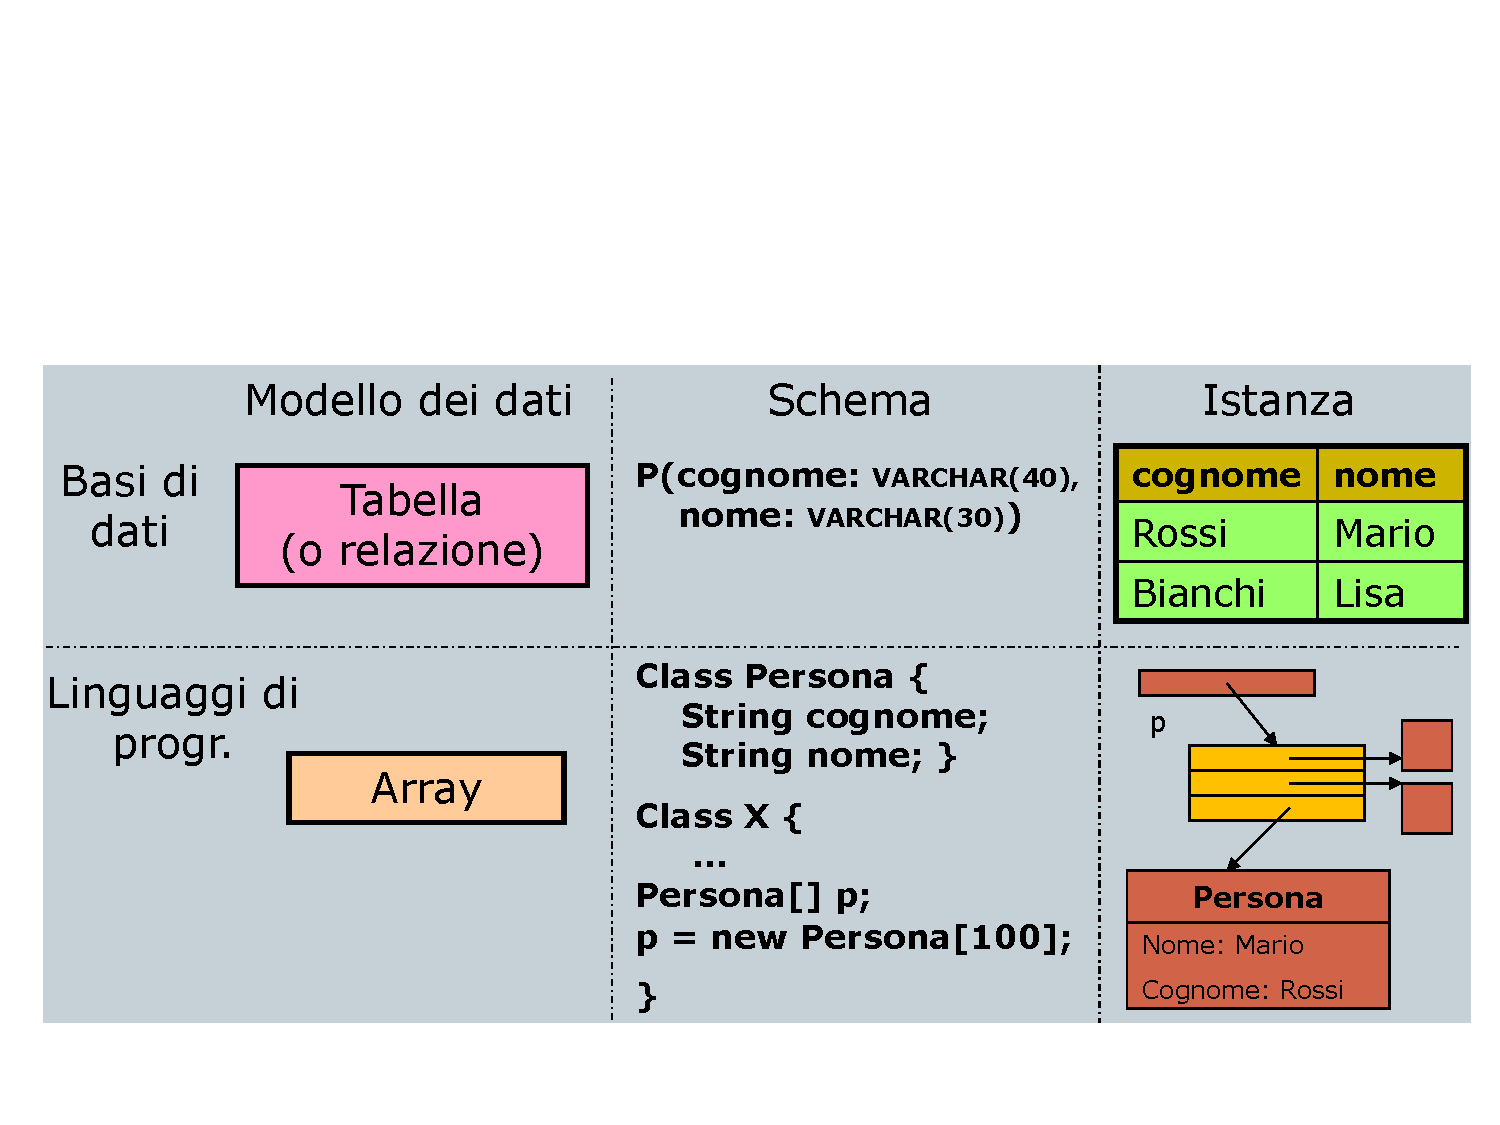
\includegraphics[width=0.9\textwidth]{img/diff_modello-schemi-istanze.pdf}
		\caption{Esempio di modello di dati, schema e istanza.}
	\end{figure}

	\newpage
	
	
	
	
	\subsection{Astrazione (architettura) dei DBMS}\label{Astrazione (architettura) dei DBMS}
	
	Esiste un'architettura standardizzata per i DMBS, la quale si caratterizza su tre livelli: \textbf{esterno}, \textbf{logico} e \textbf{interno}:
	
	\begin{itemize}
		\item[\ding{80}] \textbf{\emph{Schema logico.}} È la rappresentazione della \textbf{struttura} e delle \textbf{proprietà} della \textbf{base di dati} definita \underline{attraverso i costrutti} del modello dei dati del DBMS. In altre parole, descrive l'intera base di dati per mezzo del modello logico adottato dal DBMS (quindi relazione o ad oggetti).
		
		\item[\ding{72}] \textbf{\emph{Schema interno.}} È la rappresentazione della base di dati per mezzo delle \textbf{strutture fisiche di memorizzazione} (e.g. file sequenziale, file hash, ecc.).
		
		\item[\ding{73}] \textbf{\emph{Schema esterno.}}\label{schema esterno} Descrive una \textbf{porzione dello schema logico} di interesse per uno \textbf{specifico} utente o applicazione. \underline{Possono esistere più schemi} esterni che consentono di avere \underline{punti di vista differenti} senza cambiare la logica di base.
	\end{itemize}

	\begin{figure}[!htp]
		\centering
		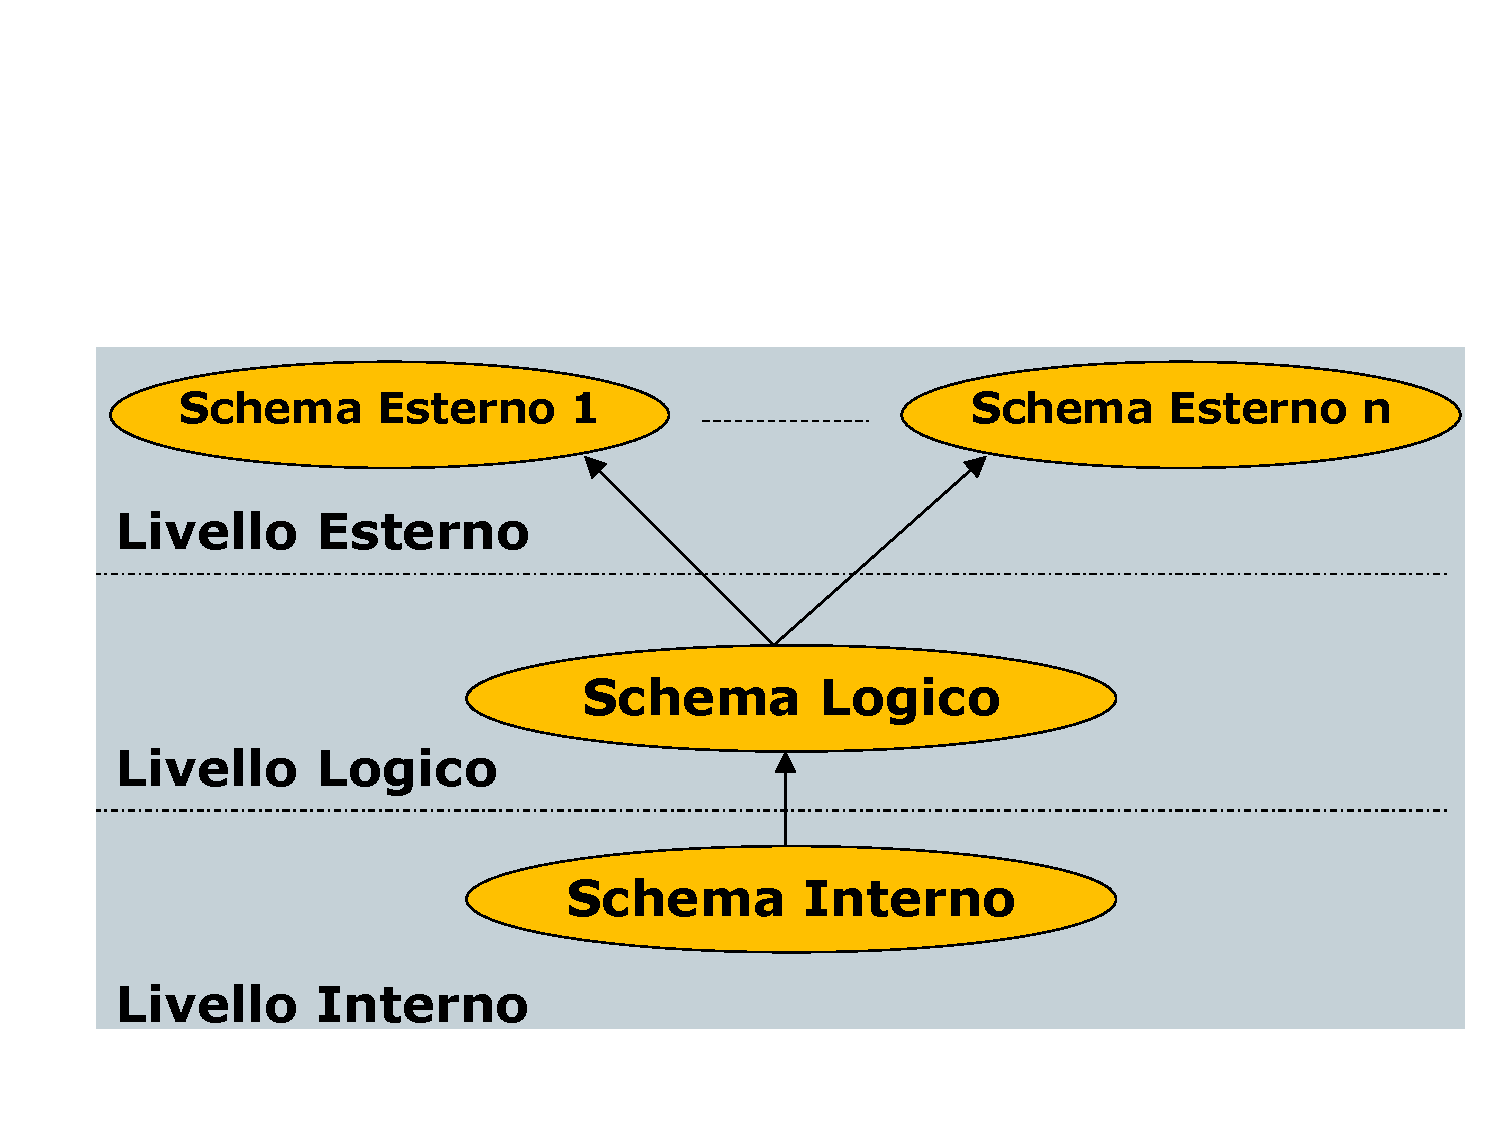
\includegraphics[width=0.8\textwidth]{img/arch_DBMS.pdf}
		\caption{Architettura generale di un DBMS.}
	\end{figure}

	\newpage
	
	
	
	
	\subsection{Indipendenza dei dati}
	
	L'architettura a livelli definita nel paragrafo \ref{Astrazione (architettura) dei DBMS} garantisce l' \textcolor{Red3}{\textbf{indipendenza dei dati}}, la \textbf{proprietà più importante} dei DBMS. L'\textbf{obbiettivo} è quello di poter fornire all'utente una basi di dati in grado di interagire con un \underline{elevato livello di astrazione}. Esistono due tipi di indipendenza:
	
	\begin{itemize}
		\item[\ding{42}] \textbf{\emph{Indipendenza \underline{fisica}.}} Lo schema logico della basi di dati è \underline{completamente} indipendente dallo schema interno. Quindi, l'interazione con il DBMS può essere effettuato in modo indipendente dalla struttura fisica dei dati.\newline
		\textcolor{Green4}{\textbf{Vantaggio:}} le modifiche \textbf{\underline{non}} influiscono sullo schema logico, cioè sulle applicazioni che lo utilizzano.
		
		\item[\ding{42}] \textbf{\emph{Indipendenza \underline{logica}.}} Gli \underline{schemi esterni} (definizione nel paragrafo:~\ref{schema esterno}) della base di dati sono \textbf{\underline{indipendenti}} dallo \underline{schema logico}. Quindi, è possibile interagire con il livello esterno in modo indipendente dal livello logico.\newline
		\textcolor{Green4}{\textbf{Vantaggio:}}
		\begin{enumerate}[label=\Roman*]
			\item \textbf{Aggiunta/Modifica} di uno schema \underline{esterno} in base alle esigenze di un nuovo utente, senza modificare lo schema logico;
			
			\item \textbf{Modifica} di uno schema logico mantenendo inalterate le strutture esterne.
		\end{enumerate}
	\end{itemize}

	\newpage
	
	


	\section{Metodologie e modelli per il progetto}
	
	\subsection{Ciclo di vita dei sistemi informativi}
	
	La progettazione di una base di dati costituisce solo una delle componenti del processo di sviluppo di un sistema informativo complesso e va quindi inquadrata in un contesto più ampio quello del \textbf{ciclo di vita} dei sistemi informativi:
	
	\begin{itemize}
		\item[\ding{42}] \textbf{\emph{Studio di fattibilità.}} Definisce i \underline{costi} delle varie alternative possibili e stabilisce le \underline{priorità di realizzazione} delle varie componenti del sistema.
		
		\item[\ding{42}] \textbf{\emph{Raccolta e analisi dei requisiti.}} Individua le proprietà e le funzionalità che il sistema informativo deve avere producendo una descrizione completa, ma generalmente informale.
		
		\item[\ding{42}] \textbf{\emph{Progettazione.}} Si divide in due fasi:
		\begin{itemize}
			\item \textbf{Progettazione dei dati.} Individua la struttura e l'organizzazione che i dati devono avere.
			
			\item \textbf{Progettazione delle applicazioni.} Definizione delle caratteristiche dei programmi applicativi.
		\end{itemize}
		
		\item[\ding{42}] \textbf{\emph{Implementazione (su un DBMS).}} È la realizzazione del sistema informativo secondo la struttura e le caratteristiche fornite durante la fase di progettazione. In questa fase \underline{viene costruita e popola la base di dati}.
		
		\item[\ding{42}] \textbf{\emph{Validazione e collaudo.}} Verifica il corretto funzionamento e la qualità del sistema informativo.
		
		\item[\ding{42}] \textbf{\emph{Funzionamento.}} Il sistema informativo diventa operativo ed esegue i compiti per i quali è stato progettato.
	\end{itemize}

	\noindent
	Spesso il processo \textbf{non} è strettamente sequenziale. Infatti, come si vede dalla seguente figura, durante l'esecuzione di una delle attività sopraelencate, è necessario rivedere decisioni prese nell'attività precedente.
	
	\begin{figure}[!htp]
		\centering
		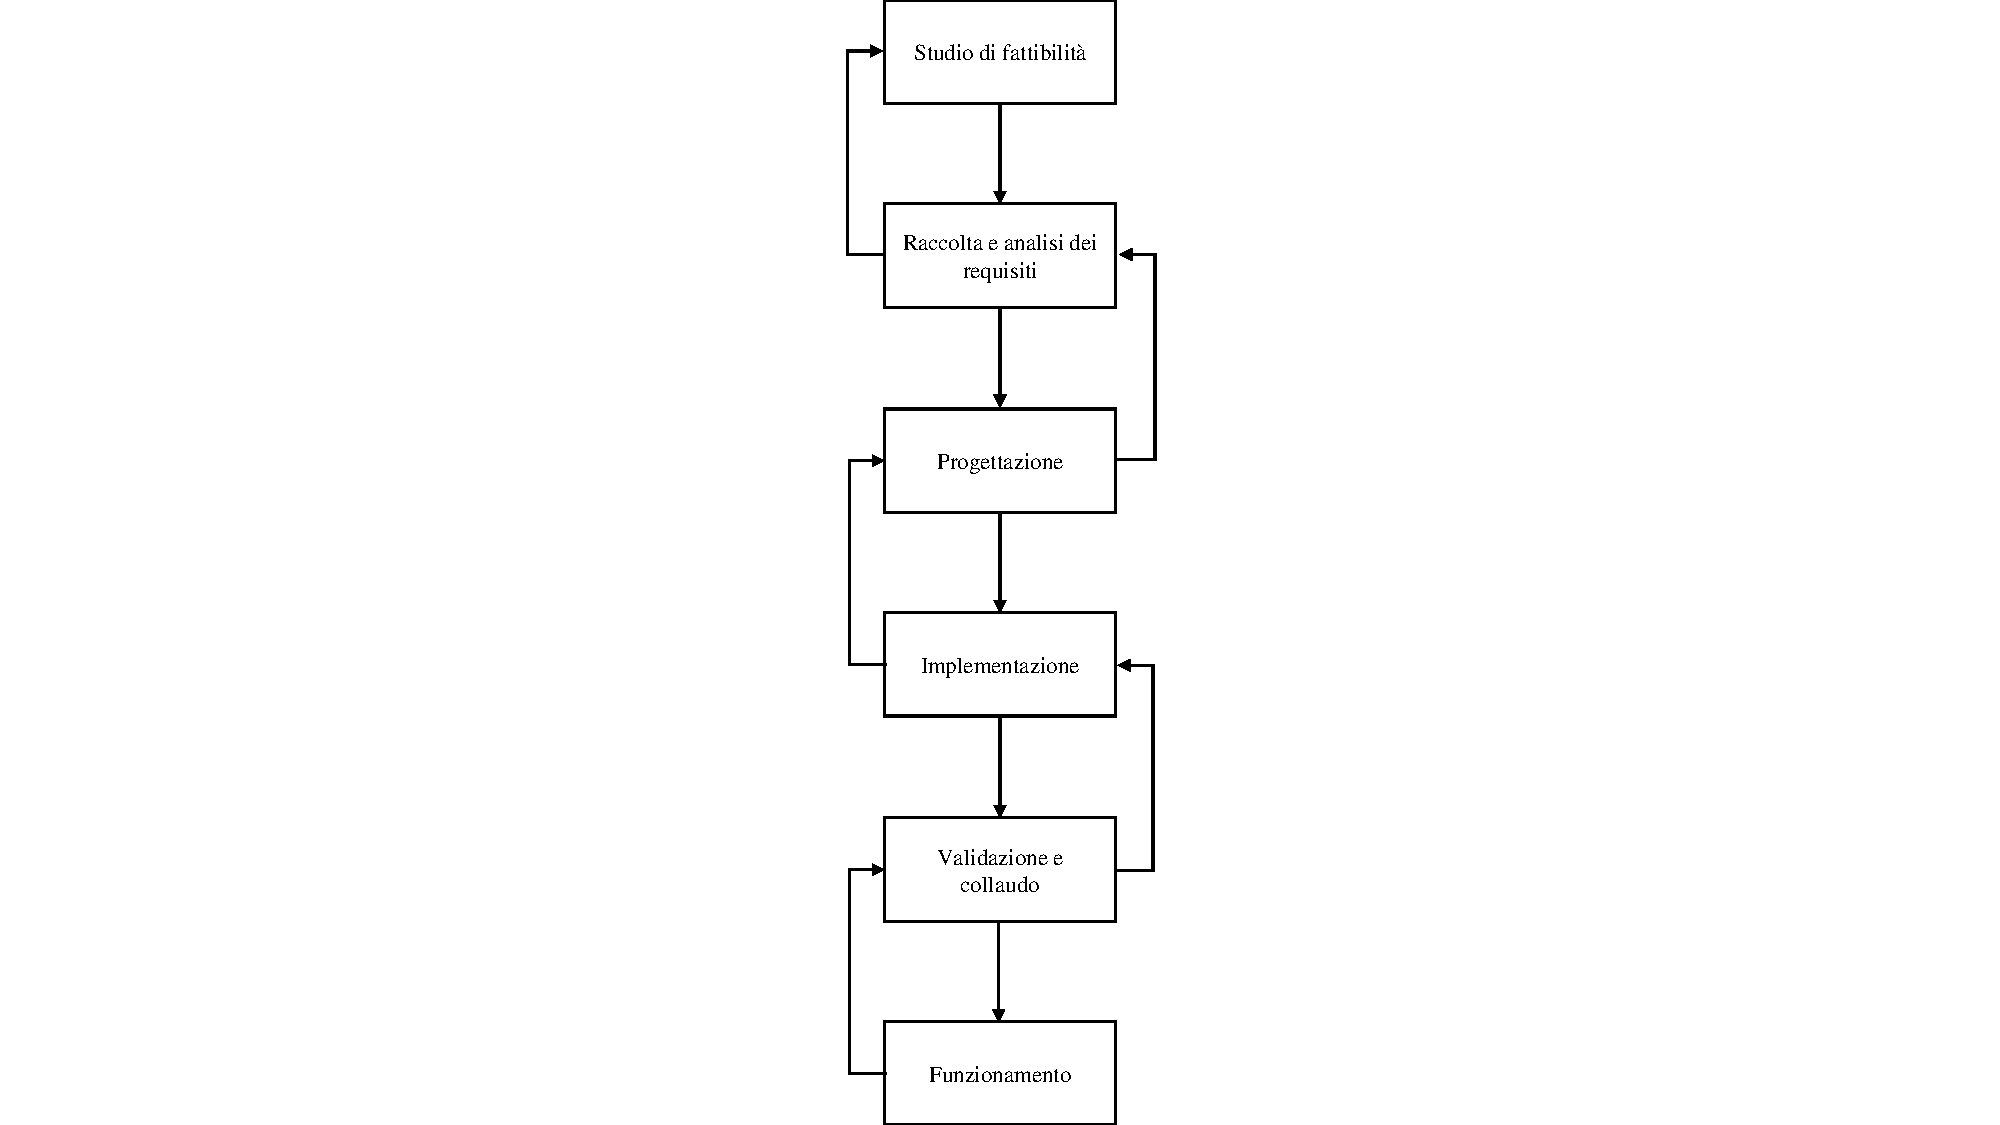
\includegraphics[width=0.4\textwidth]{img/ciclo_di_vita_sis_inf.pdf}
		\caption{Ciclo di vita di un sistema informativo.}
	\end{figure}

	\newpage
	
	
	
	
	\subsection{Metodologie di progettazione e basi di dati}
	
	Una \textbf{metodologia di progettazione} consiste in:
	
	\begin{itemize}
		\item[\ding{51}] \textbf{Decomposizione} dell'intera attività di progetto in passi successivi indipendenti tra loro.
		
		\item[\ding{51}] \textbf{Strategie} da seguire nei vari passi e \textbf{criteri} nel caso di alternative.
		
		\item[\ding{51}] \textbf{Modelli di riferimento} per descrivere i dati in ingresso e uscita delle varie fasi.
	\end{itemize}

	\noindent
	Le \textbf{proprietà} che una metodologia deve garantire sono:
	
	\begin{itemize}
		\item[\ding{72}] \textbf{\emph{Generalità}} rispetto alle applicazioni e ai sistemi in gioco;
		
		\item[\ding{72}] \textbf{\emph{Qualità del prodotto}} in termini di correttezza, completezza ed efficienza rispetto alle risorse impiegate;
		
		\item[\ding{72}] \textbf{\emph{Facilità d'uso}} delle strategie e dei modelli di riferimento.
	\end{itemize}

	%\newpage

	Negli anni si è \emph{consolidata una metodologia} di progetto che ha dato prova di soddisfare pienamente le proprietà descritte. Si basa sull'idea di separare le decisioni relative a \dquotes{cosa} rappresentare in una base di dati (prima fase), da quelle relative a \dquotes{come} farlo (seconda e terza fase):
	
	\begin{itemize}
		\item[\ding{42}] \textbf{Progettazione concettuale.}\newline
		\textcolor{Red3}{\textbf{Obbiettivo:}} rappresentare le specifiche informali della realtà di interesse in termini di una descrizione formale e completa. La \textbf{\underline{rappresentazione}} \textbf{\underline{deve essere indipendente}} dai criteri di rappresentazione utilizzati nei sistemi di gestione di basi di dati.\newline
		\textcolor{Green4}{\textbf{Prodotto di questa fase:}} \underline{schema concettuale}. È un documento formale che rappresenta il contenuto della base di dati in modo indipendente dall'implementazione (DBMS).\newline
		\textcolor{Blue3}{\textbf{Applicazione:}} cercare di rappresentare il \textbf{contenuto informativo} della base di dati, senza preoccuparsi né della modalità con le quali queste informazioni verranno codificate in un sistema reale, né dell'efficienza dei programmi che faranno uso di queste informazioni.\label{progettazione concettuale}
		
		\item[\ding{42}] \textbf{Progettazione logica.}\newline
		\textcolor{Red3}{\textbf{Obbiettivo:}} traduzione dello schema concettuale prodotto nella fase precedente, in termini del modello di rappresentazione dei dati adottato dal sistema di gestione di base di dati a disposizione.\newline
		\textcolor{Green4}{\textbf{Prodotto di questa fase:}} \underline{schema logico}.\newline
		\textcolor{Blue3}{\textbf{Applicazione:}} durante la traduzione, le scelte progettuali si \underline{devono} basare anche su criteri di ottimizzazione delle operazioni da effettuare sui dati.\label{progettazione logica}
		
		\item[\ding{42}] \textbf{Progettazione fisica.}\newline
		\textcolor{Red3}{\textbf{Obbiettivo:}} lo schema logico viene completato con la specifica dei parametri fisici di memorizzazione dei dati.\newline
		\textcolor{Green4}{\textbf{Prodotto di questa fase:}} \underline{schema fisico}.\newline\label{progettazione fisica}
	\end{itemize}

	\newpage
	
	
	
	
	\subsection{Il modello Entità-Relazione (E-R)}
	
	Il \textcolor{Red3}{\textbf{\emph{modello Entità-Relazione}}} è un modello \textbf{concettuale} di dati, quindi utilizzato nella \textbf{progettazione concettuale}, e fornisce una serie di strutture, chiamati \textbf{\emph{costrutti}}, atte a descrivere la realtà di interesse in una maniera facile da comprendere e che prescinde dai criteri di organizzazione dei dati nei calcolatori.
	
	I \underline{costrutti vengono utilizzati} per \textbf{definire schemi} che \textbf{descrivono l'organizzazione e la struttura delle occorrenze} (o \textbf{istanze}) \textbf{dei dati}, ovvero, dei valori assunti dai dati al variare del tempo.
	
	\noindent
	Si possono \underline{riassumere le caratteristiche} del modello Entità-Relazione:
	
	\begin{itemize}
		\item[\ding{42}] \textcolor{SpringGreen4}{\textbf{\emph{Modello concettuale}.}} Utilizzato durante la progettazione concettuale (definizione al paragrafo~\ref{progettazione concettuale}) di una base di dati.
		
		\item[\ding{42}] \textcolor{SpringGreen4}{\textbf{\emph{Strumenti formali}.}} Vengono messi a disposizione diversi strumenti per definire la \textbf{struttura} e le \textbf{proprietà} di una base di dati (\emph{esempio i costrutti}).
		
		\item[\ding{42}] \textcolor{SpringGreen4}{\textbf{\emph{Indipendente dalla tecnologia}.}} Essendo un modello astratto, l'obbiettivo è quello di definire la struttura e le proprietà della base di dati (\underline{non di implementarla!}).
		
		\item[\ding{42}] \textcolor{SpringGreen4}{\textbf{\emph{Formale}.}} È facile da utilizzare nonostante non ammetta ambiguità.
		
		\item[\ding{42}] \textcolor{SpringGreen4}{\textbf{\emph{Grafico}.}} La sintassi è prettamente grafica e questo aumenta anche la leggibilità.
	\end{itemize}

	\newpage
	
	
	
	
	\subsection{I costrutti principali del modello}
	
	Si analizzano i principali costrutti di questo modello: entità (pagina~\pageref{entità}), relazioni(pagina~\pageref{relazioni}) e attributi (pagina~\pageref{attributi}).
	
	\subsubsection{Entità}\label{entità}
	\textcolor{Red3}{\textbf{Definizione.}} Rappresentano \textbf{classi di oggetti} (per esempio, fatti, cose, persone) \textbf{che hanno proprietà comuni ed esistenza \dquotes{autonoma} ai fini dell'applicazione di interesse}. Per esempio, \dquotes{città, dipartimento, impiegato, acquisto e vendita} sono entità di un'applicazione aziendale. Inoltre, \textbf{ogni entità ha un nome identificativo}, il quale deve essere \textbf{univoco}. In sintesi:
	
	\begin{itemize}
		\item Hanno \textbf{proprietà comuni};
		\item Hanno \textbf{esistenza autonoma};
		\item Hanno \textbf{identificazione univoca}.
	\end{itemize}

	\noindent
	\textcolor{Green4}{\textbf{Sintassi grafica.}}
	
	\begin{figure}[!htp]
		\centering
		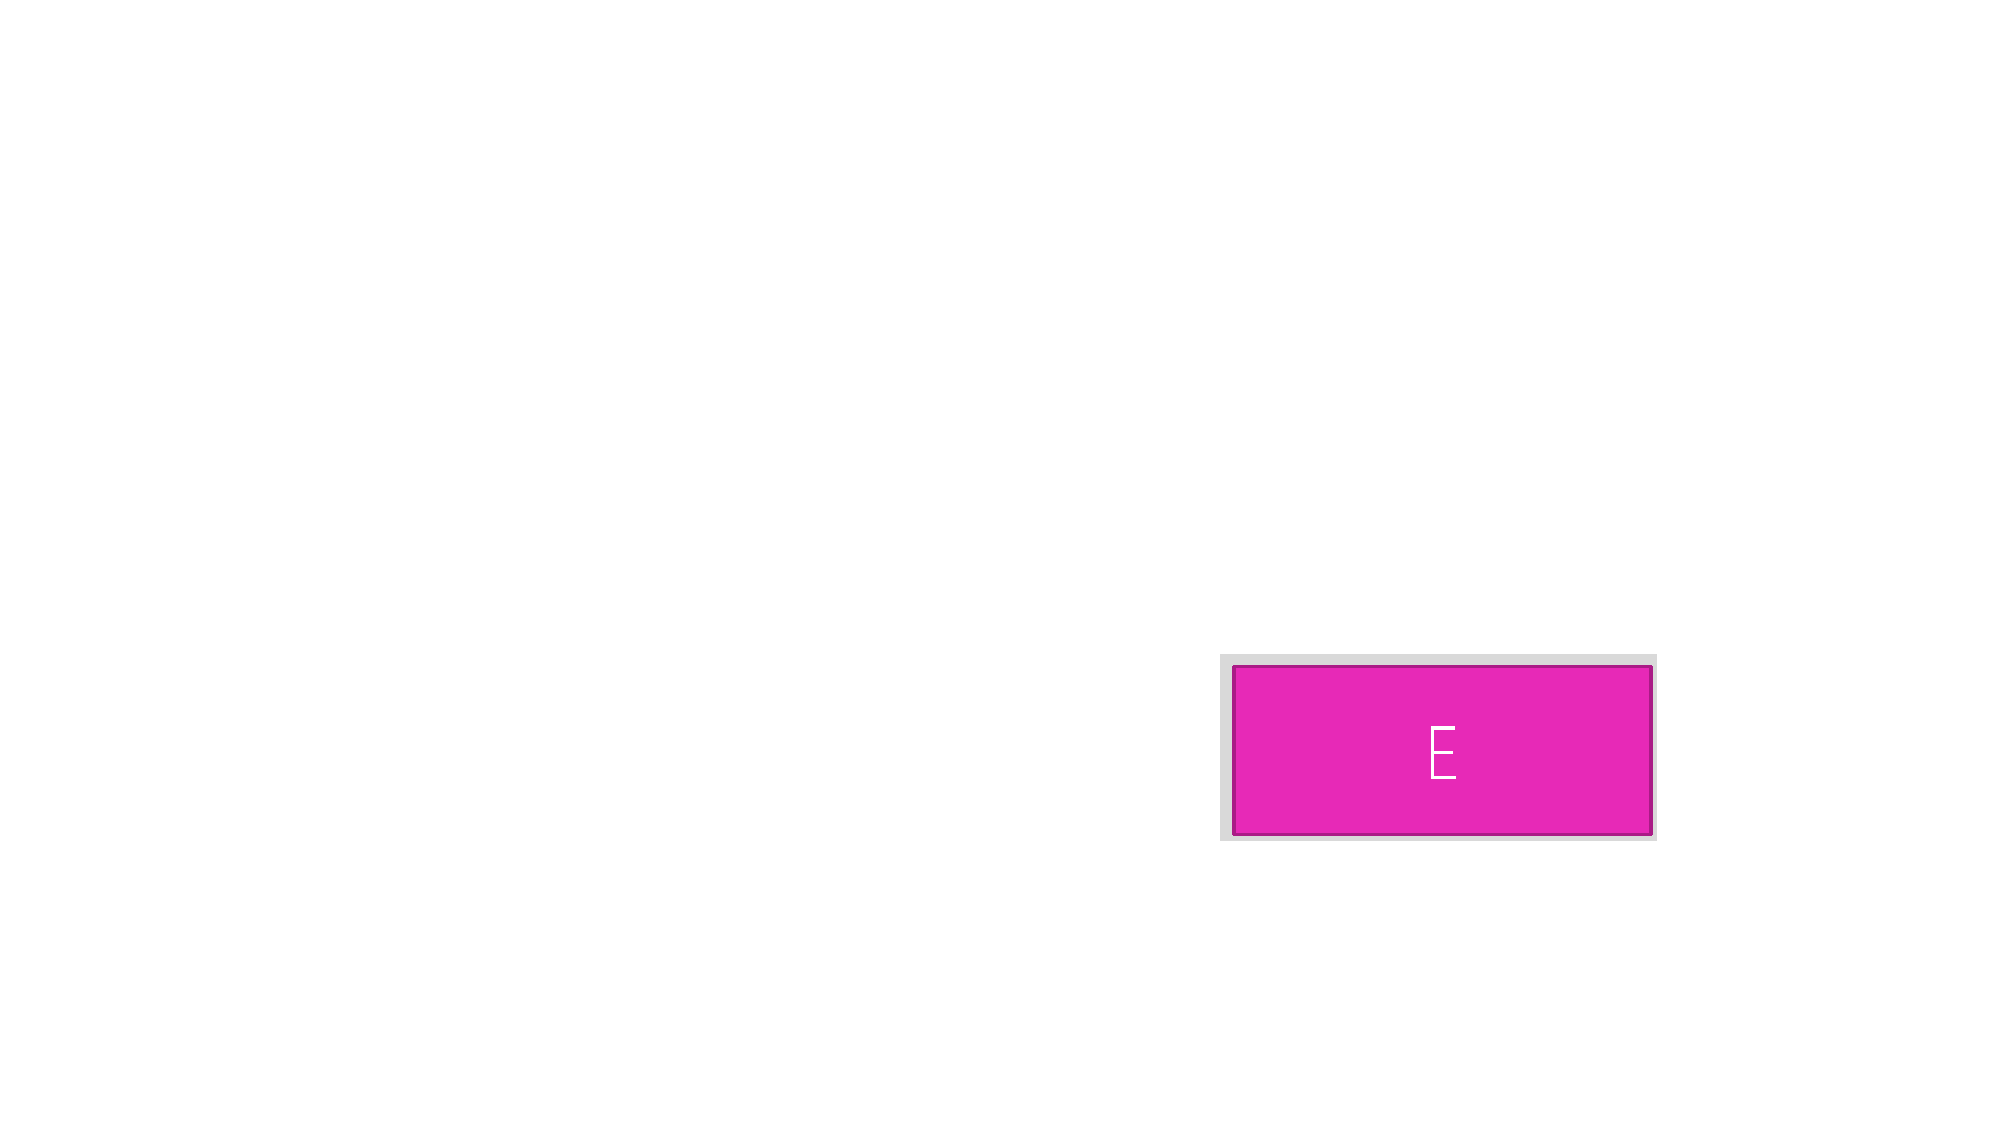
\includegraphics[width=0.5\textwidth]{img/entita_def.pdf}
		\caption{Sintassi grafica dell'entità.}
	\end{figure}

	\noindent
	\textcolor{blue}{\textbf{Istanza (o occorrenza).}} Un'\textbf{istanza} (o occorrenza) di un'entità è un \textbf{oggetto della classe che l'entità rappresenta}. Le città di Roma, Milano e Palermo sono esempi di occorrenze dell'entità \dquotes{Città}.\newline
	\textbf{\underline{Attenzione!}} L'istanza di un'entità \textbf{\emph{non è un valore}} che identifica un oggetto (per esempio, il cognome dell'impiegato o il suo codice fiscale),\textbf{\emph{ ma è l'oggetto stesso}} (l'impiegato in \dquotes{carne e ossa}). Quindi, un'\textbf{istanza ha un'esistenza indipendente dalle proprietà a esso associate}.
	
	Un’istanza dell’entità $E$ è un oggetto appartenente alla classe rappresentata da $E$. Si indica con $I(E)$ l’insieme delle istanze di $E$ che esistono nella base di dati in un certo istante.
	
	\newpage
	
	
	
	
	\subsubsection{Relazioni (o associazioni)}\label{relazioni}
	
	\textcolor{Red3}{\textbf{Definizione.}} Rappresentano \textbf{legami logici}, significativi per l'applicazione di interesse, \textbf{tra due o più entità}. Per esempio, \dquotes{Residenza} è una relazione che sussiste tra le entità \dquotes{Città} e \dquotes{Impiegato}.Nello schema E-R, \textbf{ogni relazione ha un nome identificativo univoco}.
	
	\noindent
	Le relazioni possono essere di \textbf{tipo}:
	
	\begin{itemize}
		\item \textbf{\emph{Ricorsive}}, ovvero \textbf{relazioni tra un'entità e se stessa}. Per esempio, la relazione \dquotes{Collega} sull'entità \dquotes{Impiegato} connette coppie di impiegati che lavorano insieme.
		
		\item \textbf{\emph{n-arie}}, ovvero \textbf{relazioni che coinvolgono più di due entità}. Per esempio, la relazione \dquotes{Fornitura} tre le tre entità \dquotes{Fornitore, Prodotto e Dipartimento} descrive il fatto che un fornitore rifornisce un dipartimento di un certo prodotto.
	\end{itemize}

	\noindent
	\textbf{\underline{Nota fondamentale:}} \textbf{per eseguire una relazione, le entità devono essere tutte piene o con almeno un dato all'interno.} \newline
	
	\noindent
	\textcolor{Green4}{\textbf{Sintassi grafica.}} Una relazione $R$ si rappresenta nello schema con un \textbf{rombo} a cui si collegano attraverso linee spezzate le entità coinvolte nella relazione. Il nome della relazione viene scritto a fianco del rombo.
	
	\begin{figure}[!htp]
		\centering
		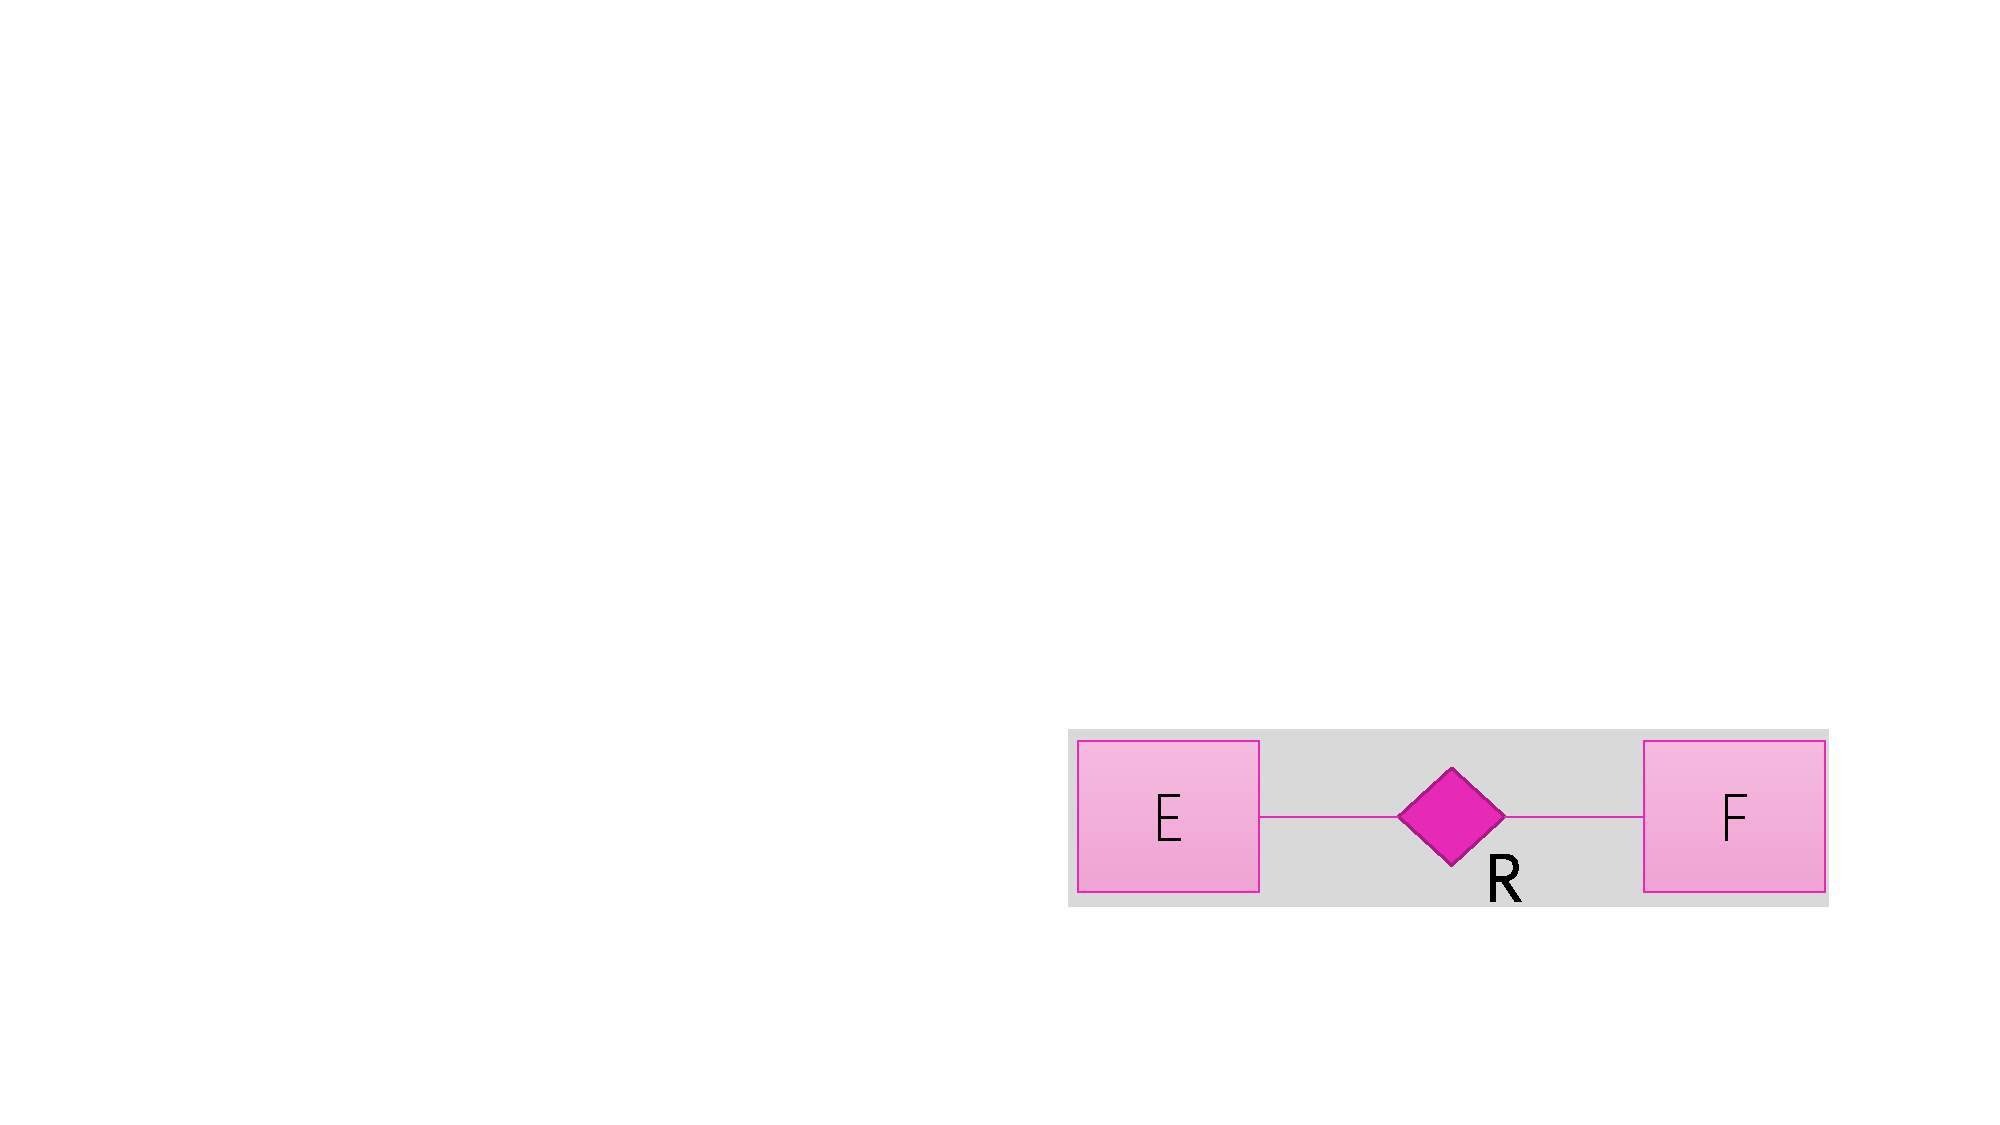
\includegraphics[width=0.6\textwidth]{img/relazione_def.pdf}
		\caption{Sintassi grafica della relazione.}
	\end{figure}

	\noindent
	\textcolor{blue}{\textbf{Istanza (o occorrenza).}} Un'istanza di relazione è un'\textbf{ennupla costituita da istanze di entità, una per ciascuna delle entità coinvolte}.
	
	\noindent
	Data una relazione $R$ tra $n$ entità $E_1, \cdots, E_n$, un’istanza della relazione $R$ è una ennupla di istanze di entità:
	
	\begin{equation*}
		\left(e_1, \cdots, e_n\right) \text{ dove } e_i \in I(E_i), 1\le i \le n
	\end{equation*}

	\noindent
	Infine, esiste una relazione importante. Data una relazione $R$ tra $n$ entità, vale sempre la seguente proprietà sull’insieme delle istanze di $R (I(R))$:
	
	\begin{equation*}
		I(R) \subseteq I(E_1) \times \cdots \times I(E_n)
	\end{equation*}
	
	\newpage
	
	
	
	
	\subsubsection{Attributi}\label{attributi}
	
	\textcolor{Red3}{\textbf{Definizione.}} Descrivono le \textbf{proprietà elementari} di entità o relazioni che sono di interesse ai fini dell'applicazione. Per esempio, \dquotes{Cognome, Stipendio ed Età} sono possibili attributi dell'entità \dquotes{Impiegato}.
	
	Un attributo associa a ciascun istanza di entità (o relazione) \textbf{\underline{uno e un solo}} valore appartenente a un insieme, chiamato \textbf{\emph{dominio}}, che contiene i valori ammissibili per l'attributo. Per esempio, l'attributo \dquotes{Cognome} dell'entità \dquotes{Impiegato} può avere come dominio l'insieme delle stringhe di $20$ caratteri.
	
	L'attributo può essere visto come una \textbf{funzione che ha come dominio le istanze dell'entità} (o relazione) e come \textbf{codominio l'insieme dei valori ammissibili}:
	
	\begin{equation*}
		f_{a} : I\left(E\right) \rightarrow D
	\end{equation*}

	\begin{itemize}
		\item $a$ è un attributo dell'entità $E$;
		
		\item $I\left(E\right)$ è l'insieme delle istanze di $E$;
		
		\item $D$ è l'insieme dei valori ammissibili.
	\end{itemize}
	
	\noindent
	\textcolor{Green4}{\textbf{Sintassi grafica.}}
	
	\begin{figure}[!htp]
		\centering
		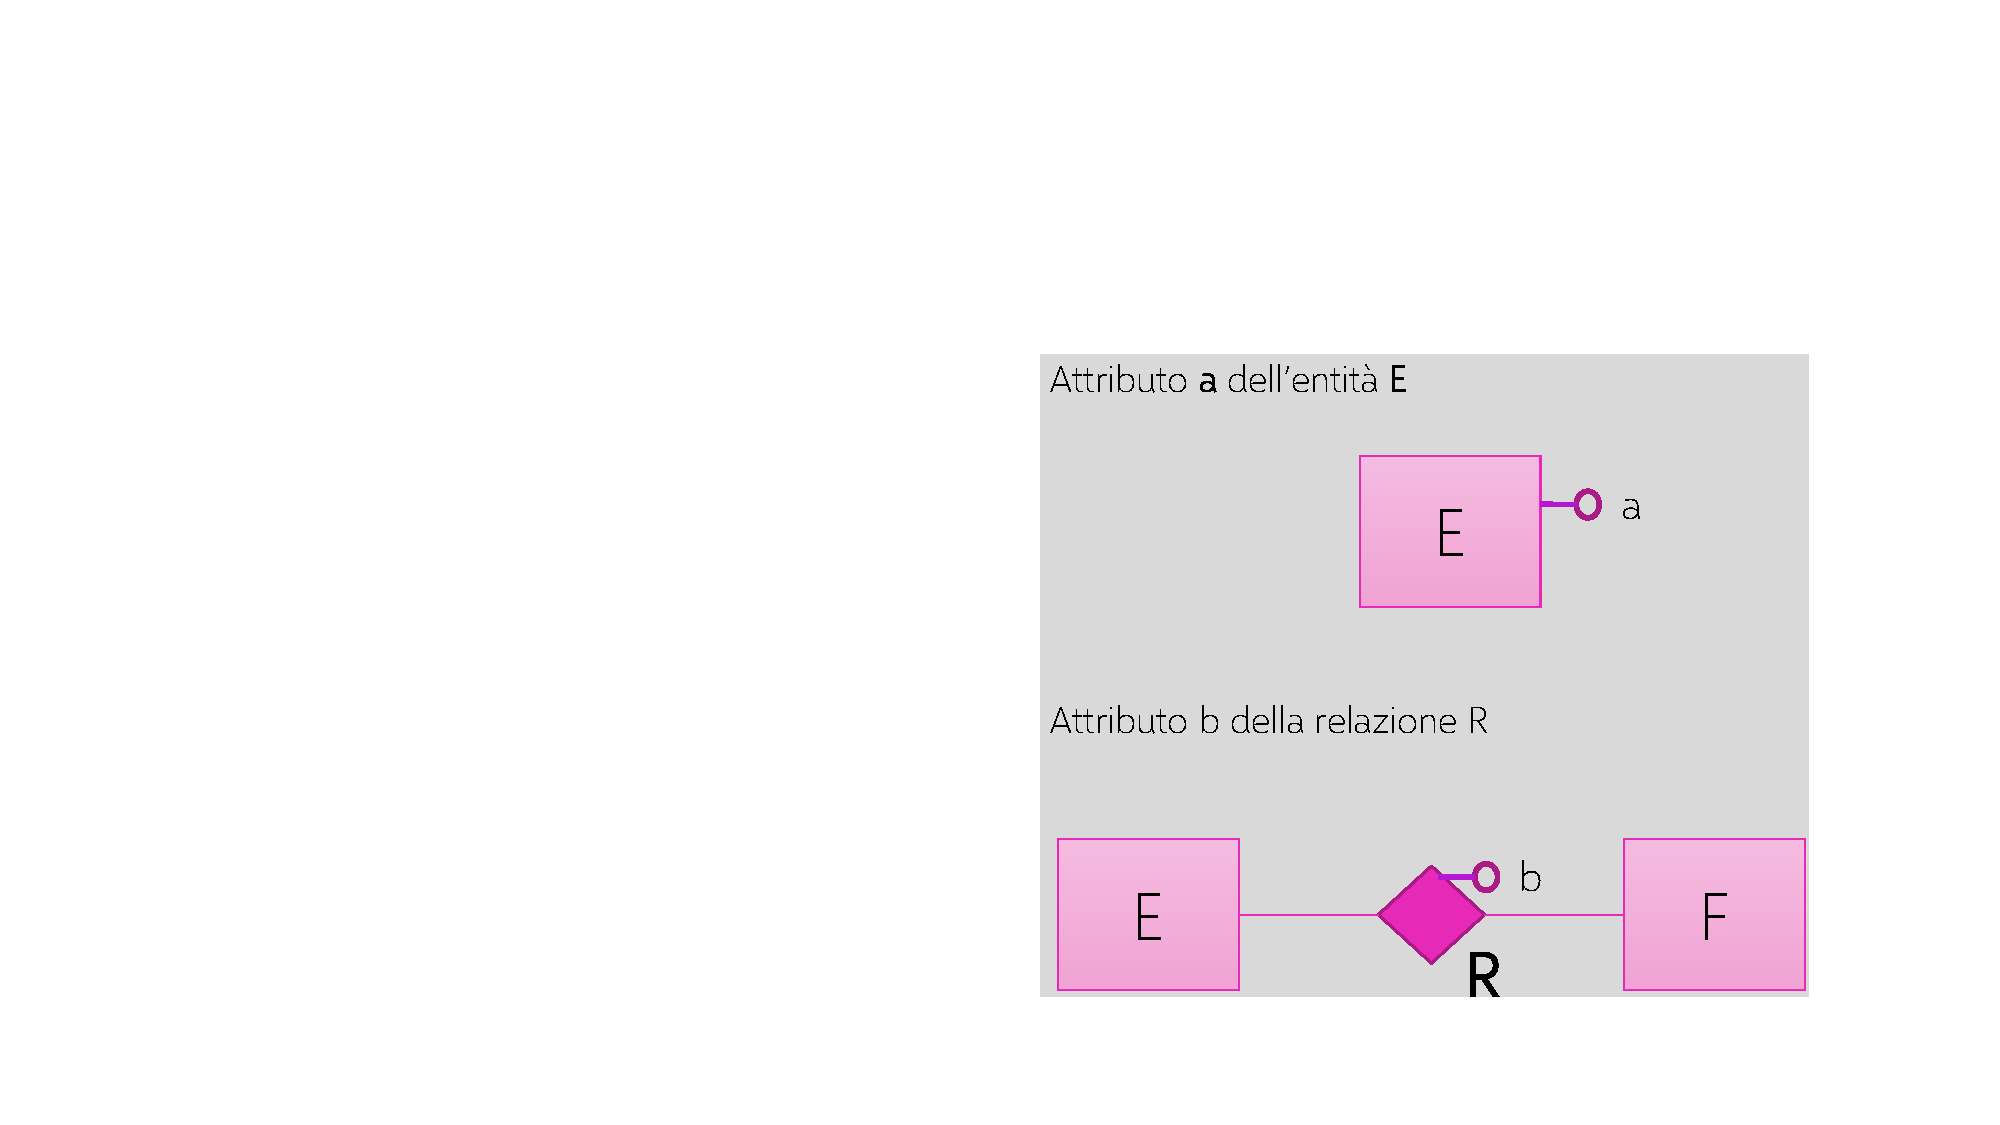
\includegraphics[width=0.5\textwidth]{img/attributo_def.pdf}
		\caption{Sintassi grafica dell'attributo.}
	\end{figure}
	
	\noindent
	\textcolor{blue}{\textbf{Istanza (o occorrenza).}} Dato un attributo $a$ di un'entità $E$ (o relazione $R$), un'istanza di $a$ è il valore $v$ che esso assume su un'istanza di $E$ (o istanza di $R$).
	
	Quindi, data un'istanza $e$ dell'entità $E$ (o relazione $R$), l'istanza di un suo attributo $a$ si ottiene dalla funzione $f_{a}$ applicata a $e$:
	
	\begin{equation*}
		\text{valore di } a \text{ su } e = f_{a}\left(e\right)
	\end{equation*}

	\noindent
	\fbox{%
		\parbox{\textwidth}{%
			\textcolor{Red3}{\textbf{\underline{Attributi composti.}}}\newline
			
			Questo tipo di attributo viene introdotto solo a fini didattici, ma l'obbiettivo è quello di usare unicamente gli attributi normali. Talvolta potrebbe tornare comodo raggruppare \textbf{attributi di una medesima entità o relazione che presentano affinità nel loro significato o uso}: tale insieme prende il nome di \textbf{attributo composto}. Per esempio, gli attributi \dquotes{Via, Numero civico e CAP} dell'entità \dquotes{Persona} per formare l'attributo composto \dquotes{Indirizzo}.
		}%
	}

	\newpage
	
	\subsection{Altri costrutti del modello}
	
	I rimanenti costrutti del modello E-R sono le cardinalità delle relazioni e degli attributi e gli identificatori.
	
	\subsubsection{Cardinalità delle relazioni}
	
	\textcolor{Red3}{\textbf{Definizione.}} Le \textbf{cardinalità} vengono \textbf{specificate per ciascuna entità collegata ad una relazione} e descrivono il \textbf{numero minimo e massimo di occorrenze} di relazione a cui una occorrenza dell'entità può partecipare.
	
	Più formalmente, data una relazione $R$ i vincoli di cardinalità vengono specificati per ogni entità $E_{i}$ coinvolta nella relazione $R$ e specificano: il numero massimo e il numero minimo di istanze di $R$ a cui un'istanza di $E_{i}$ deve/può partecipare.
	
	In parole povere, dicono quante volte, in una relazione tra entità, un'istanza di una di queste entità può essere legata a istanze delle altre entità coinvolte. \textbf{\underline{Per esempio}}, in una relazione \dquotes{Assegnamento} tra le entità \dquotes{Impiegato} e \dquotes{Incarico} si specifica per la prima entità una cardinalità minima pari a uno e una cardinalità massima pari a cinque. Quindi, un impiegato può partecipare a un minimo di una occorrenza e a un massimo di cinque occorrenze della relazione \dquotes{Assegnamento}.\newline
	
	\noindent
	\textbf{\underline{N.B.}} Specificando \textbf{zero come cardinalità minima}, si impone che un'occorrenza può apparire oppure no.\newline
	
	\noindent
	È possibile \textbf{assegnare un qualunque valore intero \underline{non negativo} a una cardinalità di una relazione con l'\underline{unico vincolo} che la cardinalità \emph{minima} deve essere \underline{minore o uguale} della cardinalità \emph{massima}}.
	
	\noindent
	Tuttavia, nella maggior parte dei casi, è sufficiente utilizzare solamente tre simboli: $0$, $1$ e $N$ (molti).
	
	\begin{itemize}[label=\ding{72}]
		\item \textbf{\underline{Cardinalità minima.}}
		\begin{itemize}
			\item \textbf{Zero.} La partecipazione dell'entità relativa è \emph{\textbf{opzionale}};
			\item \textbf{Uno.} La partecipazione dell'entità relativa è \emph{\textbf{obbligatoria}}.
		\end{itemize}
	
		\item \textbf{\underline{Cardinalità massima.}}
		\begin{itemize}
			\item \textbf{Uno.} La partecipazione dell'entità relativa è come una funzione che associa a una occorrenza dell'entità una sola occorrenza (o nessuna) dell'altra entità che partecipa alla relazione;
			\item \textbf{N (molti).} Esiste un'associazione con un numero arbitrario di occorrenze dell'altra entità.
		\end{itemize}
	\end{itemize}

	\noindent
	\textcolor{Green4}{\textbf{Sintassi grafica.}}
	
	\begin{figure}[!htp]
		\centering
		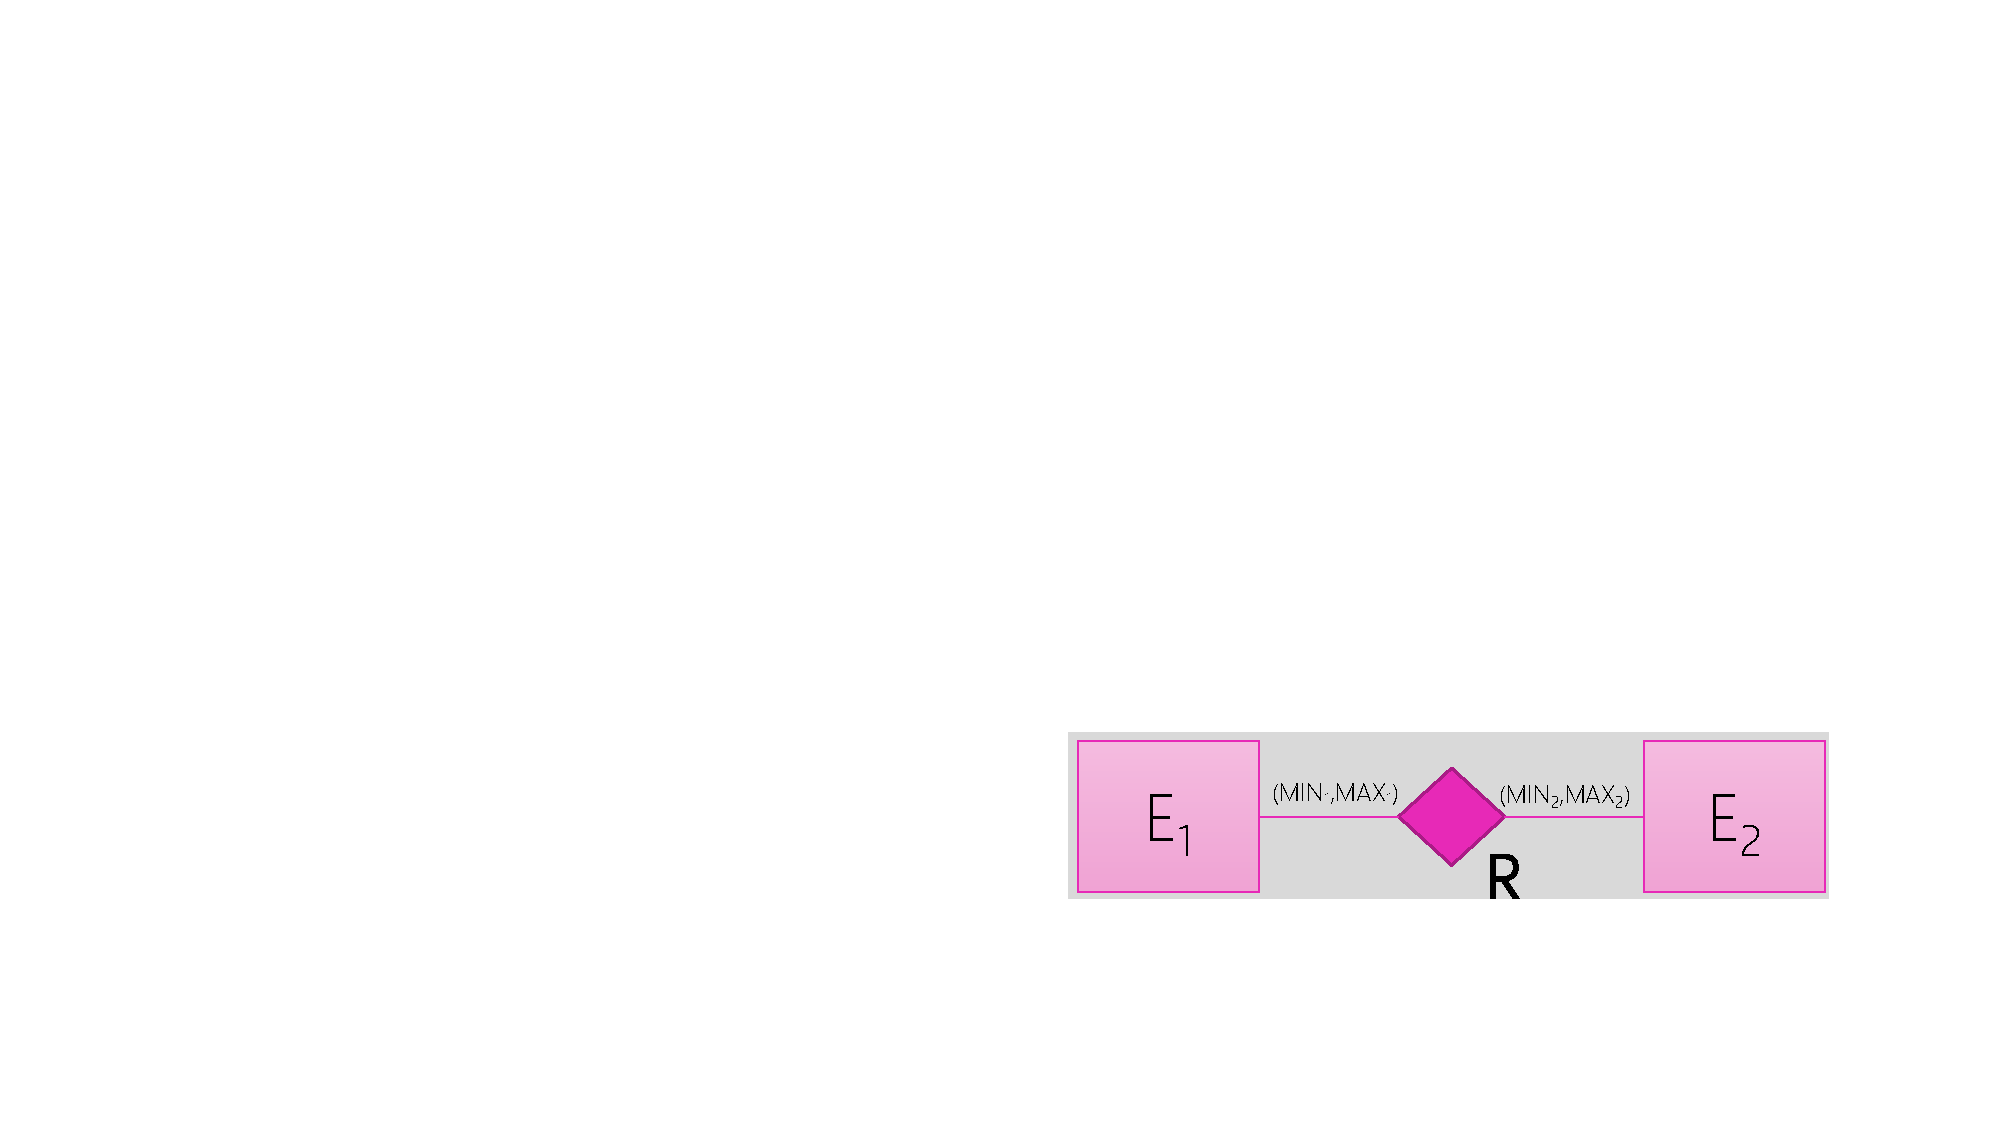
\includegraphics[width=0.52\textwidth]{img/cardinalita_def.pdf}
		\caption{Sintassi grafica della cardinalità.}
	\end{figure}
	
	\newpage

	\subsubsection{Cardinalità degli attributi}
	
	\textcolor{Red3}{\textbf{Definizione.}} Le \textbf{cardinalità degli attributi} è specificata per gli attributi di entità o relazione e hanno l'\textbf{\underline{obbiettivo}} di \textbf{descrivere il numero minimo e massimo di valori dell'attributo associati a ogni occorrenza di entità o relazione}.\newline
	
	\noindent
	Solitamente, il valore di cardinalità pari $\left(1,1\right)$,  ma si possono avere vari casi:
	
	\begin{itemize}
		\item $\left(1, 1\right) \longrightarrow$ L'attributo rappresenta una funzione che associa ad ogni occorrenza di entità un solo valore dell'attributo. Solitamente viene omesso e, come si vede nell'immagine~\ref{esempio cardinalità attributi}, la \dquotes{Persona} ha uno e un solo \dquotes{Cognome};
		
		\item $\left(0, 1\right) \longrightarrow$ L'attributo con cardinalità minima pari a zero vuol dire che è \textbf{opzionale} e la cardinalità massima pari a uno indica che nel \textbf{caso in cui esista}, questo valore è \textbf{unico}. Nell'esempio in figura~\ref{esempio cardinalità attributi}, la persona può avere solo un numero di patente, ma potrebbe anche non avercela;
		
		\item $\left(1, N\right) \longrightarrow$ L'attributo deve esistere, ma contiene più valori, quindi si dice che è \textbf{multivalore};
		
		\item $\left(0, N\right) \longrightarrow$ L'attributo è opzionale, ma se esiste può essere multivalore.
	\end{itemize}
	
	\begin{figure}[!htp]
		\centering
		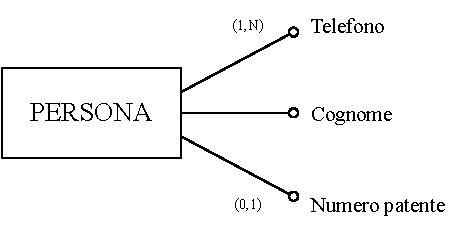
\includegraphics[width=0.5\textwidth]{img/cardinalita-attributi_def.pdf}
		\caption{Esempio di cardinalità degli attributi.}\label{esempio cardinalità attributi}
	\end{figure}

	\newpage

	\subsubsection{Identificatori}
	
	\textcolor{Red3}{\textbf{Definizione.}} Vengono \textbf{specificati per ciascuna entità} di uno schema e \textbf{descrivono i} concetti (\textbf{attributi e/o entità}) dello schema che \textbf{permettono di identificare in maniera \underline{univoca} le occorrenze delle entità}.\newline
	
	\noindent
	È assolutamente \textbf{vietato inserire uno o più identificatori all'interno di una relazione}. Quindi, quest'ultima non può avere identificatori interni!\newline
	
	\noindent
	\textbf{Per esempio}, un identificato interno per l'entità \dquotes{Automobile} con attributi \dquotes{Modello, Targa e Colore} è l'attributo \dquotes{Targa}, in quanto non possono esistere due automobili con la stessa targa e quindi due occorrenze dell'entità \dquotes{Automobile} con gli stessi valori sull'attributo \dquotes{Targa}.\newline
	
	\noindent
	Un'entità $E$ può essere identificata da altre entità solo se tali entità sono coinvolte in una relazione a cui $E$ partecipa con cardinalità $\left(1, 1\right)$. Nei casi in cui l'identificazione di un'entità è ottenuta utilizzando altre entità si parla di \textbf{identificatore \underline{esterno}}. \newline
	Per comprendere meglio si espone un \textbf{esempio}. Per identificare univocamente uno studente serve, oltre al numero di matricola, anche la relativa università. Quindi, un identificatore corretto per l'entità \dquotes{Studente} in questo schema è costituito dall'attributo \dquotes{Matricola} e dall'entità \dquotes{Università}.\newline
	
	\noindent
	Quindi, in generale:
	
	\begin{itemize}
		\item Un identificatore può \textbf{coinvolgere uno o più attributi}, ognuno dei quali deve avere cardinalità $\left(1,1\right)$;
		
		\item Un identificatore esterno può \textbf{coinvolgere una o più entità}, ognuna delle quali deve essere membro di una relazione alla quale l'entità da identificare partecipa con cardinalità $\left(1,1\right)$;
		
		\item Un identificatore esterno può \textbf{coinvolgere un'entità che è a sua volta identificata esternamente}, purché non vengano generati, in questa maniera, cicli di identificazione esterna;
		
		\item Ogni \textbf{entità deve avere almeno un identificatore} (interno o esterno), ma ne può avere in generale più di uno.
	\end{itemize}

	\newpage

	\noindent
	\textcolor{Green4}{\textbf{Sintassi grafica.}}
	
	\begin{figure}[!htp]
		\centering
		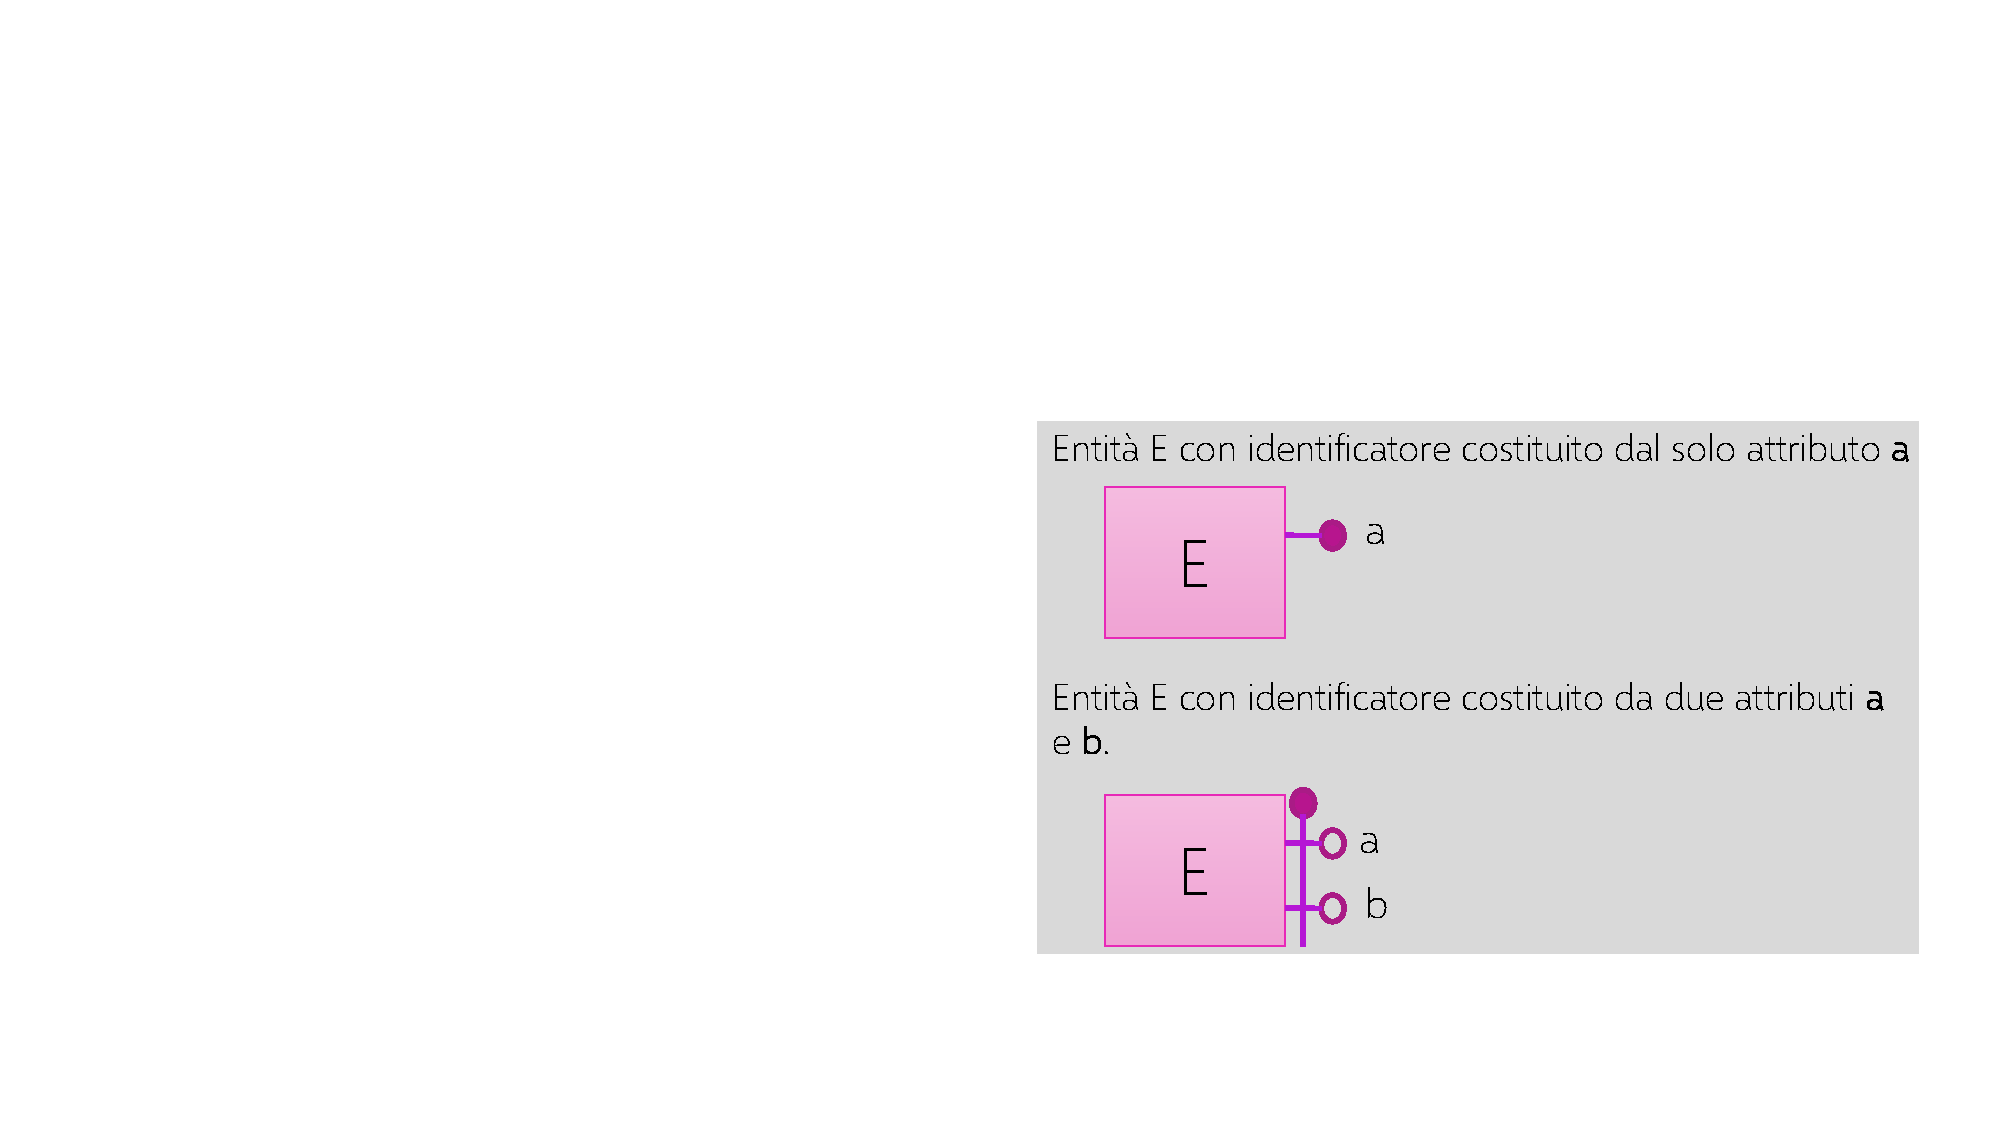
\includegraphics[width=0.7\textwidth]{img/identificatore_def.pdf}
		\caption{Sintassi grafica dell'identificatore.}
	\end{figure}

	\newpage
	
	\subsubsection{Generalizzazioni}
	
	\textcolor{Red3}{\textbf{Definizione.}} Sono i legami logici tra un'entità $E$, chiamata \textbf{entità \underline{genitore}}, e una o più entità $E_{1}, ..., E_{n}$, dette \textbf{entità \underline{figlie}}, di cui $E$ è più generale, nel senso che le comprende come caso particolare. Quindi, si dice che $E$ è \textbf{\underline{generalizzazione}} di $E_{1}, ..., E_{n}$ e che le entità $E_{1}, ..., E_{n}$ sono \textbf{\underline{specializzazioni}} dell'entità $E$.
	
	\textbf{Per esempio}, l'entità \dquotes{Persona} è una generalizzazione delle entità \dquotes{Uomo e Donna}. Invece, \dquotes{Professionista} è una generalizzazione delle entità \dquotes{Ingegnere, Medico e Avvocato}.\newline
	
	\noindent
	\textbf{\underline{Proprietà.}}
	
	\begin{itemize}
		\item \textbf{Ogni occorrenza di un'entità figlia è anche un'occorrenza dell'entità genitore}. Per esempio, una occorrenza dell'entità \dquotes{Avvocato} è anche una occorrenza dell'entità \dquotes{Professionista}.
		
		\item \textbf{Ogni proprietà dell'entità genitore} (come attributi, identificatori, relazioni e altre generalizzazioni) \textbf{è anche una proprietà delle entità figlie}. Per esempio, se l'entità \dquotes{Persona} ha attributi \dquotes{Cognome ed Età}, anche le entità \dquotes{Uomo} e \dquotes{Donna} possiedono questi attributi.
	\end{itemize}

	\noindent
	\textbf{\underline{Classificazioni.}} Le generalizzazioni possono essere classificate:
	
	\begin{itemize}
		\item \textbf{\underline{Totale.}} Ogni occorrenza dell'entità genitore è una occorrenza di almeno una dell'entità figlie. Se non è così, la generalizzazione è \textbf{\underline{parziale}};
		
		\item \textbf{\underline{Esclusiva.}} Ogni occorrenza dell'entità genitore è al massimo un'occorrenza di una delle entità figlie. Se non è così, la generalizzazione è \textbf{\underline{sovrapposta}}.
	\end{itemize}

	\noindent
	In generale, una stessa entità può essere coinvolta in più generalizzazioni diverse. Possono esserci \textbf{generalizzazioni su più livelli}: in questo caso si parla di \textbf{\underline{gerarchia}} di generalizzazioni. Infine, una \textbf{generalizzazione può avere una sola entità figlia}: in questo caso si parla di \textbf{\underline{sottoinsieme}}.
	
	\newpage
	
	\noindent
	\textcolor{Green4}{\textbf{Sintassi grafica.}} Non è difficile da comprendere, ma si presti attenzione a $\left(x, y\right)$. Esse indicano il \textbf{tipo di generalizzazione}:
	
	\begin{itemize}
		\item $\left[t,e\right] \rightarrow$ totale ed esclusiva;
		
		\item $\left[t,s\right] \rightarrow$ totale e sovrapposta;
		
		\item $\left[p,e\right] \rightarrow$ parziale ed esclusiva;
		
		\item $\left[p,s\right] \rightarrow$ parziale e sovrapposta.
	\end{itemize}

	\begin{figure}[!htp]
		\centering
		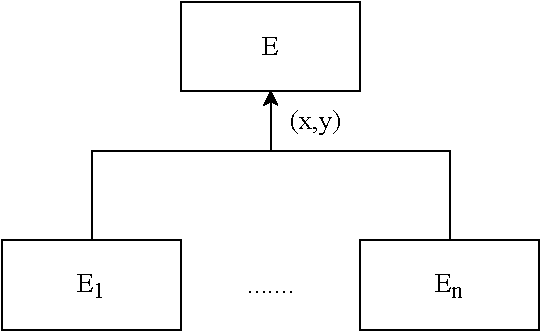
\includegraphics[width=0.6\textwidth]{img/generalizzazione_sintassi.pdf}
		\caption{Sintassi grafica della generalizzazione.}
	\end{figure}

	\newpage
	
	\section{Progettazione concettuale}
	
	\subsection{Strategie di progetto}
	
	Lo sviluppo di uno schema concettuale a partire dalle sue specifiche può essere considerato un processo di ingegnerizzazione.
	
	\subsubsection{Strategia top-down}
	
	Lo schema concettuale viene prodotto mediante una serie di raffinamenti successivi a partire da uno schema iniziale che descrive tutte le specifiche con pochi concetti molto astratti. Lo schema viene poi via via raffinato mediante opportune trasformazioni che aumentano il dettaglio dei vari concetti presenti.\newline
	
	\noindent
	In sintesi:
	
	\begin{enumerate}
		\item \textbf{Fase 1}, si considerano le \emph{specifiche globalmente} e si produce uno schema iniziale completo ma con \emph{pochi concetti} molto \emph{astratti};
		
		\item \textbf{Fase 2}, si esegue un \emph{raffinamento} dei concetti astratti fino ad arrivare allo schema concettuale \emph{completo} in ogni \emph{dettaglio}.
	\end{enumerate}

	\noindent
	\textcolor{Green4}{\textbf{\emph{Vantaggio:}}} il progettista può \textbf{descrivere inizialmente tutte le specifiche dei dati trascurandone i dettagli}, per \textbf{poi entrare nel merito} di un concetto alla volta.\newline
	
	\noindent
	\textcolor{Red3}{\textbf{\emph{Svantaggio:}}} si deve \textbf{possedere} una \textbf{visione globale e astratta} di \emph{tutte} le componenti del sistema, ma solitamente è difficile.
	
	\newpage
	
	\subsubsection{Strategia bottom-up}
	
	Le specifiche iniziali sono suddivise in componenti via via sempre più piccole, fino a quando queste componenti descrivono un frammento elementare della realtà di interesse. A questo punto, le varie componenti vengono rappresentate da semplici schemi concettuali che possono consistere anche in singoli concetti. I vari schemi così ottenuti vengono poi fusi fino a giungere attraverso una completa integrazione di tutte le componenti, allo schema concettuale finale.
	
	La \textbf{differenza rispetto alla strategia top-down} è che i vari concetti presenti nello schema finale vengono via via introdotti durante le varie fasi.\newline
	
	\noindent
	In sintesi:
	
	\begin{enumerate}
		\item \textbf{Fase 1}, si \emph{decompongono} le specifiche iniziali in \emph{parti elementari}, ovvero in frasi che descrivono lo stesso concetto;
		
		\item \textbf{Fase 2}, si \emph{generano} gli schemi per tutte le parti elementari individuate;
		
		\item \textbf{Fase 3}, si \emph{fondono} gli schemi (introducendo altri costrutti del modello E-R) in modo da \emph{integrare} tutti gli schemi componenti e generare lo \emph{schema finale}.
	\end{enumerate}

	\noindent
	\textcolor{Green4}{\textbf{\emph{Vantaggio:}}} questa strategia si adatta a una \textbf{decomposizione del problema in componenti più semplici}, facilmente individuabili, il cui progetto può essere affrontato anche da progettisti diversi.\newline
	
	\noindent
	\textcolor{Red3}{\textbf{\emph{Svantaggio:}}} vengono richieste delle operazioni di \textbf{integrazione di schemi concettuali diversi} che, nel caso di schemi complessi, presentano \textbf{quasi sempre grosse difficoltà}.
	
	\newpage
	
	\subsubsection{Strategia inside-out}
	
	Si individuano inizialmente solo alcuni concetti importanti e poi si procede, a partire da questi, a \dquotes{macchia d'olio}. Si rappresentano cioè prima i concetti in relazione con i concetti iniziali, per poi muoversi verso quelli più lontani attraverso una \dquotes{navigazione} tra le specifiche.\newline
	
	\noindent
	In sintesi:
	
	\begin{enumerate}
		\item \textbf{Fase 1}, si \emph{individua} nelle specifiche alcuni \emph{concetti importanti}, chiamati concetti guida;
		
		\item \textbf{Fase 2}, si \emph{generano} gli schemi per i concetti guida;
		
		\item \textbf{Fase 3}, si \emph{fondono} gli schemi precedenti e si genera lo \emph{schema finale}.
	\end{enumerate}
	
	\noindent
	\textcolor{Green4}{\textbf{\emph{Vantaggio:}}} \textbf{non sono richiesti passi di integrazione}.\newline
	
	\noindent
	\textcolor{Red3}{\textbf{\emph{Svantaggio:}}} è necessario, di volta in volta, \textbf{esaminare tutte le specifiche} per \textbf{individuare concetti non ancora rappresentati} e \textbf{descrivere i nuovi concetti nel dettaglio}.
	
	\newpage
	
	\subsection{Qualità di uno schema concettuale}
	
	L'analisi della qualità dello schema concettuale prodotto può essere suddivisa in diverse fasi:
	
	\begin{itemize}
		\item Correttezza
		\item Completezza
		\item Leggibilità
		\item Minimalità
	\end{itemize}

	\subsubsection{Correttezza}\label{correttezza}

	\textcolor{Red3}{\textbf{\emph{Definizione.}}} Uno schema concettuale è \textbf{corretto} quando \textbf{utilizza propriamente i costrutti} messi a disposizione dal modello concettuale di riferimento.\newline
	
	\noindent
	Gli errori che si possono commettere nello schema concettuale sono principalmente due:
	
	\begin{itemize}
		\item \textcolor{Red3}{\textbf{\emph{Sintattici}}}. Vengono utilizzati costrutti non ammessi. \textcolor{Green4}{Per esempio}, una generalizzazione tra relazioni invece che tra entità.
		
		\item \textcolor{Red3}{\textbf{\emph{Semantici}}}. Vengono usati costrutti senza rispettare la loro definizione. \textcolor{Green4}{Per esempio}, l'uso di una relazione per descrivere il fatto che una entità è specializzazione di un'altra.
	\end{itemize}
	
	\subsubsection{Completezza}\label{completezza}
	
	\textcolor{Red3}{\textbf{\emph{Definizione.}}} Uno schema concettuale è \textbf{completo} quando \textbf{rappresenta tutti i dati} di interesse e quando \textbf{tutte le operazioni possono essere eseguite} a partire dai concetti descritti nello schema.\newline
	
	\noindent
	La completezza è \textbf{possibile verificarla} controllando che tutte le specifiche sui dati siano rappresentate da qualche concetto presente nello schema che stiamo costruendo, e che tutti i concetti coinvolti in un'operazione presente nelle specifiche siano raggiungibili \dquotes{navigando} attraverso lo schema.
	
	\subsubsection{Leggibilità}\label{leggibilità}
	
	\textcolor{Red3}{\textbf{\emph{Definizione.}}} Uno schema concettuale è \textbf{leggibile} quando rappresenta i requisiti in maniera naturale e facilmente comprensibile.\newline
	
	\noindent
	Per garantire questa proprietà è necessario rendere lo schema autoesplicativo, \textcolor{Green4}{per esempio}, mediante una scelta opportuna dei nomi da dare ai concetti. La leggibilità dipende anche da criteri puramente estetici.
	
	\subsubsection{Minimalità}\label{minimalità}
	
	\textcolor{Red3}{\textbf{\emph{Definizione.}}} Uno schema concettuale è \textbf{minimale} quando tutte le specifiche sui dati sono rappresentate una sola volta nello schema.\newline
	
	\noindent
	Uno schema quindi non è minimale quando esistono delle \textbf{ridondanze}, ovvero concetti che possono essere derivati da altri. La minimalità di uno schema si può \textbf{verificare} per ispezione, controllando se esistono concetti che possono essere eliminati dallo schema che stiamo costruendo senza inficiare la sua completezza.
	
	\newpage
	
	\section{Progettazione logica}
	
	\subsection{Fasi della progettazione logica}
	
	L'\textcolor{Red3}{\textbf{obbiettivo}} della progettazione logica è \textbf{produrre uno schema logico che descriva in modo \underline{corretto} ed \underline{efficace} tutte le informazioni contenute nello schema concettuale}.
	
	Le attività principali della progettazione logica sono la riorganizzazione dello schema concettuale e la traduzione in un modello logico:
	
	\begin{itemize}
		\item \textcolor{Red3}{\textbf{\emph{Ristrutturazione dello schema Entità-Relazione}}}: è una fase indipendente dal modello logico scelto e si basa su \textbf{criteri di ottimizzazione} dello schema e di \textbf{semplificazione} della fase successiva. In particolare, le fasi sono:
		\begin{itemize}
			\item Analisi delle ridondanze dovute alla presenza di dati derivabili;
			\item Eliminazione delle generalizzazioni;
			\item Accorpamento/partizionamento di entità e relazioni;
			\item Scelta degli identificatori principali.
		\end{itemize}
	
		\item \textcolor{Red3}{\textbf{\emph{Traduzione verso il modello logico}}}: fa riferimento a uno specifico modello logico (nel nostro caso modello relazionale) e può includere una ulteriore ottimizzazione che si basa sulle caratteristiche del modello logico stesso.
	\end{itemize}
	
	\newpage
	
	\subsection{Traduzione verso il modello logico}
	
	La seconda fase della progettazione logica corrisponde ad una traduzione tra modelli di dati diversi. Si parte da uno schema E-R ristrutturato e si costruisce uno schema logico equivalente, in grado cioè di rappresentare le medesime informazioni.
	
	Si affronta il problema della traduzione caso per caso, iniziando dal caso più generale che ci suggerisce l'idea generale su cui si basa la metodologia di traduzione.
	
	\subsubsection{Entità e attributo opzionale}
	
	L'\textcolor{Red3}{\textbf{\underline{entità}}} si rappresenta una relazione (lettera maiuscola) con lo stesso nome avente per attributi (lettere tra parentesi) i medesimi attributi dell'entità e per chiave il suo identificatore.
	
	\begin{figure}[!htp]
		\centering
		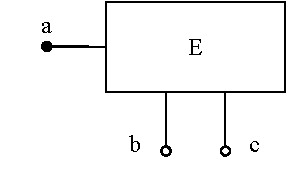
\includegraphics[width=0.4\textwidth]{img/relazionale_entita.pdf}
		\caption{Modello E-R di un'entità.}
	\end{figure}

	\noindent
	Relativo modello relazionale:
	
	\begin{equation*}
		\textbf{E}\left(a,b,c\right)
	\end{equation*}

	\noindent
	Invece, un possibile \textcolor{Red3}{\textbf{\underline{attributo nullo}}} si rappresenta inserendo un asterisco.
	
	\begin{figure}[!htp]
		\centering
		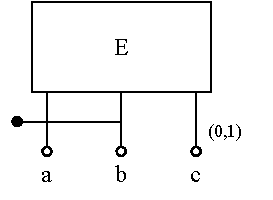
\includegraphics[width=0.4\textwidth]{img/relazionale_attributo_nullo.pdf}
		\caption{Modello E-R di un possibile attributo nullo.}
	\end{figure}
	
	\noindent
	Relativo modello relazionale:
	
	\begin{equation*}
		\textbf{E}\left(\underline{a,b},c^{*}\right)
	\end{equation*}

	\newpage
	
	\subsubsection{Relazione uno a molti}
	
	La \textcolor{Red3}{\textbf{\underline{relazione uno a molti}}} è caratterizzata dal fatto che un'entità è in relazione con un'altra con cardinalità $\left(1,1\right)$ e la corrispondente entità ha cardinalità $\left(x,N\right)$ ($x$ può essere qualsiasi valore minimo).
	
	\begin{figure}[!htp]
		\centering
		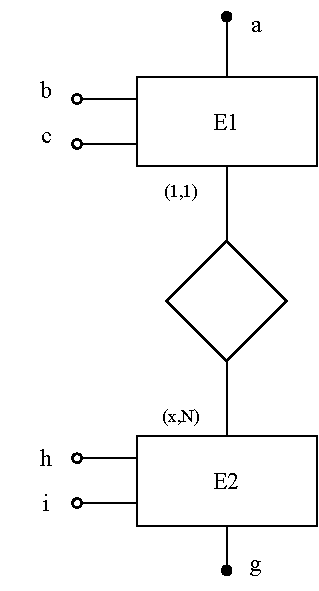
\includegraphics[width=0.5\textwidth]{img/relazionale_uno_a_molti.pdf}
		\caption{Modello E-R di una relazione uno a molti.}
	\end{figure}
	
	\noindent
	Relativo modello relazionale:
	
	\begin{figure}[!htp]
		\centering
		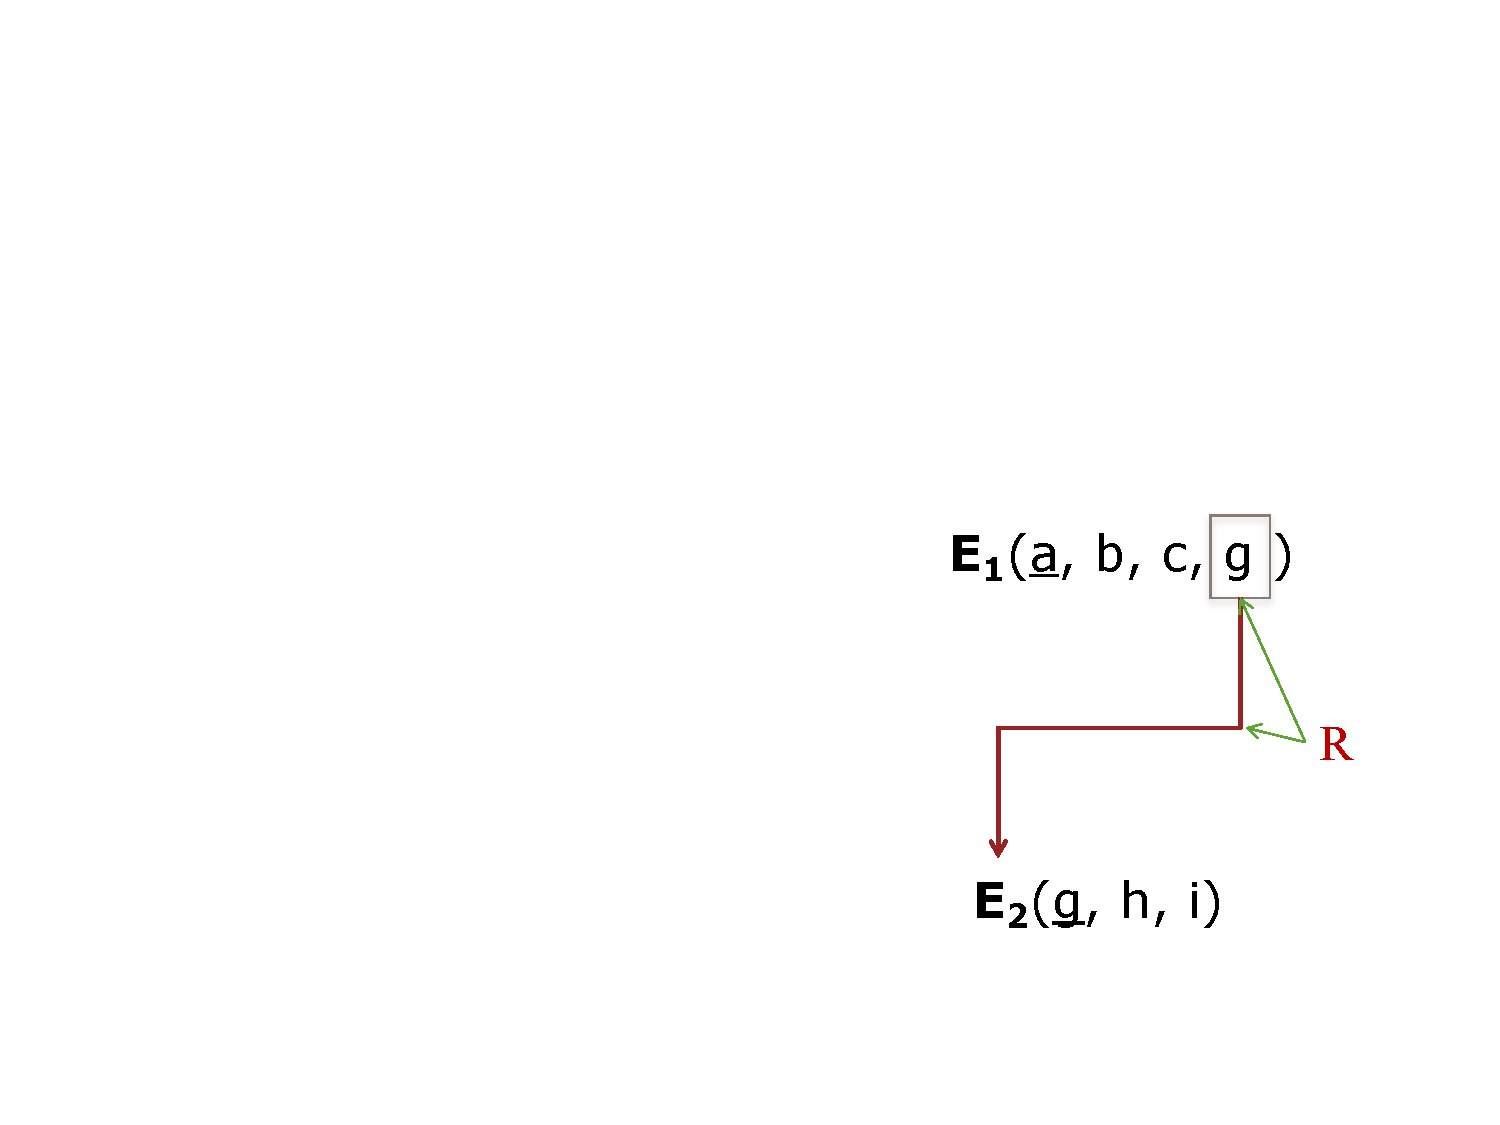
\includegraphics[width=0.3\textwidth]{img/relazionale_uno_a_molti2.pdf}
	\end{figure}

	\newpage
	
	\subsubsection{Relazione uno a uno}
	
	La \textcolor{Red3}{\textbf{\underline{relazione uno a uno}}} è caratterizzata dal fatto che entrambe le entità hanno cardinalità $\left(1,1\right)$.
	
	\begin{figure}[!htp]
		\centering
		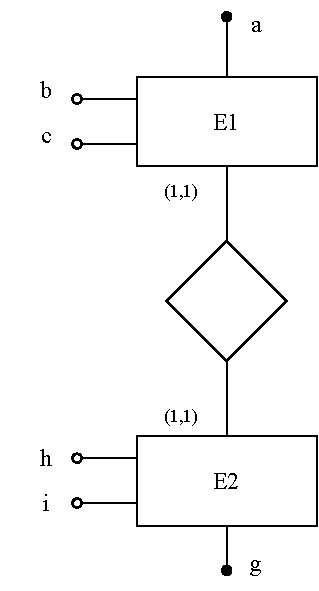
\includegraphics[width=0.5\textwidth]{img/relazionale_uno_a_uno.pdf}
		\caption{Modello E-R di una relazione uno a uno.}
	\end{figure}
	
	\noindent
	Relativo modello relazionale:
	
	\begin{figure}[!htp]
		\centering
		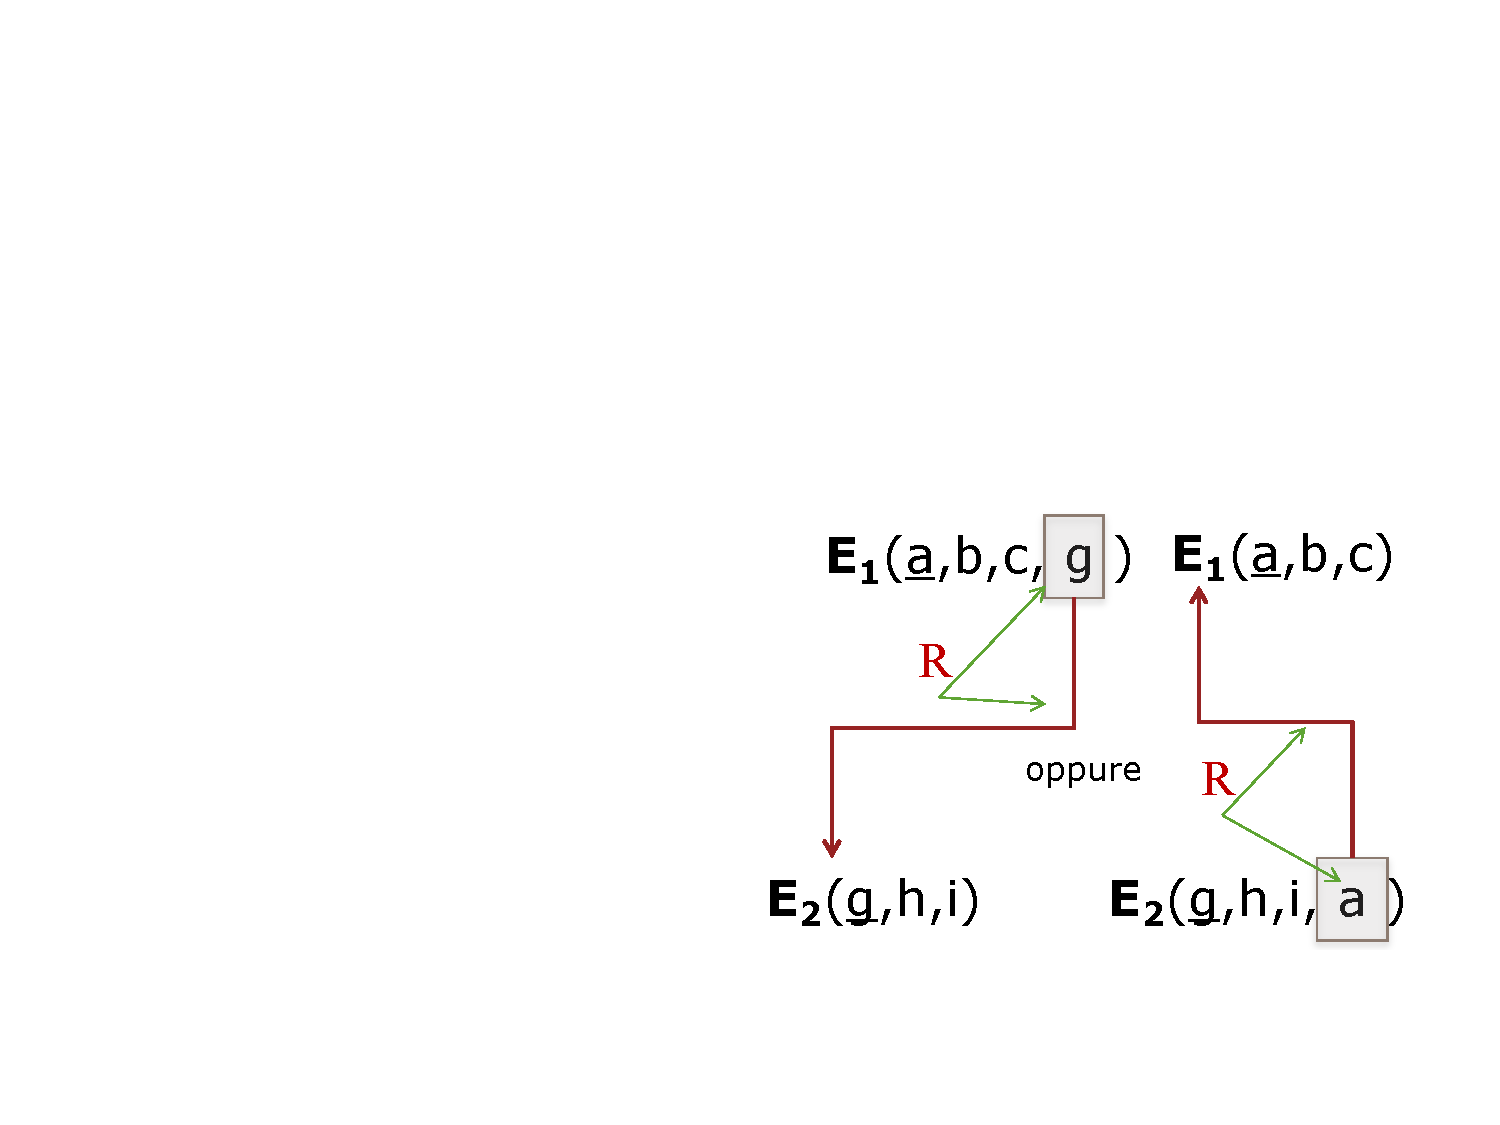
\includegraphics[width=0.4\textwidth]{img/relazionale_uno_a_uno2.pdf}
	\end{figure}

	\newpage
	
	\subsubsection{Relazione molti a molti}
	
	La \textcolor{Red3}{\textbf{\underline{relazione molti a molti}}} è caratterizzata dal fatto che entrambe le entità hanno cardinalità $\left(x,N\right)$ ($x$ può essere qualsiasi valore minimo).
	
	\begin{figure}[!htp]
		\centering
		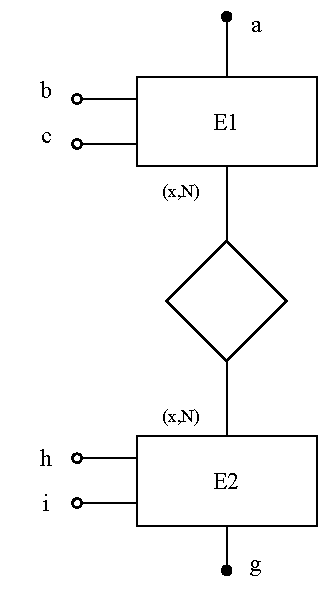
\includegraphics[width=0.5\textwidth]{img/relazionale_molti_a_molti.pdf}
		\caption{Modello E-R di una relazione molti a molti.}
	\end{figure}
	
	\noindent
	Relativo modello relazionale:
	
	\begin{figure}[!htp]
		\centering
		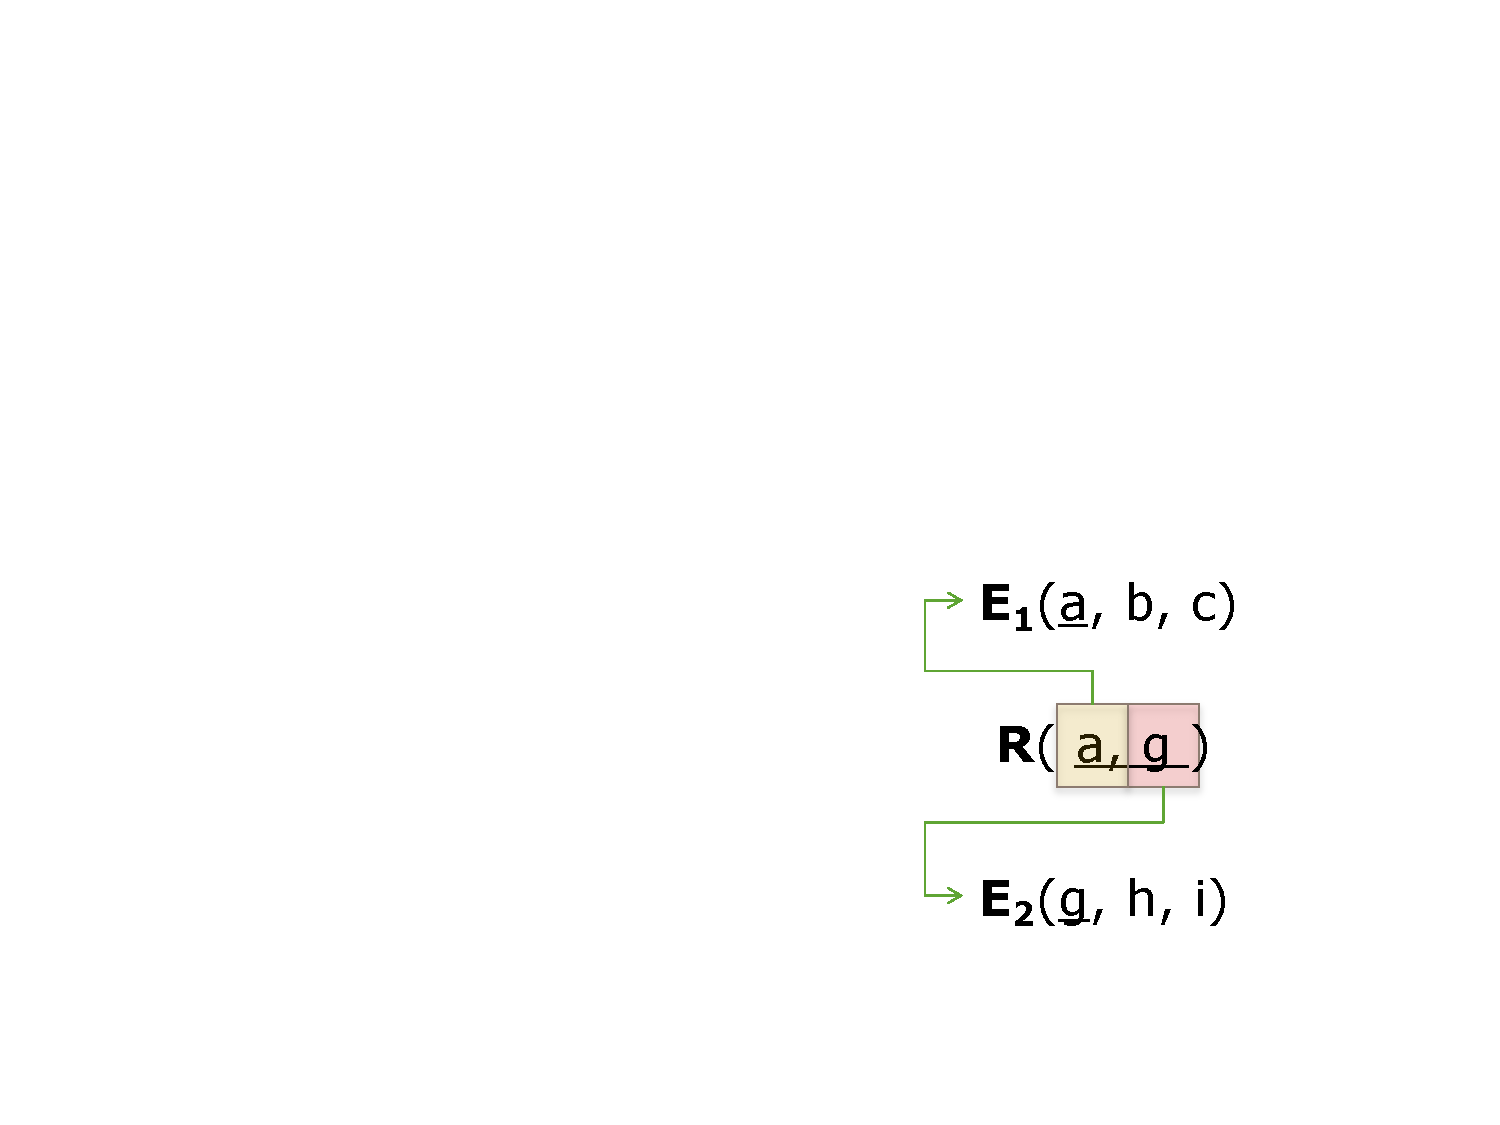
\includegraphics[width=0.2\textwidth]{img/relazionale_molti_a_molti2.pdf}
	\end{figure}

	\newpage
	
	\subsubsection{Relazione uno a molti (identificatore esterno)}
	
	La \textcolor{Red3}{\textbf{\underline{relazione uno a molti con identificatore esterno}}} è caratterizzata dal fatto che un'entità ha cardinalità $\left(1,1\right)$ e l'altra entità ha $\left(x,N\right)$ ($x$ può essere qualsiasi valore minimo).
	
	\begin{figure}[!htp]
		\centering
		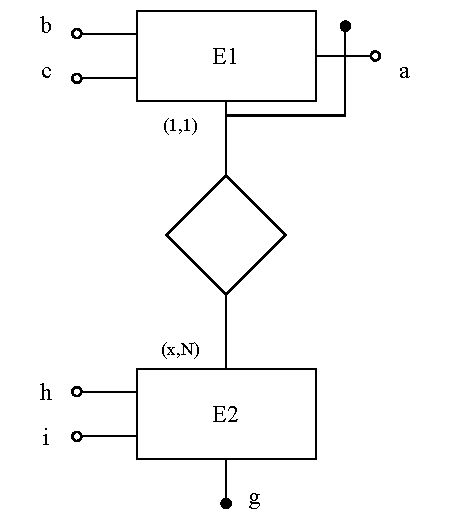
\includegraphics[width=0.5\textwidth]{img/relazionale_uno_a_molti_id_esterno.pdf}
		\caption{Modello E-R di una relazione molti a molti.}
	\end{figure}
	
	\noindent
	Relativo modello relazionale:
	
	\begin{figure}[!htp]
		\centering
		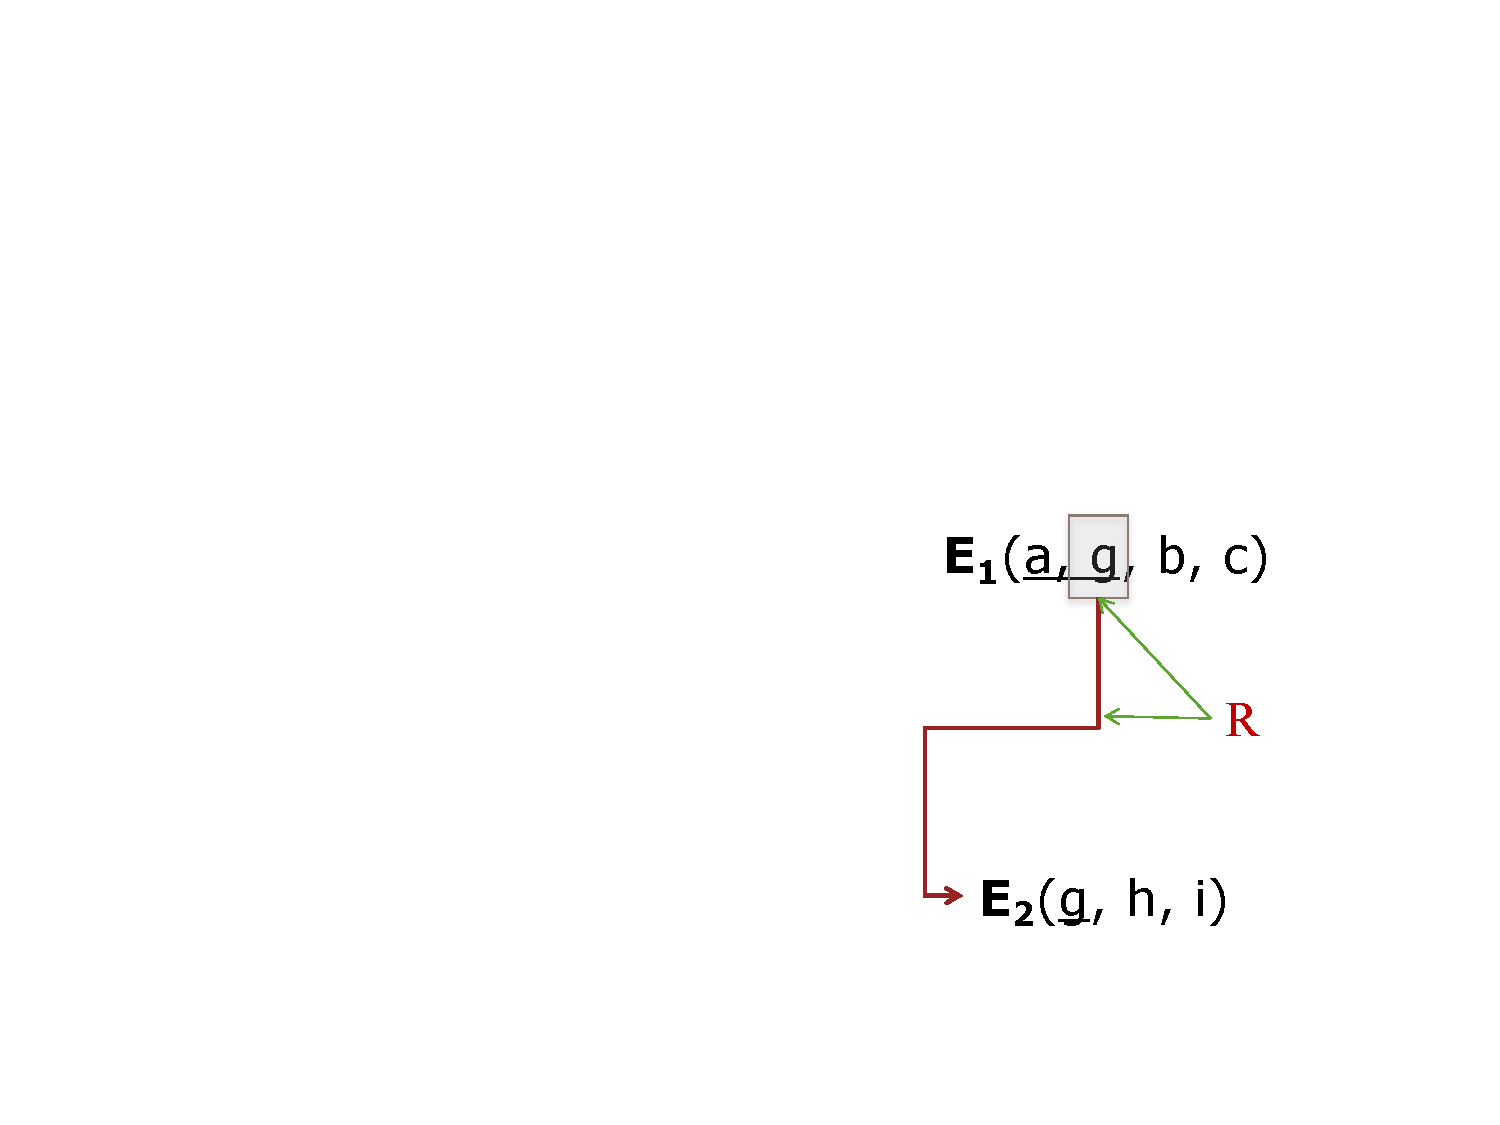
\includegraphics[width=0.2\textwidth]{img/relazionale_uno_a_molti_id_esterno2.pdf}
	\end{figure}

	\newpage
	
	\subsubsection{Relazione uno a molti (attributo sulla relazione)}
	
	La \textcolor{Red3}{\textbf{\underline{relazione uno a molti con un attributo sulla relazione}}} è caratterizzata dal fatto che un'entità ha cardinalità $\left(1,1\right)$, l'altra entità ha $\left(x,N\right)$ ($x$ può essere qualsiasi valore minimo) e un attributo è presente nella relazione.
	
	\begin{figure}[!htp]
		\centering
		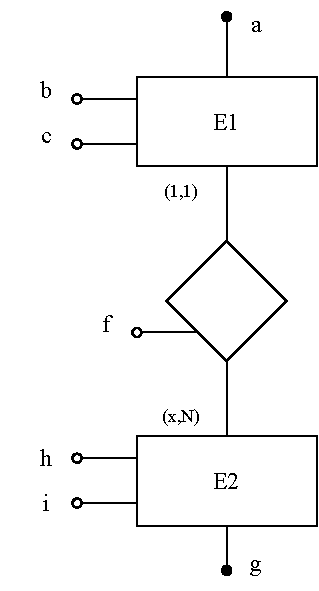
\includegraphics[width=0.4\textwidth]{img/relazionale_uno_a_molti_att_relazione.pdf}
		\caption{Modello E-R di una relazione uno a molti con un attributo sulla relazione esterno.}
	\end{figure}
	
	\noindent
	Relativo modello relazionale:
	
	\begin{figure}[!htp]
		\centering
		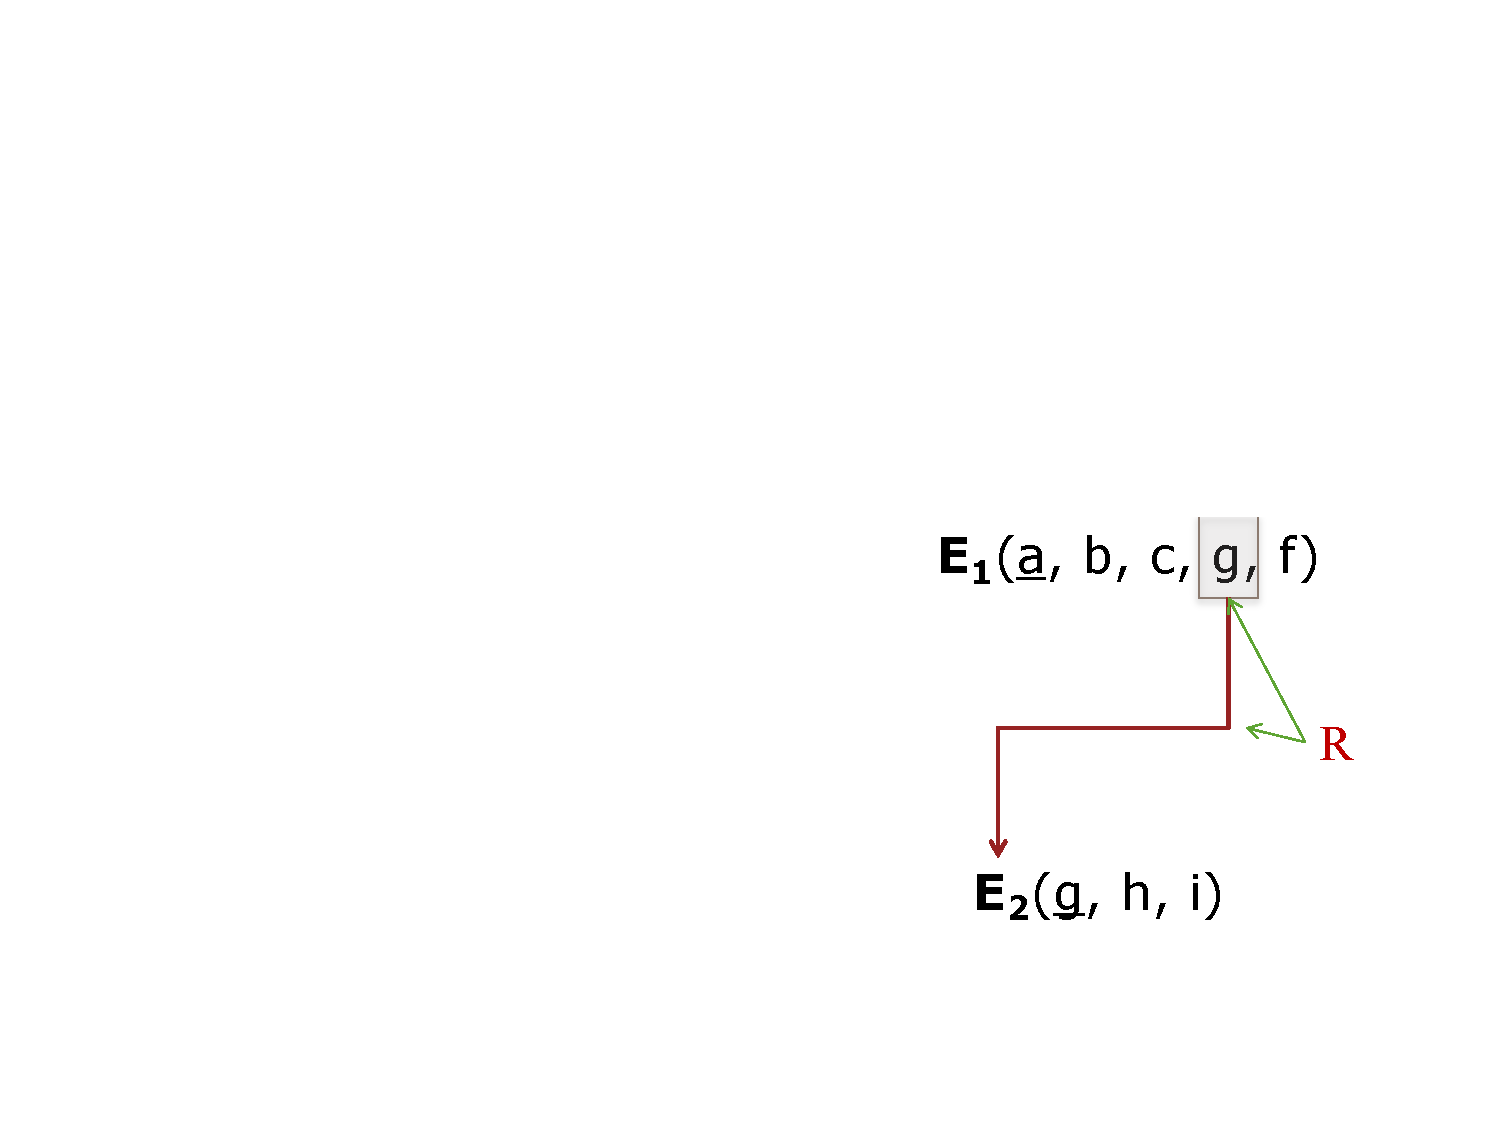
\includegraphics[width=0.2\textwidth]{img/relazionale_uno_a_molti_att_relazione2.pdf}
	\end{figure}

	\newpage
	
	\subsubsection{Relazione uno a uno (una cardinalità minima a zero)}
	
	La \textcolor{Red3}{\textbf{\underline{relazione uno a uno con una cardinalità minima uguale a zero}}} è caratterizzata dal fatto che un'entità ha cardinalità $\left(0,1\right)$, l'altra entità ha $\left(1,1\right)$.
	
	\begin{figure}[!htp]
		\centering
		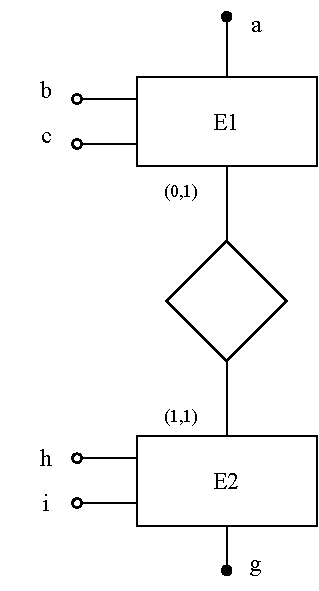
\includegraphics[width=0.4\textwidth]{img/relazionale_uno_a_uno_card_minima_0.pdf}
		\caption{Modello E-R di una relazione uno a uno con una cardinalità minima uguale a zero.}
	\end{figure}
	
	\noindent
	Relativo modello relazionale:
	
	\begin{figure}[!htp]
		\centering
		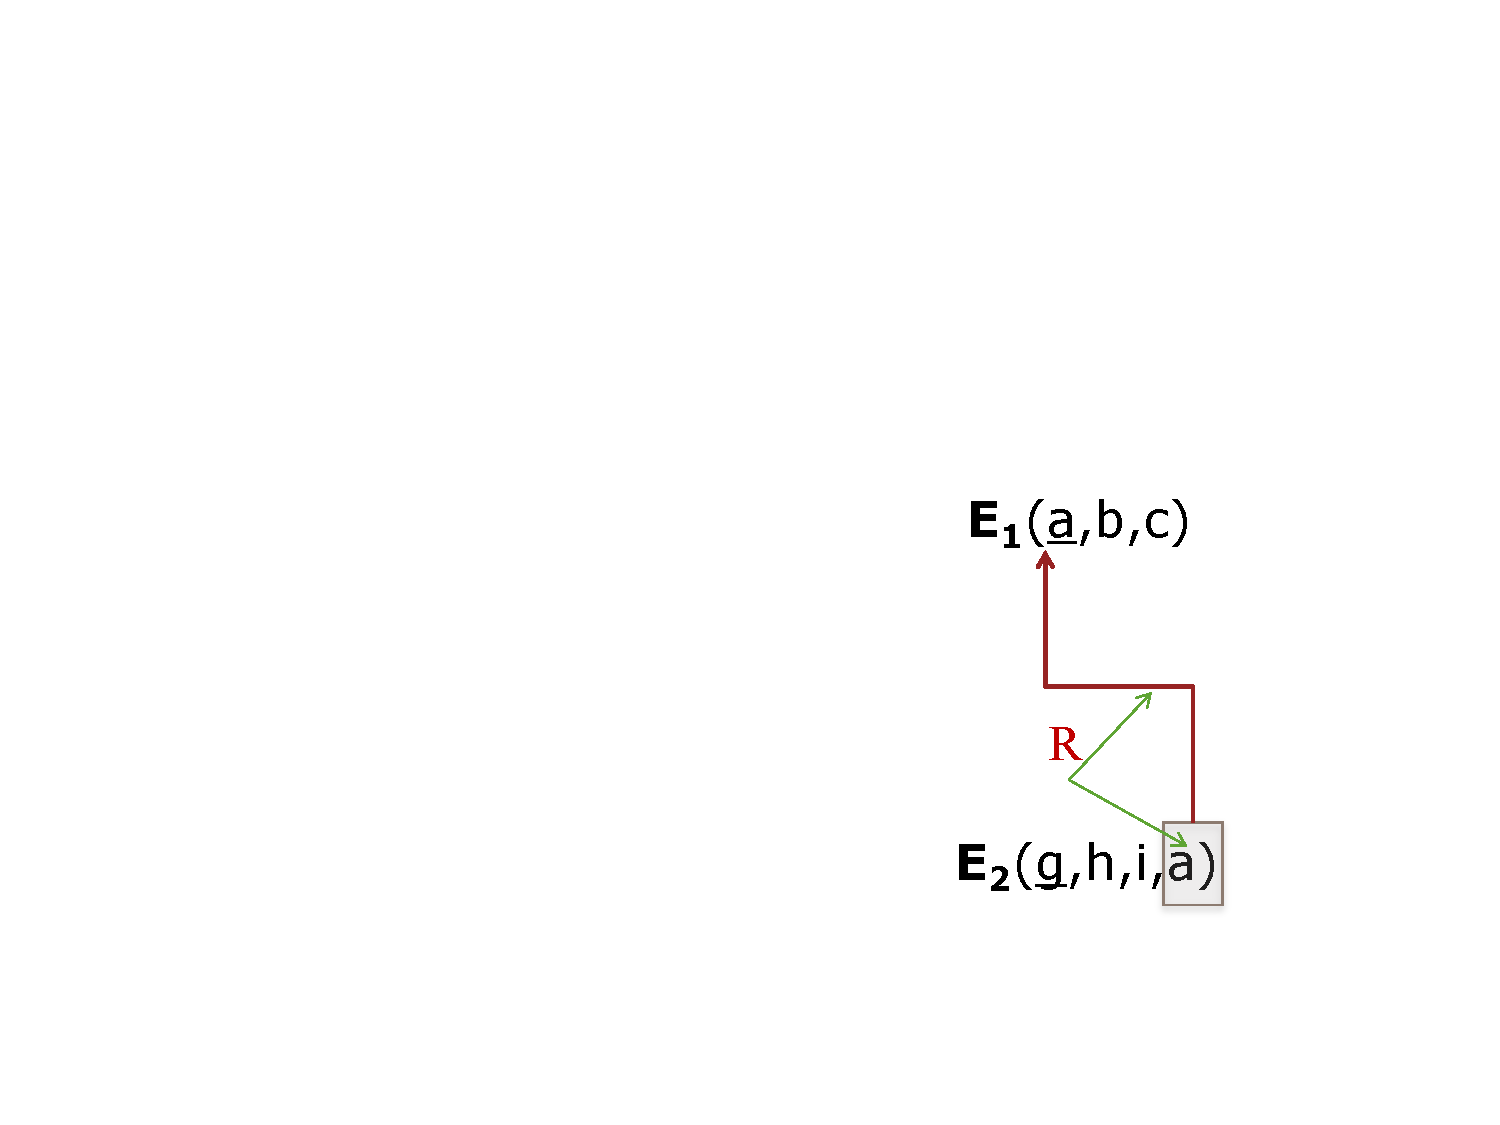
\includegraphics[width=0.2\textwidth]{img/relazionale_uno_a_uno_card_minima_02.pdf}
	\end{figure}

	\newpage
	
	\subsubsection{Relazione uno a uno (entrambe cardinalità minima a zero)}
	
	La \textcolor{Red3}{\textbf{\underline{relazione uno a uno con entrambe le cardinalità minima uguale a zero}}} è caratterizzata dal fatto che un'entità ha cardinalità $\left(0,1\right)$, l'altra entità ha $\left(0,1\right)$.
	
	\begin{figure}[!htp]
		\centering
		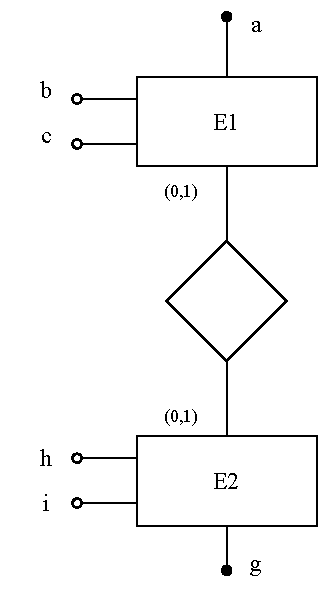
\includegraphics[width=0.4\textwidth]{img/relazionale_uno_a_uno_card_minime_0.pdf}
		\caption{Modello E-R di una relazione uno a uno con entrambe le cardinalità minima uguale a zero.}
	\end{figure}
	
	\noindent
	Relativo modello relazionale:
	
	\begin{figure}[!htp]
		\centering
		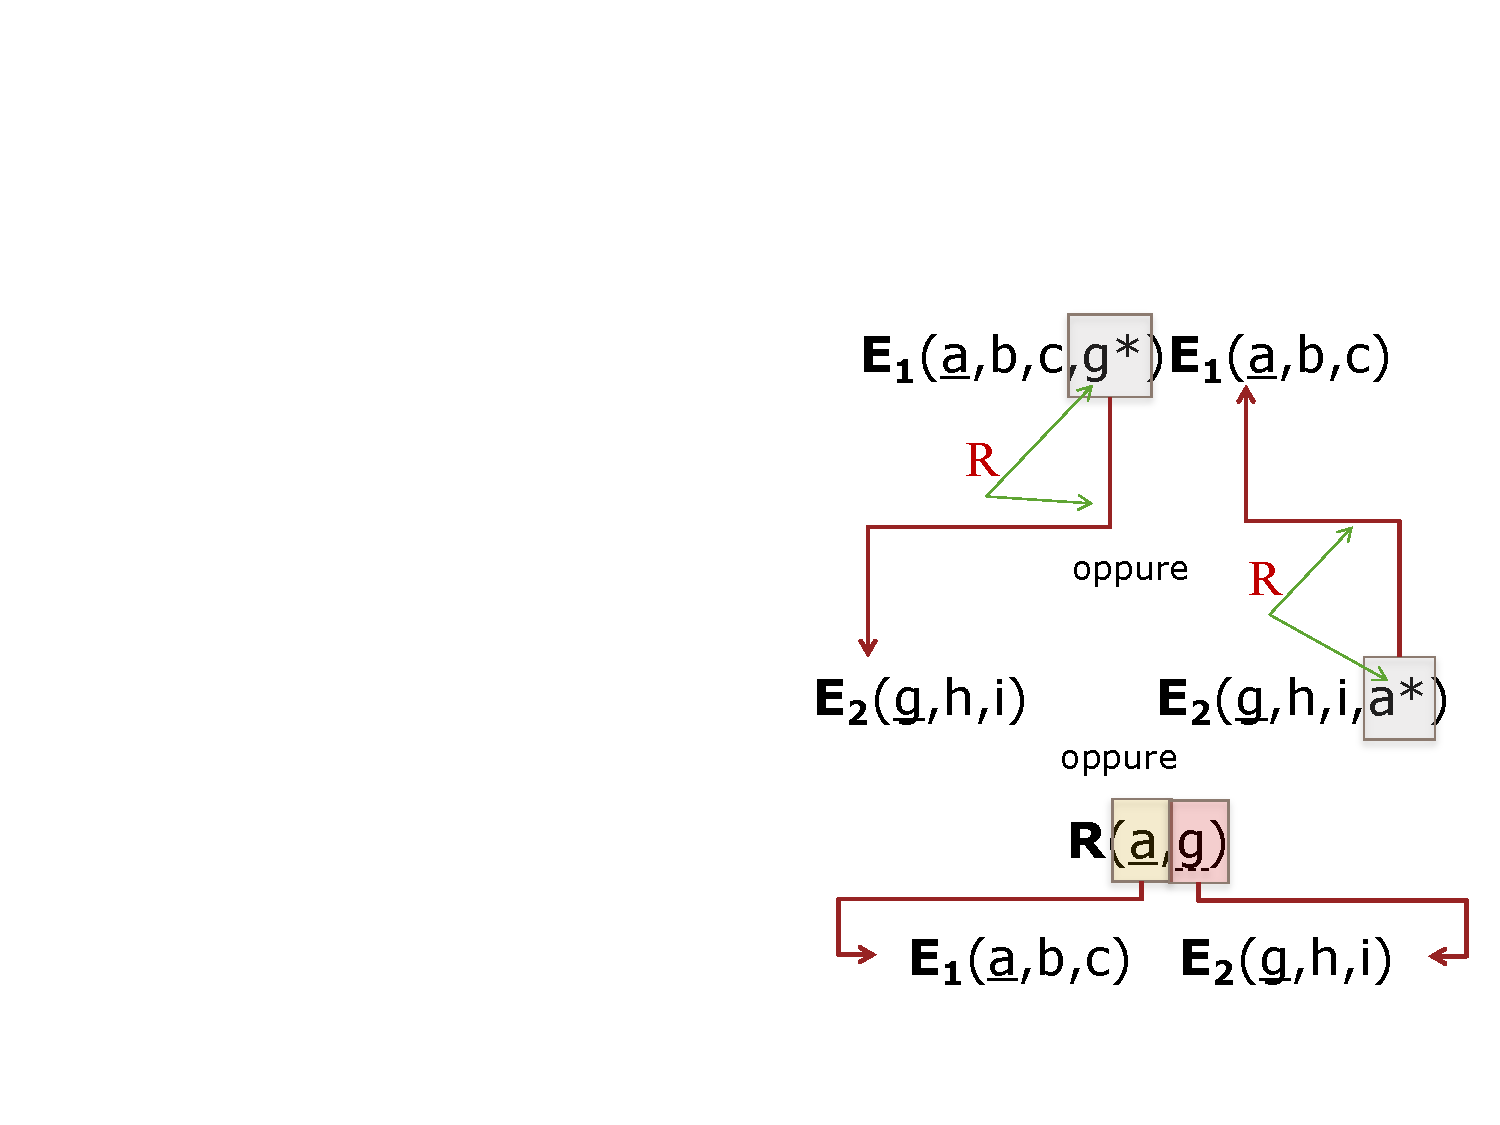
\includegraphics[width=0.4\textwidth]{img/relazionale_uno_a_uno_card_minime_02.pdf}
	\end{figure}

	\newpage
	
	\subsubsection{Relazione molti a molti (attributo sulla relazione)}
	
	La \textcolor{Red3}{\textbf{\underline{relazione molti a molti con un attributo sulla relazione}}} è caratterizzata dal fatto che un'entità ha cardinalità $\left(x,N\right)$, l'altra entità ha $\left(x,N\right)$ ($x$ può essere qualsiasi valore minimo) e un attributo è presente nella relazione.
	
	\begin{figure}[!htp]
		\centering
		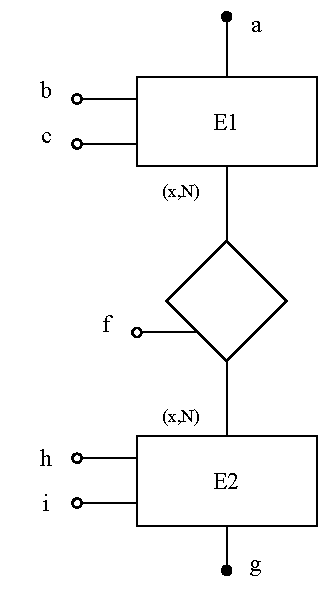
\includegraphics[width=0.4\textwidth]{img/relazionale_molti_a_molti_att_relazione.pdf}
		\caption{Modello E-R di una relazione molti a molti con un attributo sulla relazione esterno.}
	\end{figure}
	
	\noindent
	Relativo modello relazionale:
	
	\begin{figure}[!htp]
		\centering
		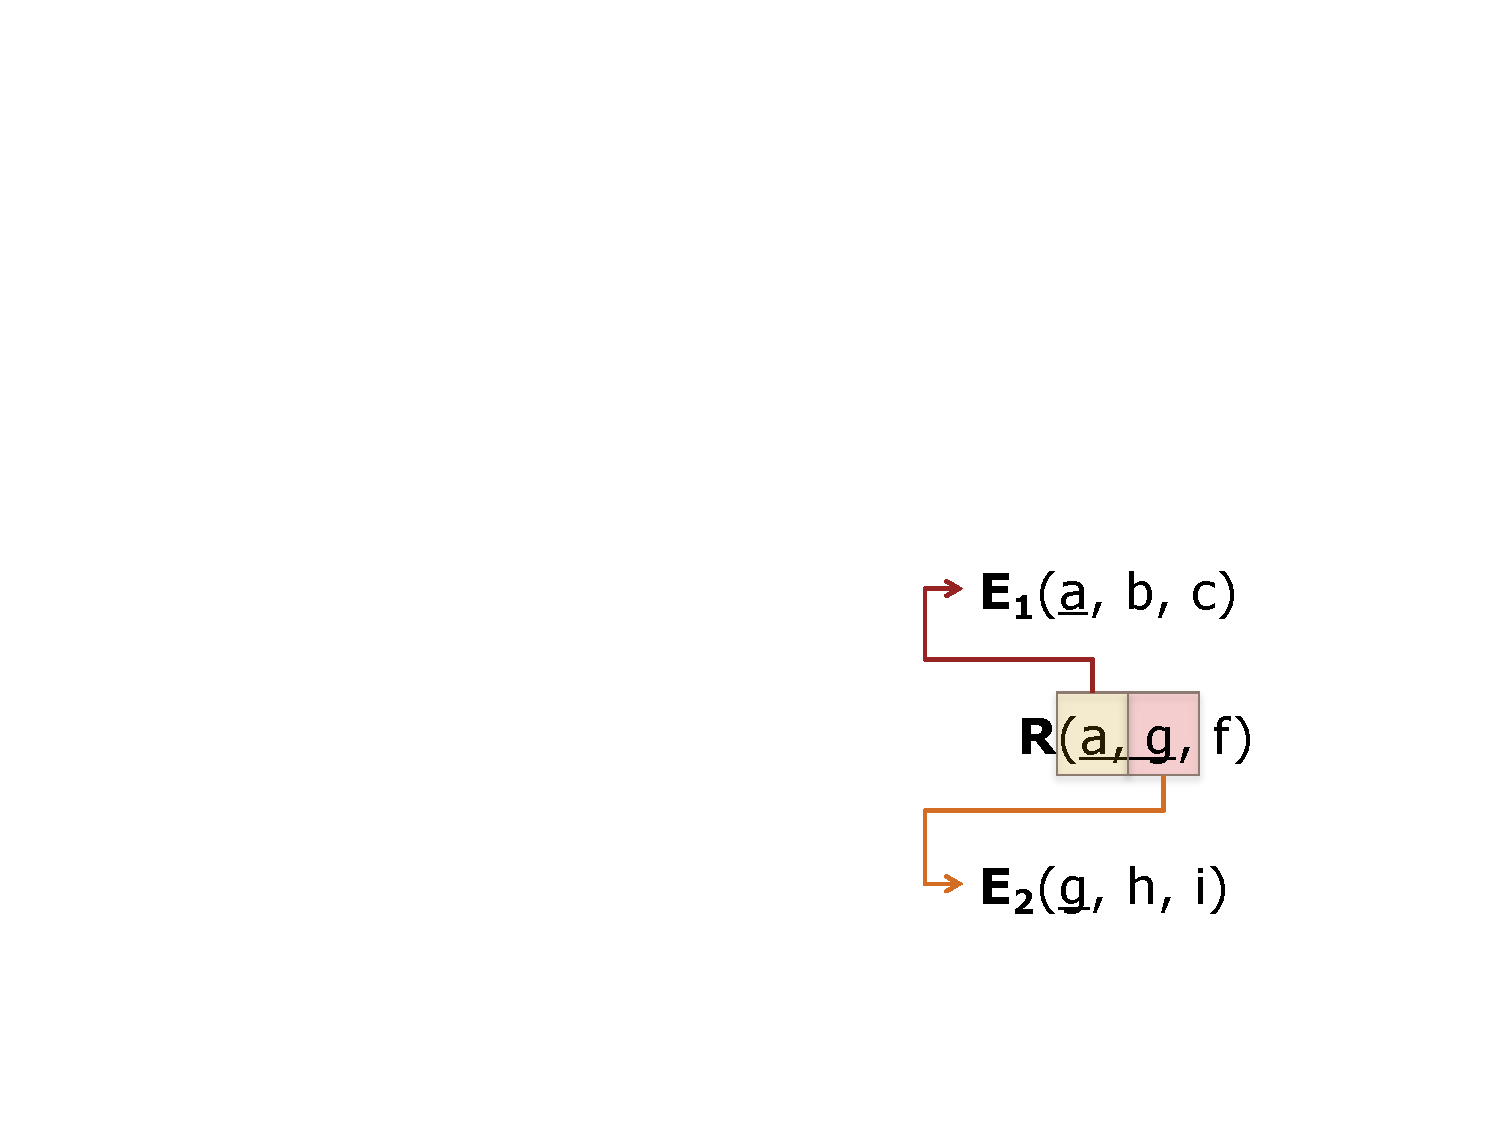
\includegraphics[width=0.25\textwidth]{img/relazionale_molti_a_molti_att_relazione2.pdf}
	\end{figure}

	\newpage
	
	\subsubsection{Relazione molti a molti (identificatori con più attributi)}
	
	La \textcolor{Red3}{\textbf{\underline{relazione molti a molti con identificatori con più attributi}}} è caratterizzata dal fatto che un'entità ha cardinalità $\left(x,N\right)$, l'altra entità ha $\left(x,N\right)$ ($x$ può essere qualsiasi valore minimo) e un attributo è presente nella relazione.
	
	\begin{figure}[!htp]
		\centering
		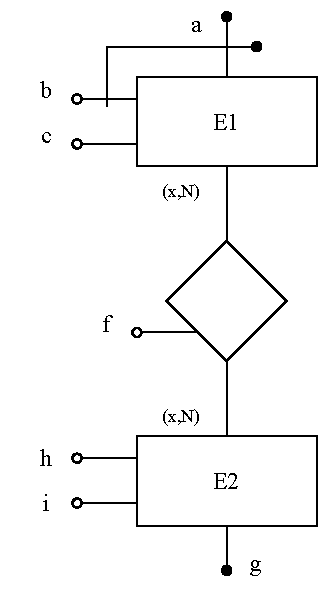
\includegraphics[width=0.4\textwidth]{img/relazionale_molti_a_molti_attributi.pdf}
		\caption{Modello E-R di una relazione molti a molti con identificatori con più attributi.}
	\end{figure}
	
	\noindent
	Relativo modello relazionale:
	
	\begin{figure}[!htp]
		\centering
		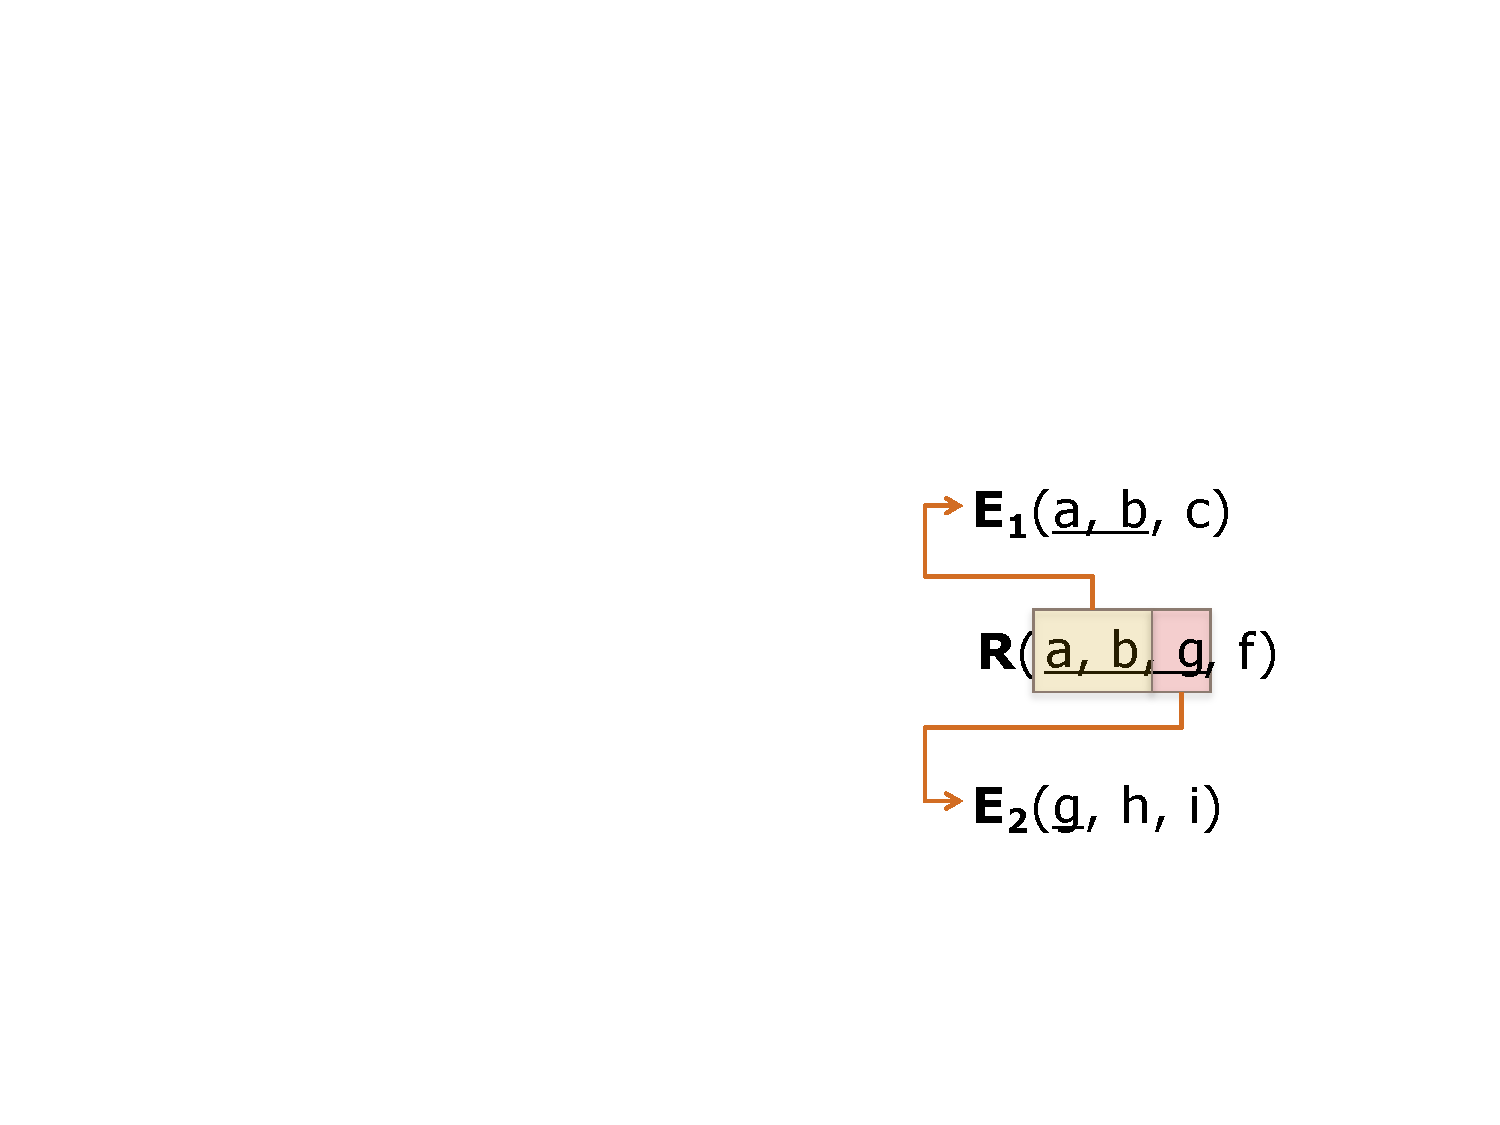
\includegraphics[width=0.25\textwidth]{img/relazionale_molti_a_molti_attributi2.pdf}
	\end{figure}

	\newpage
	
	\subsubsection{Relazione molti a molti (relazione ternaria)}
	
	La \textcolor{Red3}{\textbf{\underline{relazione molti a molti con relazione ternaria}}} è caratterizzata dal fatto che un'entità ha cardinalità $\left(x,N\right)$, l'altra entità ha $\left(x,N\right)$, l'altra entità ancora ha cardinalità $\left(x,N\right)$ ($x$ può essere qualsiasi valore minimo) e un attributo è presente nella relazione.
	
	\begin{figure}[!htp]
		\centering
		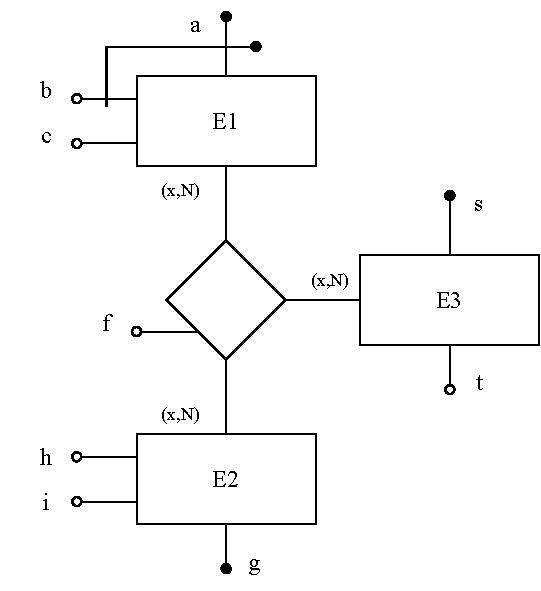
\includegraphics[width=0.6\textwidth]{img/relazionale_molti_a_molti_rel_ternaria.pdf}
		\caption{Modello E-R di una relazione molti a molti con relazione ternaria.}
	\end{figure}
	
	\noindent
	Relativo modello relazionale:
	
	\begin{figure}[!htp]
		\centering
		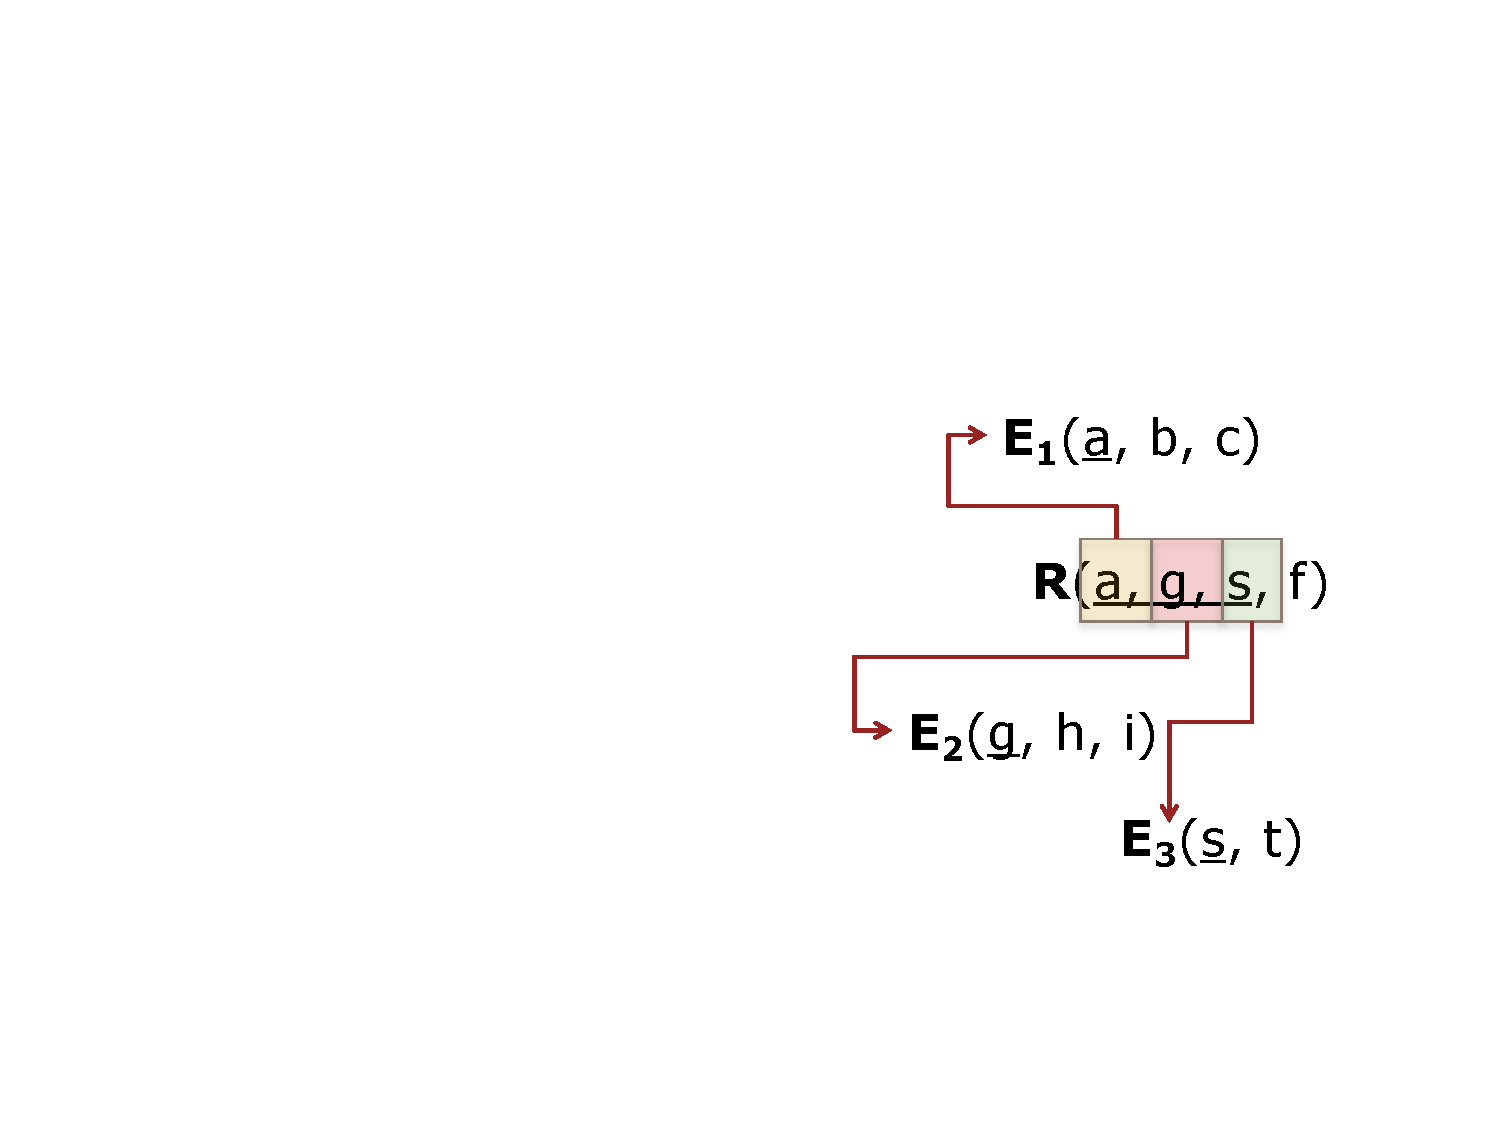
\includegraphics[width=0.32\textwidth]{img/relazionale_molti_a_molti_rel_ternaria2.pdf}
	\end{figure}

	\newpage
	
	\subsubsection{Relazione molti a molti (relazione ternaria e cardinalità uno a uno)}
	
	La \textcolor{Red3}{\textbf{\underline{relazione molti a molti con relazione ternaria e cardinalità uno a uno}}} è caratterizzata dal fatto che un'entità ha cardinalità $\left(1,N\right)$, l'altra entità ha $\left(x,N\right)$, l'altra entità ancora ha cardinalità $\left(x,N\right)$ ($x$ può essere qualsiasi valore minimo) e un attributo è presente nella relazione.
	
	\begin{figure}[!htp]
		\centering
		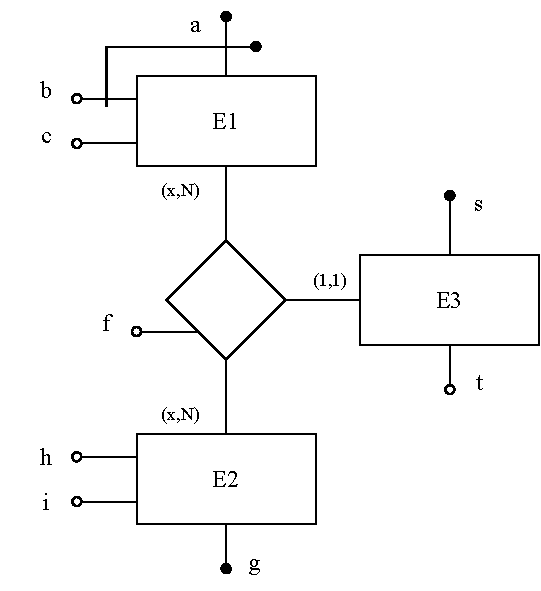
\includegraphics[width=0.6\textwidth]{img/relazionale_molti_a_molti_rel_ternaria_card.pdf}
		\caption{Modello E-R di una relazione molti a molti con relazione ternaria.}
	\end{figure}
	
	\noindent
	Relativo modello relazionale:
	
	\begin{figure}[!htp]
		\centering
		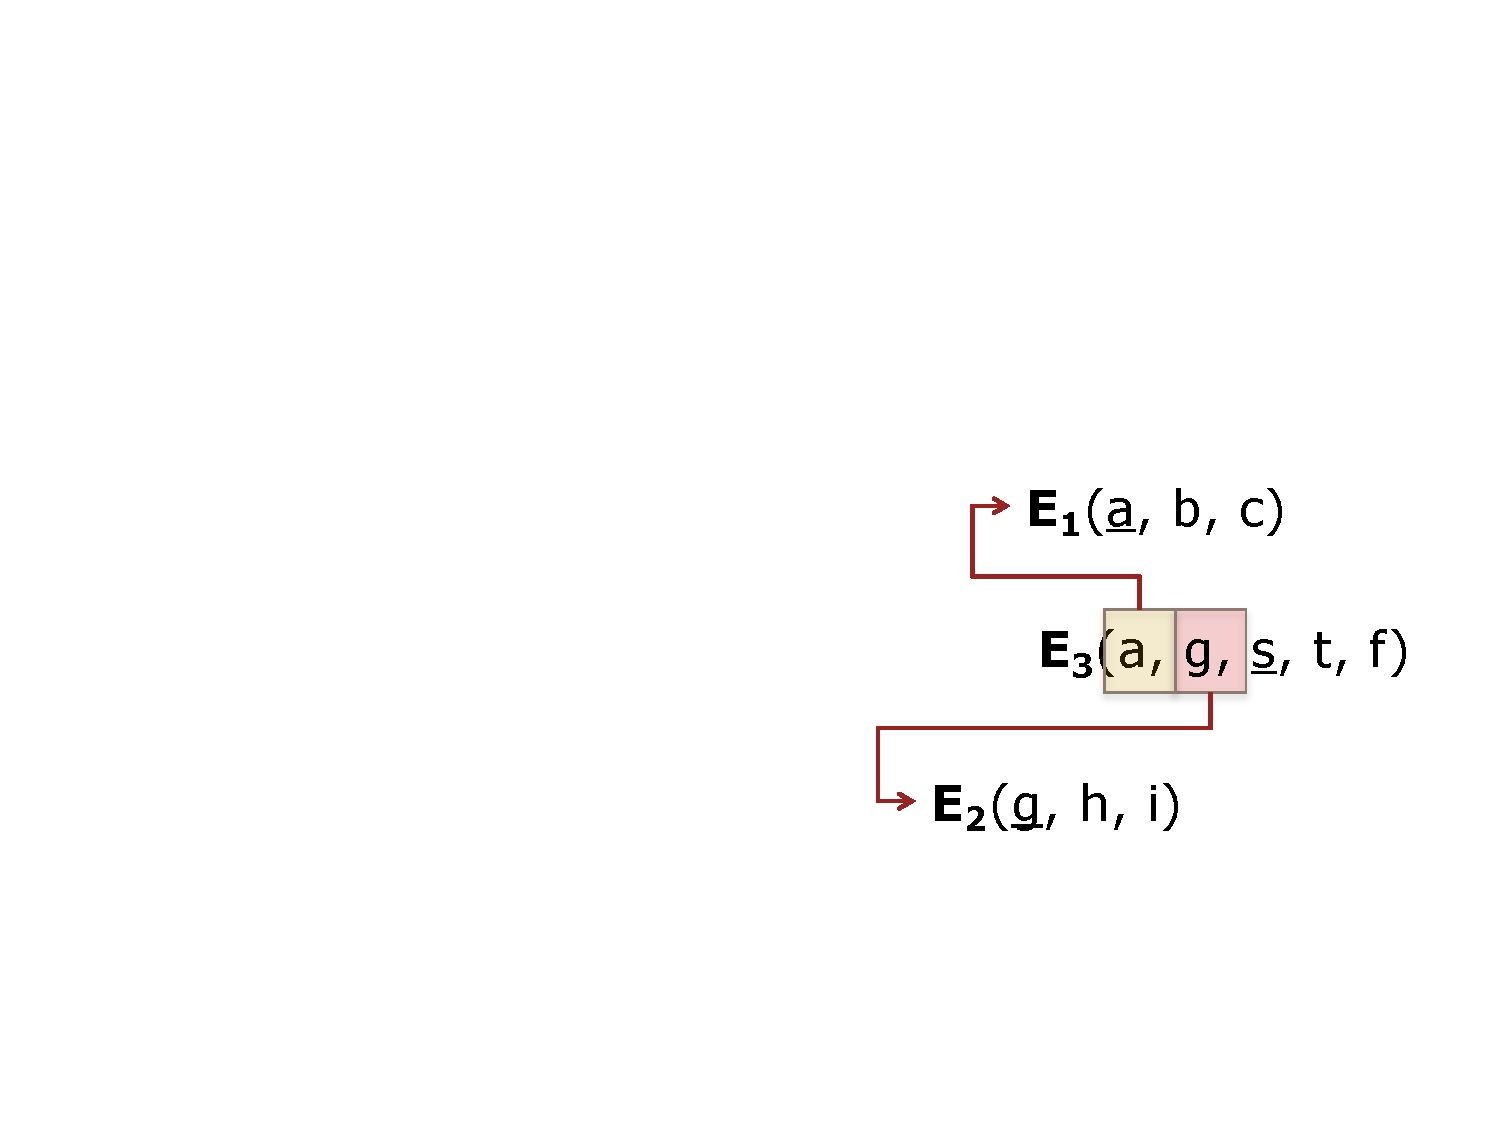
\includegraphics[width=0.4\textwidth]{img/relazionale_molti_a_molti_rel_ternaria_card2.pdf}
	\end{figure}
	
	\newpage
	
	\section{Algebra relazionale}
	
	L'\textcolor{Red3}{\textbf{\underline{algebra relazionale}}} è un linguaggio procedurale, basato su concetti di tipo algebrico. Esso è costituito da un insieme di operatori, definiti su relazioni e che producono ancora relazioni come risultati. I vari operatori sono:
	
	\begin{itemize}
		\item \textbf{Insiemistici}
		\begin{itemize}
			\item \emph{Unione}
			\item \emph{Intersezione}
			\item \emph{Differenza}
		\end{itemize}
	
		\item \textbf{Specifici}
		\begin{itemize}
			\item \emph{Ridenominazione}
			\item \emph{Selezione}
			\item \emph{Proiezione}
		\end{itemize}
		
		\item \textbf{Più importante} \emph{join}
		\begin{itemize}
			\item \emph{Join naturale}
			\item \emph{Prodotto}
			\item \emph{Cartesiano}
			\item \emph{Semijoin}
			\item \emph{Theta-join}
		\end{itemize}
	\end{itemize}

	\noindent
	In altre parole, l'algebra relazione è un insieme di \textbf{operatori} su \textbf{relazioni}. Dato che le relazioni sono insiemi, ha senso definire su di esse gli operatori insiemistici come l'unione, la differenza e l'intersezione
	
	\newpage
	
	\subsection{Insiemistici}

	\subsubsection{Unione}
	
	L'\textcolor{Red3}{\textbf{\underline{unione}}} di due relazioni $r_{1}$ e $r_{2}$ definite sullo stesso insieme di attributi $X$ è indicata con $r_{1} \cup r_{2}$ ed è una relazione ancora su $X$ contenente le tuple che appartengono a $r_{1}$ oppure a $r_{2}$, oppure a entrambe.\newline
	
	\noindent
	La \textbf{cardinalità}, ovvero il numero di tuple contenute nella relazione del risultato:
	
	\begin{equation*}
		\max\left(|r_{1}|, |r_{2}|\right) \le \left|r_{1} \cup r_{2}\right| \le |r_{1}| + |r_{2}|
	\end{equation*}
	
	\noindent
	\textcolor{Green4}{\textbf{\emph{Esempio}}}
	
	\begin{figure}[!htp]
		\centering
		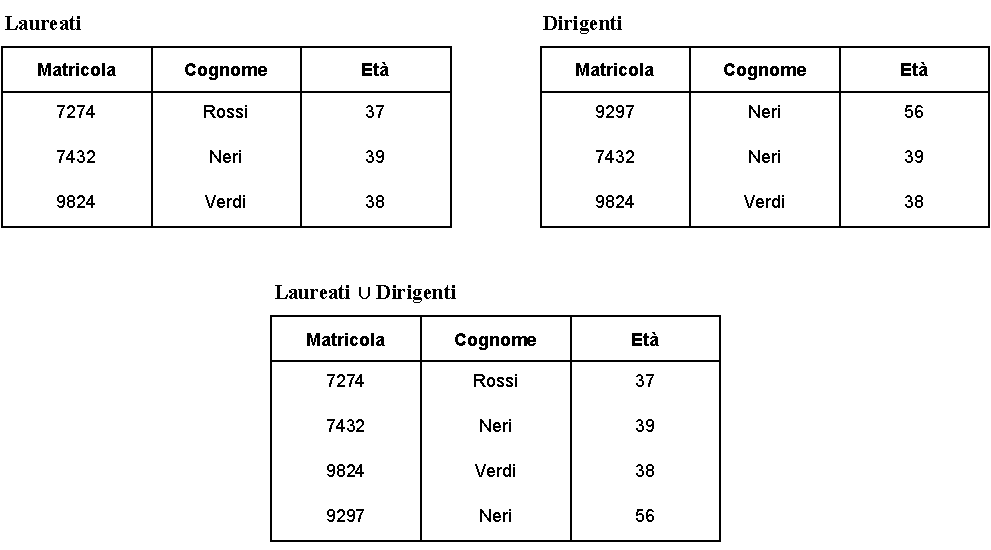
\includegraphics[width=\textwidth]{img/unione.pdf}
	\end{figure}

	\newpage
	
	\subsubsection{Intersezione}
	
	L'\textcolor{Red3}{\textbf{\underline{intersezione}}} di $r_{1}\left(X\right)$ e $r_{2}\left(X\right)$ è indicata con $r_{1} \cap r_{2}$ ed è una relazione su $X$ contenente le tuple che appartengono sia a $r_{1}$ sia a $r_{2}$.\newline
	
	\noindent
	La \textbf{cardinalità}, ovvero il numero di tuple contenute nella relazione del risultato:
	
	\begin{equation*}
		0 \le \left|r_{1} \cap r_{2}\right| \le \min\left(|r_{1}|, |r_{2}|\right)
	\end{equation*}
	
	\noindent
	\textcolor{Green4}{\textbf{\emph{Esempio}}}
	
	\begin{figure}[!htp]
		\centering
		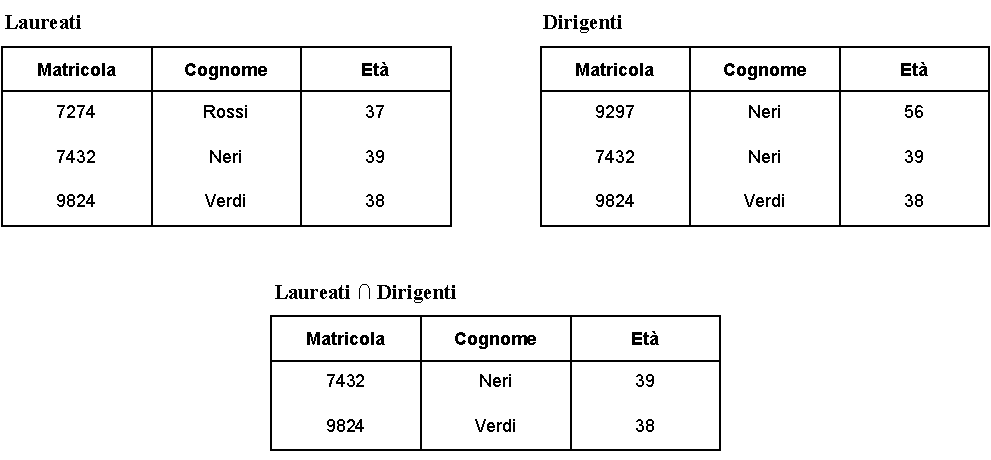
\includegraphics[width=\textwidth]{img/intersezione.pdf}
	\end{figure}

%	\newpage
	
	\subsubsection{Differenza}
	
	La \textcolor{Red3}{\textbf{\underline{differenza}}} di $r_{1}\left(X\right)$ e $r_{2}\left(X\right)$ è indicata con $r_{1} - r_{2}$ ed è una relazione su $X$ contenente le tuple che appartengono a $r_{1}$ e non appartengono a $r_{2}$.\newline
	
	\noindent
	La \textbf{cardinalità}, ovvero il numero di tuple contenute nella relazione del risultato:
	
	\begin{equation*}
		0 \le \left|r_{1} - r_{2}\right| \le |r_{1}|
	\end{equation*}

	\noindent
	\textcolor{Green4}{\textbf{\emph{Esempio}}}
	
	\begin{figure}[!htp]
		\centering
		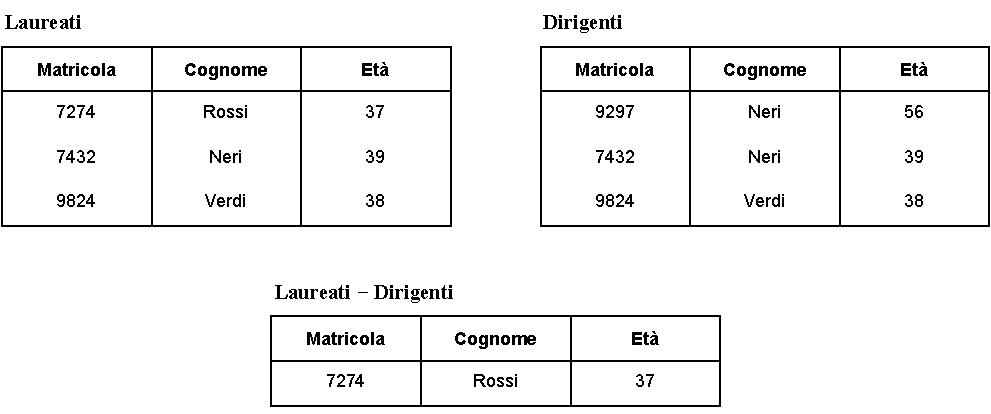
\includegraphics[width=\textwidth]{img/differenza.pdf}
	\end{figure}

	\newpage
	
	\subsection{Specifici}
	
	\subsubsection{Ridenominazione}
	
	L'\textcolor{Red3}{\textbf{\underline{obbiettivo}}} di questo operatore è risolvere le limitazioni degli operatori insiemistici. Infatti, esso \textbf{adegua i nomi degli attributi}, a seconda delle necessità, in particolare alla fine di facilitare le operazioni insiemistiche. Ovviamente, la ridenominazione avviene solamente sugli attributi, il \textbf{contenuto} rimane \textbf{inalterato}.\newline
	
	\noindent
	Il simbolo che lo rappresenta è la lettera greca rho $\rho$. \textbf{Al pedice viene inserita la ridenominazione, a destra il nome dell'attributo da rinominare e a sinistra il nuovo nome dell'attributo}. In generale, sia $r$ una relazione definita sull'insieme di attributi $X$ e sia $Y$ un (altro) insieme di attributi con la stessa cardinalità. Inoltre, siano $A_{1} A_{2} ... A_{k}$ e $B_{1} B_{2} ... B_{k}$ rispettivamente un ordinamento per gli attributi in $X$ e un ordinamento per quelli in $Y$. Allora la ridenominazione:
	
	\begin{equation*}
		\rho_{B_{1}B_{2} ... B_{k} \leftarrow A_{1}A_{2} ... A_{k}} \left(r\right)
	\end{equation*}

	\noindent
	Contiene una tupla $t'$ per ciascuna tupla $t$ in $r$, definita come segue: $t'$ è una tupla su $Y$ e $t\left[B_{i}\right] = t\left[A_{i}\right]$, per $i = 1, ..., k$.\newline
	
	\noindent
	La definizione conferma che ciò che cambia sono i nomi degli attributi, mentre i valori rimangono inalterati e vengono associati ai nuovi attributi.\newline
	
	\noindent
	\textcolor{Green4}{\textbf{\emph{Esempio}}}
	
	\begin{figure}[!htp]
		\centering
		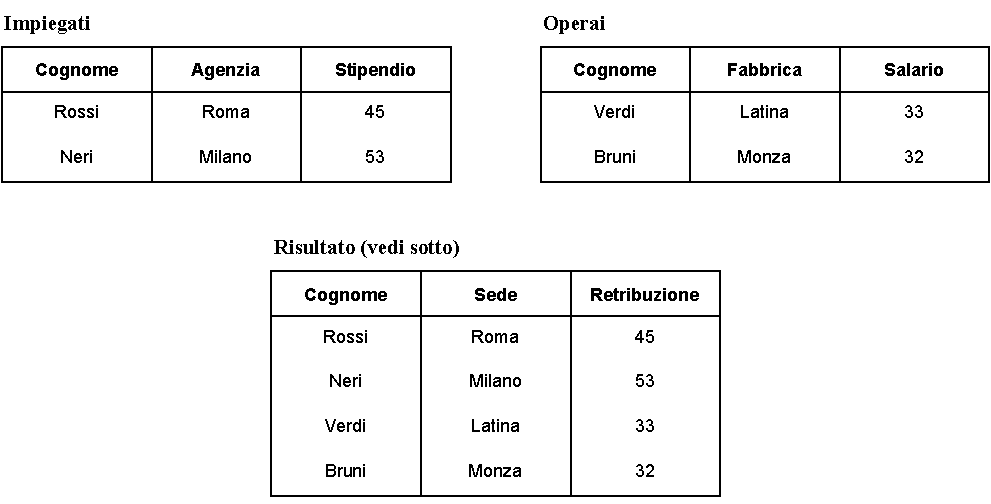
\includegraphics[width=\textwidth]{img/ridenominazione.pdf}
	\end{figure}

	\noindent
	Il risultato è ottenuto con la seguente operazione:
	
	\begin{equation*}
		\rho_{\text{ Sede, Retribuzione } \leftarrow \text{ Agenzia, Stipendio}} \left(\text{Impiegati}\right) \cup \rho_{\text{ Sede, Retribuzione } \leftarrow \text{ Fabbrica, Salario}}\left(\text{Operai}\right)
	\end{equation*}

	\newpage
	
	\subsubsection{Selezione}
	
	La selezione produce una porzione dell'operando. Più precisamente, la \textcolor{Red3}{\textbf{\underline{selezione}}} produce un sottoinsieme delle tuple su tutti gli attributi. Il \textbf{risultato contiene le tuple dell'operando che soddisfano la condizione di selezione}. Quest'ultima viene indicata nel pedice della notazione della selezione, ovvero sigma $\sigma$. Inoltre, le condizioni possono prevedere confronti fra attributi e confronti fra attributi e costanti, e possono essere complesse, ottenute combinando condizioni semplici con i connettivi logici $\lor$ (or), $\land$ (and) e $\lnot$ (not).\newline
	
	\noindent
	In generale, data una relazione $r\left(X\right)$, una \emph{forma proposizionale} $F$ su $X$ è una formula ottenuta combinando, con i connettivi $\land, \lor, \lnot$, condizioni atomiche del tipo $A\theta B$ o $A\theta c$, dove:
	
	\begin{itemize}
		\item $\theta$ è un \textbf{operatore di confronto}, il quale può essere:
		\begin{itemize}
			\item $=$
			\item $\ne$
			\item $>$
			\item $<$
			\item $\ge$
			\item $\le$
		\end{itemize}
	
		\item $A$ e $B$ sono \textbf{attributi} in $X$ sui cui valori il confronto $\theta$ abbia senso;
		
		\item $c$ è una \textbf{costante} \dquotes{compatibile} con il dominio di $A$ (cioè tale che il confronto $\theta$ sia definito).
	\end{itemize}
	
	\noindent
	Data una formula $F$ e una tupla $t$, è definito un valore di verità (cioè \dquotes{vero} o \dquotes{falso}) per $F$ su $t$:
	
	\begin{itemize}
		\item $A \theta B$ è vera su $t$ se $t\left[A\right]$ è in relazione $\theta$ con $t\left[B\right]$, altrimenti è falsa (per esempio, $A = B$ è vera su $t$ se e solo se $t\left[A\right] = t\left[B\right]$);
		
		\item $A \theta c$ è vera su $t$ se $t\left[A\right]$ è in relazione $\theta$ con $c$, altrimenti è falsa;
		
		\item $F_{1} \lor F_{2}, F_{1} \land F_{2}$ e $\lnot F_{1}$ hanno l'usuale significato.
	\end{itemize}

	\noindent
	La \textbf{\underline{definizione}}, in altre parole, è: la \textcolor{Red3}{\textbf{\underline{selezione}}} $\sigma_{F}\left(r\right)$, in cui $r$ è una relazione e $F$ una formula proposizionale, produce una relazione sugli stessi attributi di $r$ che contiene le tuple di $r$ su cui $F$ è vera.
	
	\newpage
	
	\noindent
	\textcolor{Green4}{\textbf{\emph{Esempio 1}}}
	
	\begin{figure}[!htp]
		\centering
		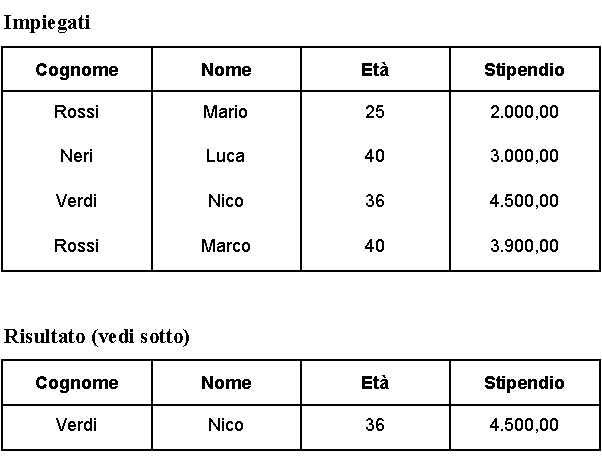
\includegraphics[width=0.8\textwidth]{img/selezione1.pdf}
	\end{figure}

	\noindent
	Il risultato è ottenuto con la seguente operazione:
	
	\begin{equation*}
		\sigma_{\text{Eta } > 30 \land \text{ Stipendio } > 4.000,00}\left(\text{Impiegati}\right)
	\end{equation*}

	\noindent
	\textcolor{Green4}{\textbf{\emph{Esempio 2}}}
	
	\begin{figure}[!htp]
		\centering
		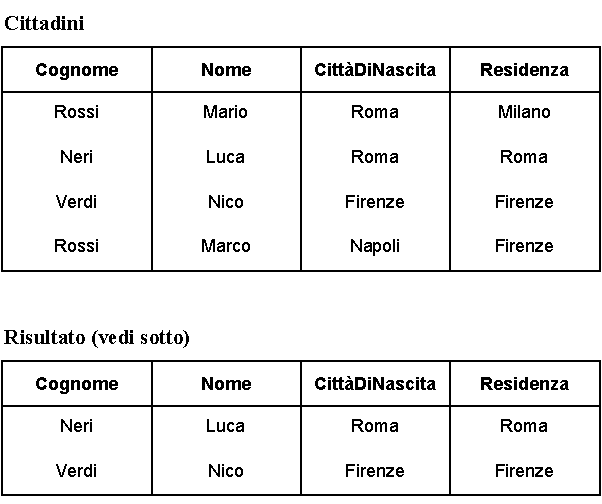
\includegraphics[width=0.8\textwidth]{img/selezione2.pdf}
	\end{figure}

	\noindent
	Il risultato è ottenuto con la seguente operazione:
	
	\begin{equation*}
		\sigma_{\text{CittàDiNascita } = \text{ Residenza}}\left(\text{Cittadini}\right)
	\end{equation*}
	
	\newpage
	
	\subsubsection{Proiezione}
	
	La \textcolor{Red3}{\textbf{\underline{proiezione}}} dà un risultato cui contribuiscono tutte le tuple, ma su un sottoinsieme degli attributi.
	
	Formalmente, dati una relazione $r\left(X\right)$ e un sottoinsieme $Y$ di $X$, la \textbf{proiezione} di $r$ su $Y$ (indicata con $\pi_{Y}\left(r\right)$) è l'insieme di tuple su $Y$ ottenute dalle tuple di $r$ considerando solo i valori su $Y$:
	
	\begin{equation*}
		\pi_{Y}\left(r\right) = \left\{t\left[Y\right] \: | \: t \in r\right\}
	\end{equation*}

	\noindent
	Dagli esempi è chiaro che la proiezione permette di decomporre verticalmente le relazioni.\newline
	
	\noindent
	\textcolor{Green4}{\textbf{\emph{Esempio 1}}}\newline
	
	\noindent
	In questo caso, il risultato della proiezione contiene tante tuple quante l'operando, definite però solo su parte degli attributi.
	
	\begin{figure}[!htp]
		\centering
		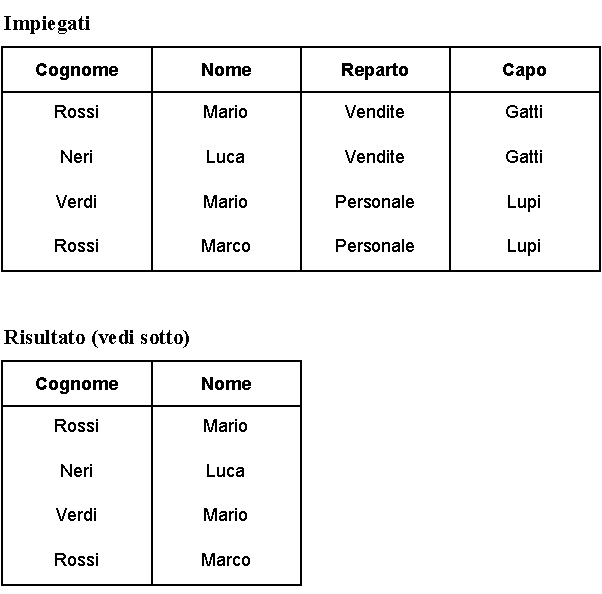
\includegraphics[width=0.9\textwidth]{img/proiezione1.pdf}
	\end{figure}
	
	\noindent
	Il risultato è ottenuto con la seguente operazione:
	
	\begin{equation*}
		\pi_{\text{Cognome, Nome }}\left(\text{Impiegati}\right)
	\end{equation*}

	\newpage
	
	\noindent
	\textcolor{Green4}{\textbf{\emph{Esempio 2}}}\newline
	
	\noindent
	In questo caso, il risultato contiene un numero di tuple inferiore rispetto a quelle dell'operando, perché alcune tuple, avendo uguali valori su tutti gli attributi della proiezione, danno lo stesso contributo alla proiezione stessa. Essendo le relazioni definite come insieme, non possono, per definizione, in esse comparire più tuple uguale fra loro: i contributi \dquotes{collassano} in una sola tupla.
	
	\begin{figure}[!htp]
		\centering
		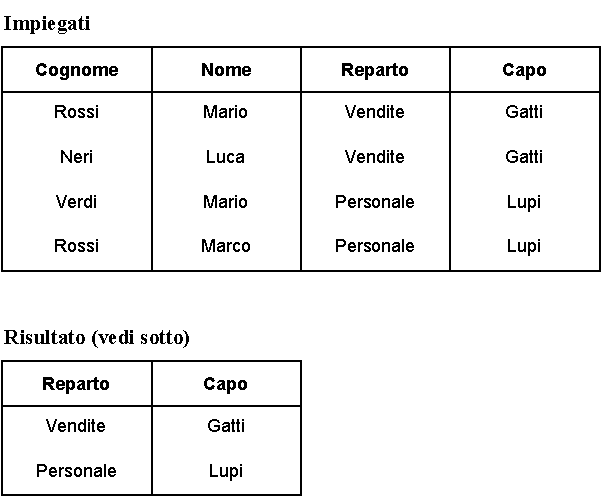
\includegraphics[width=0.9\textwidth]{img/proiezione2.pdf}
	\end{figure}
	
	\noindent
	Il risultato è ottenuto con la seguente operazione:
	
	\begin{equation*}
		\pi_{\text{Reparto, Capo }}\left(\text{Impiegati}\right)
	\end{equation*}
	
	\newpage
	
	\subsection{Join}
	
	L'operatore di \emph{join} consente di correlare dati contenuti in relazioni diverse, confrontando i valori contenuti in esse e utilizzando quindi la caratteristica fondamentale del modello, ovvero quella di essere basta su valori.
	
	Formalmente, due relazione $r_{1}$ e $r_{2}$ di schema $X_{1}$ e $X_{2}$ rispettivamente, gli operatori di \emph{join} generano tuple $t$ nella relazione risultato a partire dalle coppie di tuple $\left(t_{1}, t_{2}\right) \in r_{1} \times r_{2}$ che soddisfano una certa condizione (chiamata \textbf{predicato di join}).
	
	\subsubsection{Join naturale}
	
	Il \textcolor{Red3}{\textbf{\underline{join naturale}}} è un operatore che correla dati in relazioni diverse, sulla base di valori uguali in attributi con lo stesso nome (si veda l'esempio come chiarificatore). Questa operazione viene denotata con il simbolo $\Join$.
	
	Il \textbf{risultato} dell'operatore è una relazione sull'unione degli insiemi di attributi degli operandi e le sue tuple sono ottenute combinando le tuple degli operandi con valori uguali sugli attributi comuni. Nel primo esempio sotto, la prima tupla del \emph{join} deriva dalla combinazione della prima tupla della relazione $r_{1}$ e dalla seconda tupla della relazione $r_{2}$.\newline
	
	\noindent
	Formalmente, il \textbf{join naturale} $r_{1} \Join r_{2}$ di $r_{1}\left(X_{1}\right)$ e $r_{2}\left(X_{2}\right)$ è una relazione definita su $X_{1}X_{2}$ (cioè sull'unione degli insiemi $X_{1}$ e $X_{2}$), come segue:
	
	\begin{equation*}
		r_{1} \Join r_{2} = \left\{t \text{ su } X_{1}X_{2} \:\: | \:\: t\left[X_{1}\right] \in r_{1}, t\left[X_{2}\right] \in r_{2}\right\}
	\end{equation*}

	\noindent
	Si noti che è molto frequente eseguire \emph{join} sulla base di valori della chiave di una delle relazioni coinvolte, esplicitando i riferimenti fra tuple che sono realizzati per mezzo di valori soprattutto valori di chiavi. Osservando l'esempio 2, si vede che ciascuna delle tuple di \textsf{Infrazioni} è stata combinata con una e una sola delle tuple di \textsf{Auto}:
	
	\begin{itemize}
		\item  Una sola perché \textsf{Prov} e \textsf{Numero} formano una chiave di \textsf{Auto};
		\item Almeno una perché è definito il vincolo di integrità referenziale fra \textsf{Prov} e \textsf{Numero} in \textsf{Infrazioni} e (la chiave primaria di) \textsf{Auto}
	\end{itemize}

	\noindent
	Dunque, il \emph{join} ha esattamente tante tuple quante la relazione \textsf{Infrazioni}.
	
	\newpage
	
	\noindent
	\textcolor{Green4}{\textbf{\emph{Esempio 1}}}
	
	\begin{figure}[!htp]
		\centering
		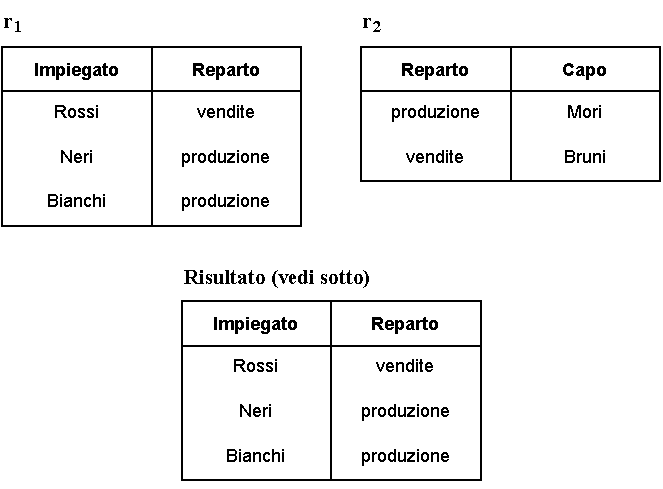
\includegraphics[width=0.65\textwidth]{img/join_naturale1.pdf}
	\end{figure}
	
	\noindent
	Il risultato è ottenuto con la seguente operazione:
	
	\begin{equation*}
		r_{1} \Join r_{2}
	\end{equation*}

	\noindent
	\textcolor{Green4}{\textbf{\emph{Esempio 2}}}
	
	\begin{figure}[!htp]
		\centering
		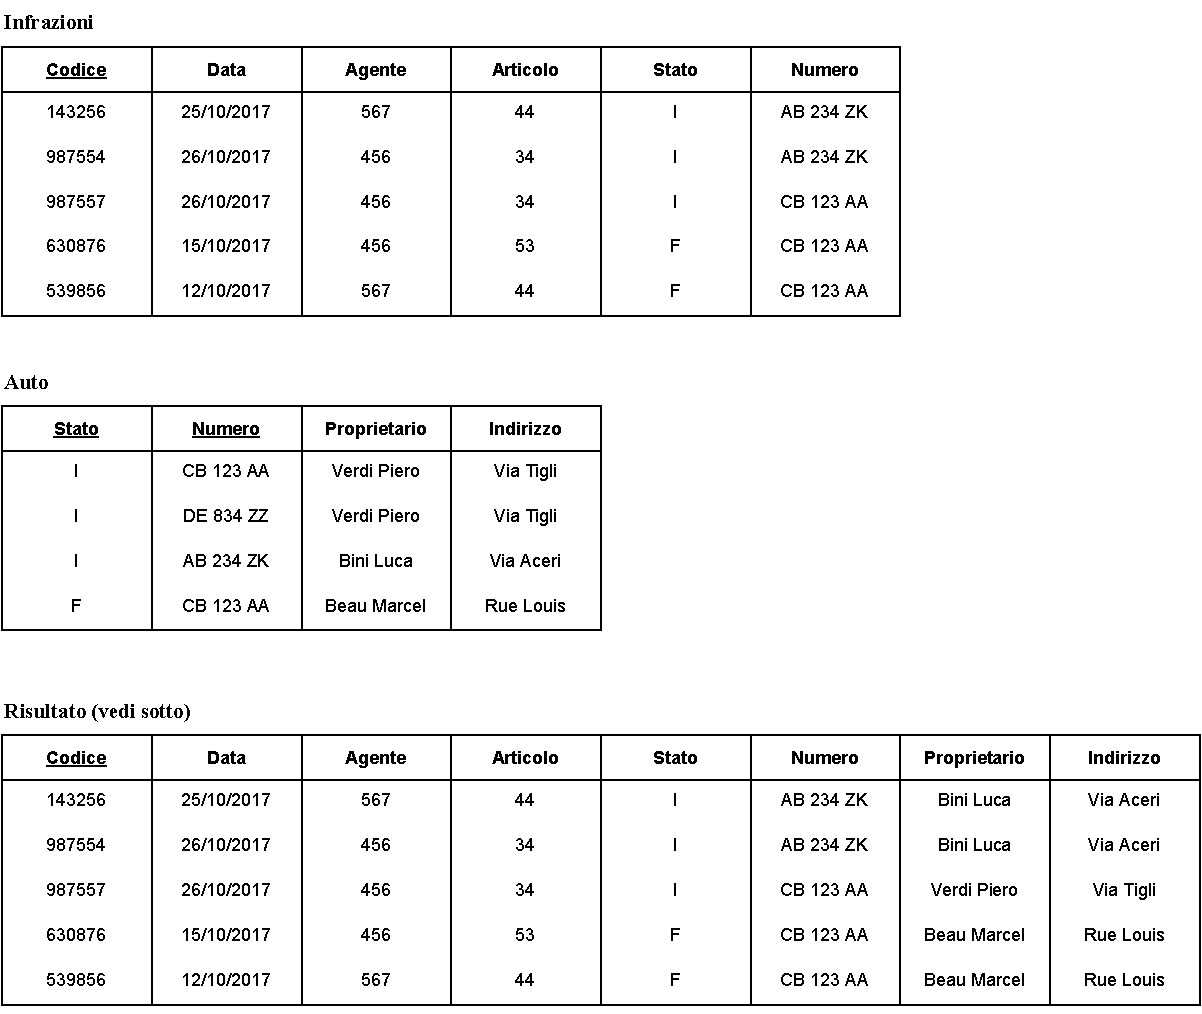
\includegraphics[width=\textwidth]{img/join_naturale2.pdf}
	\end{figure}
	
	\noindent
	Il risultato è ottenuto con la seguente operazione:
	
	\begin{equation*}
		\textsf{Infrazioni} \Join \textsf{Auto}
	\end{equation*}

	\newpage
	
	\subsubsection{Join completi e incompleti}
	
	Nell'esempio 1 nel paragrafo del \emph{join naturale}, si può dire che ciascuna tupla di ciascuno degli operandi contribuisce almeno una tupla del risultato (in questo caso il \emph{join} viene detto \textcolor{Red3}{\textbf{\underline{completo}}}): per ogni tupla $t_{1}$ di $r_{1}$, esiste una tupla $t$ in $r_{1} \Join r_{2}$ tale che $t\left[X_{1}\right] = t_{1}$ (e analogamente per $r_{2}$).
	
	L'esempio 1 a fine paragrafo, mostra un \emph{join} in cui alcune tuple degli operandi, in particolare la prima di $r_{1}$ e la seconda di $r_{2}$, non contribuiscono al risultato, perché l'altra relazione non contiene tuple con gli stessi valori sull'attributo comune. In questo caso il \emph{join} viene detto \textcolor{Red3}{\textbf{\underline{dangling}}}, ovvero \textbf{\emph{dondolante}}.
	
	Infine, come caso limite, è ovviamente possibile che nessuna delle tuple degli operandi sia combinabile, e allora il risultato del \emph{join} è la \textcolor{Red3}{\textbf{\underline{relazione vuota}}} (esempio 2 a fine paragrafo). All'estremo opposto, è possibile che ciascuna delle tuple di ciascuno degli operandi sia combinabile con tutte dell'altro, come mostrato nell'ultimo esempio del paragrafo, e in questo caso il risultato ha un numero di tuple pari al prodotto delle cardinalità degli operandi e cioè $|r_{1}| \times |r_{2}|$ (dove $|r|$ indica la cardinalità della relazione $r$).\newline
	
	\noindent
	Alcune osservazioni finali:
	\begin{itemize}
		\item Se il \emph{join} di $r_{1}$ e $r_{2}$ è completo, allora contiene almeno un numero di tuple pari al massimo fra $|r_{1}|$ e $|r_{2}|$;
		
		\item Se $X_{1} \cap X_{2}$ contiene una chiave per $r_{2}$, allora il \emph{join} di $r_{1}\left(X_{1}\right)$ e $r_{2}\left(X_{2}\right)$ contiene al più $|r_{1}|$ tuple;
		
		\item Se $X_{1} \cap X_{2}$ coincide con una chiave per $r_{2}$ e sussiste il vincolo di riferimento fra $X_{1} \cap X_{2}$ in $r_{1}$ e la chiave di $r_{2}$, allora il \emph{join} di $r_{1}\left(X_{1}\right)$ e $r_{2}\left(X_{2}\right)$ contiene esattamente $|r_{1}|$ tuple.
	\end{itemize}

	\newpage

	\noindent
	\textcolor{Green4}{\textbf{\emph{Esempio 1}}}
	
	\begin{figure}[!htp]
		\centering
		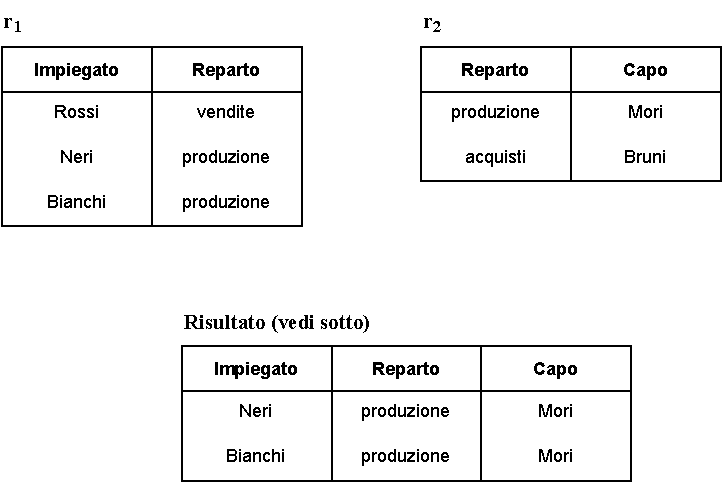
\includegraphics[width=0.9\textwidth]{img/join_dangling.pdf}
	\end{figure}
	
	\noindent
	Il risultato è ottenuto con la seguente operazione:
	\begin{equation*}
		r_{1} \Join r_{2}
	\end{equation*}
	
	\noindent
	\textcolor{Green4}{\textbf{\emph{Esempio 2}}}
	
	\begin{figure}[!htp]
		\centering
		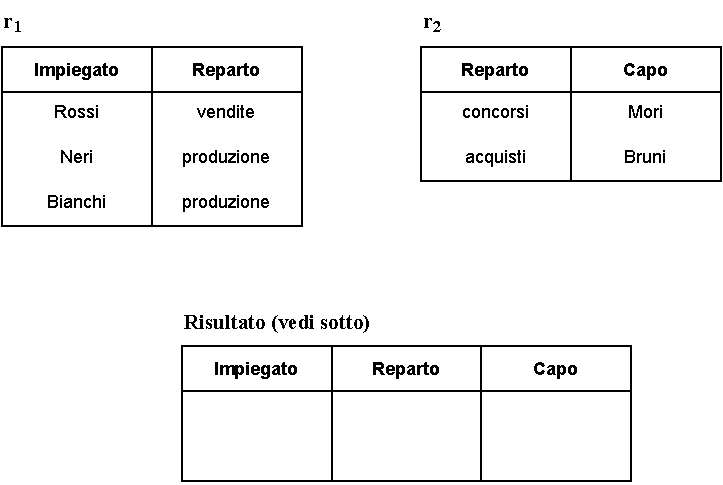
\includegraphics[width=0.9\textwidth]{img/join_vuoto.pdf}
	\end{figure}
	
	\noindent
	Il risultato è ottenuto con la seguente operazione:
	\begin{equation*}
		r_{1} \Join r_{2}
	\end{equation*}

	\newpage

	\noindent
	\textcolor{Green4}{\textbf{\emph{Esempio 3}}}

	\begin{figure}[!htp]
		\centering
		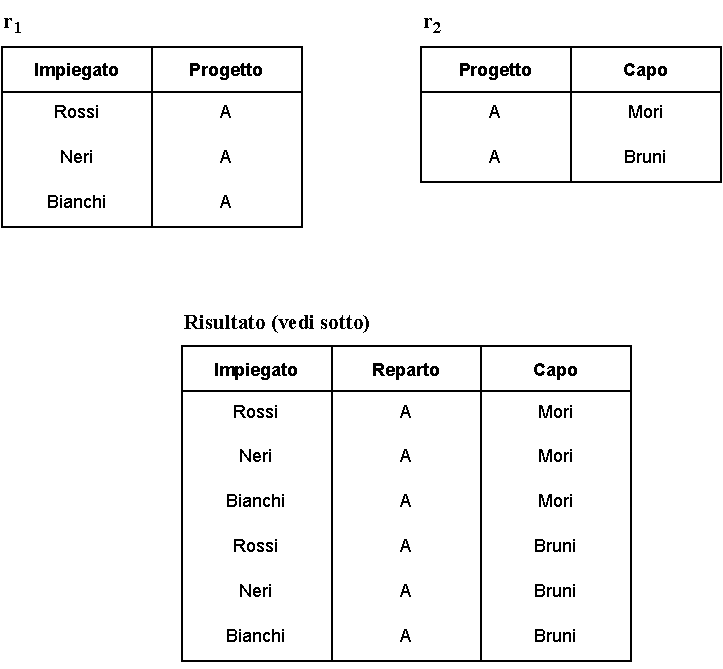
\includegraphics[width=0.9\textwidth]{img/join_massimo.pdf}
	\end{figure}
	
	\noindent
	Il risultato è ottenuto con la seguente operazione:
	\begin{equation*}
		r_{1} \Join r_{2}
	\end{equation*}\newpage

	\subsubsection{Theta-join ed equi-join}
	
	Osservando l'esempio 1 a fine paragrafo, è possibile notare come un prodotto cartesiano ha di solito ben poca utilità, in quanto concatena tuple non necessariamente correlate dal punto di vista semantico. Infatti, il \textbf{prodotto cartesiano viene spesso seguito da una selezione}, la quale centra l'attenzione su tuple correlate secondo le esigenze. \textcolor{Green4}{\textbf{Per esempio}}, nell'esempio 2 a fine paragrafo, sulle relazione \textsf{Impiegati} e \textsf{Progetti} ha senso definire un prodotto cartesiano seguito dalla selezione che mantiene solo le tuple con valori uguali sull'attributo \textsf{\emph{Progetto}} di \textsf{Impiegati} e su \textsf{\emph{Codice}} di \textsf{Progetti}.
	
	Per questo motivo, viene definito un operatore derivato (cioè per mezzo di altri operatori), chiamato \textcolor{Red3}{\textbf{\underline{theta-join}}}. Esso è considerato come un \textbf{prodotto cartesiano seguito da una selezione}, nel modo seguente:
	\begin{equation*}
		r_{1} \underset{F}{\Join} r_{2} = \sigma_{F}\left(r_{1} \Join r_{2}\right)
	\end{equation*}
	
	\subsection{Algebra con valori nulli}
	
	\subsection{Equivalenza di espressioni algebriche}
	
	
\end{document}